\chapter{Annexe : Complément d'analyse } \label{chap:appC}
% PRL Mtt

\begin{fmffile}{appendixC}

\section{Datasets pour les données 2016 et 2017}

\subsection{Liste des déclencheurs}\label{HLTpath}

\begin{table}[H]
\resizebox{\textwidth}{!}{
\begin{tabular}{ccc}
    \noalign{\smallskip}\hline\noalign{\smallskip}
    Année & Chemin de déclenchement & Jeu de données \\
    \noalign{\smallskip}
    \hline \hline
    \noalign{\smallskip}
      2016 & HLT\_Mu23\_TrkIsoVVL\_Ele12\_CaloIdL\_TrackIdL\_IsoVL\_v*&  Donnée Run B-G \& MC\\
      2016 &HLT\_Mu8\_TrkIsoVVL\_Ele23\_CaloIdL\_TrackIdL\_IsoVL\_v* & Donnée Run B-G \& MC\\
      2016 & HLT\_Mu23\_TrkIsoVVL\_Ele12\_CaloIdL\_TrackIdL\_IsoVL\_DZ\_v* & Donnée Run H \\ 
      2016 & HLT\_Mu8\_TrkIsoVVL\_Ele23\_CaloIdL\_TrackIdL\_IsoVL\_DZ\_v*  & Donnée Run H\\ 
      2016 & HLT\_IsoMu24\_v*  & Donnée \& MC \\
      2016 & HLT\_IsoTkMu24\_v*  & Donnée \& MC \\
      2016 & HLT\_Ele27\_WPTight\_Gsf\_v*  & Donnée \& MC \\
    \noalign{\smallskip}\hline\noalign{\smallskip}
      2017 & Mu8\_TrkIsoVVL\_Ele23\_CaloIdL\_TrackIdL\_IsoVL\_DZ\_v* & Donnée \& MC \\ 
      2017 &   Mu23\_TrkIsoVVL\_Ele12\_CaloIdL\_TrackIdL\_IsoVL\_v*  & Donnée \& MC \\
      2017 & IsoMu27\_v*  & Donnée \& MC \\
      2017 & Ele35\_WPTight\_Gsf\_v*  & Donnée \& MC \\
    \noalign{\smallskip}\hline\noalign{\smallskip}
\end{tabular}
}
\caption{Chemin de déclenchement utilisé à \SI{13}{\TeV} pour les prises de données de l'année 2016 et 2017.}
\end{table}

\subsection{Liste des échantillons Monte-Carlo}\label{MC2016}

\begin{table}
\resizebox{\textwidth}{!}{
\begin{tabular}{ccc}
    \noalign{\smallskip}\hline\noalign{\smallskip}
    Échantillons MC 2016 & Évènements & Section efficace $\times$ BR (pb) \\
    \noalign{\smallskip}
    \hline \hline
    \noalign{\smallskip}
  /TTTo2L2Nu\_TuneCP5\_PSweights\_13TeV-powheg-pythia8/
  & 67 860 400 & 89.05 (NNLO) \\
  /TTToSemiLeptonic\_TuneCP5\_PSweights\_13TeV-powheg-pythia8/
  & 107 604 800 & 366.9 (NNLO)  \\
  /TTToHadronic\_TuneCP5\_PSweights\_13TeV-powheg-pythia8/
  & 68 518 800 & 377.96 \\
    \noalign{\smallskip}\hline\noalign{\smallskip}
  /ST\_s-channel\_4f\_leptonDecays\_TuneCP5\_PSweights\_13TeV-amcatnlo-pythia8/
  & 9 842 599 & 10.32 (NLO) \\
  /ST\_t-channel\_top\_4f\_inclusiveDecays\_TuneCP5\_13TeV-powhegV2-madspin-pythia8/
  & 31 848 000 & 136.02 (NLO)  \\
  /ST\_t-channel\_antitop\_4f\_inclusiveDecays\_TuneCP5\_13TeV-powhegV2-madspin-pythia8/
  & 17 780 700 & 80.95 (NLO)  \\
  /ST\_tW\_top\_5f\_inclusiveDecays\_TuneCP5\_PSweights\_13TeV-powheg-pythia8/
  & 4 983 500 & 35.85  (NLO) \\
  /ST\_tW\_antitop\_5f\_inclusiveDecays\_TuneCP5\_PSweights\_13TeV-powheg-pythia8/
  & 4 980 600 & 35.85 (NLO)  \\
  /TTWJetsToLNu\_TuneCUETP8M1\_13TeV-amcatnloFXFX-madspin-pythia8
  & 5 280 565 %2160168+3120397
  & 0.2043 (NLO)  \\
  /TTWJetsToQQ\_TuneCUETP8M1\_13TeV-amcatnloFXFX-madspin-pythia8/
  & 833 298 & 0.4062 \\
  /TTZToLLNuNu\_M-10\_TuneCUETP8M1\_13TeV-amcatnlo-pythia8/
  & 13 764 447 %1992438+5837781+5934228
  & 0.2529 (NLO)  \\
  /TTZToQQ\_TuneCUETP8M1\_13TeV-amcatnlo-pythia8/ & 749 400 & 0.5297 \\
  /WW\_TuneCUETP8M1\_13TeV-pythia8/ & 7 982 180 %994012+6988168
  & 118.7(NNLO) \\
  /WZ\_TuneCUETP8M1\_13TeV-pythia8/ & 3 997 571 %1000000+2997571
  & 47.13 \\
  /ZZ\_TuneCUETP8M1\_13TeV-pythia8/ & 1 988 098 %990064+998034
  & 16.523 \\
  /WJetsToLNu\_TuneCUETP8M1\_13TeV-madgraphMLM-pythia8/ & 261 383 472 %24120319+237263153
  & 61526.7 \\
  /DYJetsToLL\_M-10to50\_TuneCUETP8M1\_13TeV-madgraphMLM-pythia8/ & 139 138 448 & 22635.1 \\ %67981236+30792978+40364234
  /DYJetsToLL\_M-50\_TuneCUETP8M1\_13TeV-amcatnloFXFX-pythia8/ & 120 777 245 & 6225.4 \\
    \noalign{\smallskip}\hline\noalign{\smallskip}
\end{tabular}
}
\caption{Liste des échantillons Monte-Carlo pour l'année 2016 ainsi que leur nombre d'évènements et leur section efficace pondérée par leur rapport d'embranchement (BR).}
\end{table}

\begin{table}
\resizebox{\textwidth}{!}{
\begin{tabular}{ccc}
    \noalign{\smallskip}\hline\noalign{\smallskip}
    Échantillons MC 2017 & Évènements & Section efficace $\times$ BR (pb) \\
    \noalign{\smallskip}
    \hline \hline
    \noalign{\smallskip}
  /TTTo2L2Nu\_TuneCP5\_PSweights\_13TeV-powheg-pythia8/
  & 69 155 808 & 89.05 (NNLO) \\
  /TTToSemiLeptonic\_TuneCP5\_PSweights\_13TeV-powheg-pythia8/
  & 110 014 744 & 365.3 (NNLO) \\
  /TTToHadronic\_TuneCP5\_PSweights\_13TeV-powheg-pythia8/
  & 130 262 440 & 380.11 \\
    \noalign{\smallskip}\hline\noalign{\smallskip}
  /ST\_s-channel\_4f\_leptonDecays\_TuneCP5\_13TeV-amcatnlo-pythia8/
  & 19 798 753 & 10.32 (NLO) \\ %9883805 + 9914948
  %/ST\_s-channel\_4f\_leptonDecays\_TuneCP5\_PSweights\_13TeV-amcatnlo-pythia8/
  %& 9 914 948 & 10.32 (NLO) \\
  /ST\_t-channel\_top\_4f\_inclusiveDecays\_TuneCP5\_13TeV-powhegV2-madspin-pythia8/
  & 5 982 064 & 136.02 (NLO) \\
  /ST\_t-channel\_antitop\_4f\_inclusiveDecays\_TuneCP5\_13TeV-powhegV2-madspin-pythia8/
  & 3 675 910 & 80.95 (NLO) \\
  /ST\_tW\_top\_5f\_inclusiveDecays\_TuneCP5\_13TeV-powheg-pythia8/
  & 15 739 428 & 35.5 (NNLO)\\ % 7794186 + 7945242
  %/ST\_tW\_top\_5f\_inclusiveDecays\_TuneCP5\_PSweights\_13TeV-powheg-pythia8/
  %& 7 945 242 & 35.5 (NNLO) \\
  /ST\_tW\_antitop\_5f\_inclusiveDecays\_TuneCP5\_13TeV-powheg-pythia8/
  & 15 722 706 & 35.5 (NNLO) \\ % 7977430  + 7745276
  %/ST\_tW\_antitop\_5f\_inclusiveDecays\_TuneCP5\_PSweights\_13TeV-powheg-pythia8/
  %& 7 745 276 & 35.5 (NNLO) \\
  /TTWJetsToLNu\_TuneCP5\_13TeV-amcatnloFXFX-madspin-pythia8/
  & 9 903 448 & 0.2043 (NLO) \\
  /TTWJetsToQQ\_TuneCP5\_13TeV-amcatnloFXFX-madspin-pythia8/
  & 811 306 & 0.4062 \\
  /TTZToLLNuNu\_M-10\_TuneCP5\_13TeV-amcatnlo-pythia8/
  &  19 024 650 & 0.2529 (NLO) \\
  /TTZToQQ\_TuneCP5\_13TeV-amcatnlo-pythia8/
  & 750 000 & 0.5297 \\
  /WW\_TuneCP5\_13TeV-pythia8/ & 7 765 828  & 118.7 (NNLO) \\
  /WZ\_TuneCP5\_13TeV-pythia8/ & 3 928 630 & 47.13 \\
  /ZZ\_TuneCP5\_13TeV-pythia8/ & 1 925 931 & 16.523 \\
  /WJetsToLNu\_TuneCP5\_13TeV-madgraphMLM-pythia8/ & 77 700 506 & 0.4062 \\
  %/WJetsToLNu\_TuneCP5\_13TeV-madgraphMLM-pythia8/ & 30 008 250 & 61526.7 \\
  /DYJetsToLL\_M-10to50\_TuneCP5\_13TeV-madgraphMLM-pythia8/ & 39 536 839 & 22635.1\\
  /DYJetsToLL\_M-50\_TuneCP5\_13TeV-amcatnloFXFX-pythia8/ &  209 630 730 & 6225.4 \\
    \noalign{\smallskip}\hline\noalign{\smallskip}
\end{tabular}
}
\caption{Liste des échantillons Monte-Carlo pour l'année 2017 ainsi que leur nombre d'évènements et leur section efficace pondérée par leur facteur d'embranchement (BR).}
\end{table}

\subsection{Liste des échantillons de données}

\begin{table}[H]
\begin{subtable}[b]{0.45\textwidth}
\resizebox{\textwidth}{!}{
\begin{tabular}{cc}
    \noalign{\smallskip}\hline\noalign{\smallskip}
    Données 2016 & Luminosité intégrée \\
    \noalign{\smallskip}
    \hline \hline
    \noalign{\smallskip}
  /MuonEG/Run2016B-17Jul2018\_ver2-v1/ &  5.75 fb$^{-1}$\\
  /MuonEG/Run2016C-17Jul2018-v1/ &  2.57 fb$^{-1}$\\
  /MuonEG/Run2016D-17Jul2018-v1/ &  4.24 fb$^{-1}$\\
  /MuonEG/Run2016E-17Jul2018-v2/ &  4.02 fb$^{-1}$\\
  /MuonEG/Run2016F-17Jul2018-v1/ &  3.1 fb$^{-1}$ \\
  /MuonEG/Run2016G-17Jul2018-v1/ &  7.57 fb$^{-1}$ \\
  /MuonEG/Run2016G-17Jul2018-v1/ &  8.65 fb$^{-1}$ \\
    \noalign{\smallskip}\hline\noalign{\smallskip}
  /SingleMuon/Run2016B-17Jul2018\_ver2-v1/ & 5.75 fb$^{-1}$ \\
  /SingleMuon/Run2016C-17Jul2018-v1/ & 2.57 fb$^{-1}$ \\
  /SingleMuon/Run2016D-17Jul2018-v1/ & 4.24 fb$^{-1}$ \\
  /SingleMuon/Run2016E-17Jul2018-v2/ & 4.02 fb$^{-1}$ \\
  /SingleMuon/Run2016F-17Jul2018-v1/ & 3.1 fb$^{-1}$ \\
  /SingleMuon/Run2016G-17Jul2018-v1/ & 7.57 fb$^{-1}$ \\
  /SingleMuon/Run2016H-17Jul2018-v1/ & 8.65 fb$^{-1}$ \\
    \noalign{\smallskip}\hline\noalign{\smallskip}
  /SingleElectron/Run2016B-17Jul2018\_ver2-v1/ & 5.75 fb$^{-1}$ \\
  /SingleElectron/Run2016C-17Jul2018-v1/ & 2.57 fb$^{-1}$ \\
  /SingleElectron/Run2016D-17Jul2018-v1/ & 4.24 fb$^{-1}$ \\
  /SingleElectron/Run2016E-17Jul2018-v2/ & 4.02 fb$^{-1}$ \\
  /SingleElectron/Run2016F-17Jul2018-v1/ & 3.1 fb$^{-1}$ \\
  /SingleElectron/Run2016G-17Jul2018-v1/ & 7.57 fb$^{-1}$ \\
  /SingleElectron/Run2016H-17Jul2018-v1/ & 8.65 fb$^{-1}$ \\
    \noalign{\smallskip}\hline\noalign{\smallskip}
\end{tabular}
}
\end{subtable}
\hfill
\begin{subtable}[b]{0.45\textwidth}
\resizebox{\textwidth}{!}{
\begin{tabular}{cc}
    \noalign{\smallskip}\hline\noalign{\smallskip}
    Données 2017 & Luminosité intégrée \\
    \noalign{\smallskip}
    \hline \hline
    \noalign{\smallskip}
  /MuonEG/Run2017B-31Mar2018-v1/ & 4.77 fb$^{-1}$\\
  /MuonEG/Run2017C-31Mar2018-v1/ & 9.58 fb$^{-1}$\\
  /MuonEG/Run2017D-31Mar2018-v1/ & 4.22 fb$^{-1}$\\
  /MuonEG/Run2017E-31Mar2018-v1/ & 9.26 fb$^{-1}$\\
  /MuonEG/Run2017F-31Mar2018-v1/ & 13.46 fb$^{-1}$ \\
    \noalign{\smallskip}\hline\noalign{\smallskip}
  /SingleMuon/Run2017B-31Mar2018-v1/ & 4.77 fb$^{-1}$ \\
  /SingleMuon/Run2017C-31Mar2018-v1/ & 9.58 fb$^{-1}$ \\
  /SingleMuon/Run2017D31Mar2018-v1/ & 4.22 fb$^{-1}$ \\
  /SingleMuon/Run2017E-31Mar2018-v1/ & 9.26 fb$^{-1}$ \\
  /SingleMuon/Run2017F-31Mar2018-v1/ & 13.46 fb$^{-1}$ \\
    \noalign{\smallskip}\hline\noalign{\smallskip}
  /SingleElectron/Run2017B-31Mar2018-v1/ & 4.77 fb$^{-1}$ \\
  /SingleElectron/Run2017C-31Mar2018-v1/ & 9.58 fb$^{-1}$ \\
  /SingleElectron/Run2017D-31Mar2018-v1/ & 4.22 fb$^{-1}$ \\
  /SingleElectron/Run2017E-31Mar2018-v1/ & 9.26 fb$^{-1}$ \\
  /SingleElectron/Run2017F-31Mar2018-v1/ & 13.46 fb$^{-1}$ \\
    \noalign{\smallskip}\hline\noalign{\smallskip}
\end{tabular}
}
\end{subtable}
\caption{Echantillons de données 2016 et 2017}
\end{table}



\section{Facteurs correctifs sur les Monte-Carlo}

\subsection{Reconstruction, isolation, identification, des électrons et des muons}\label{app:sfem}

\begin{figure}[H]
    \begin{center}
        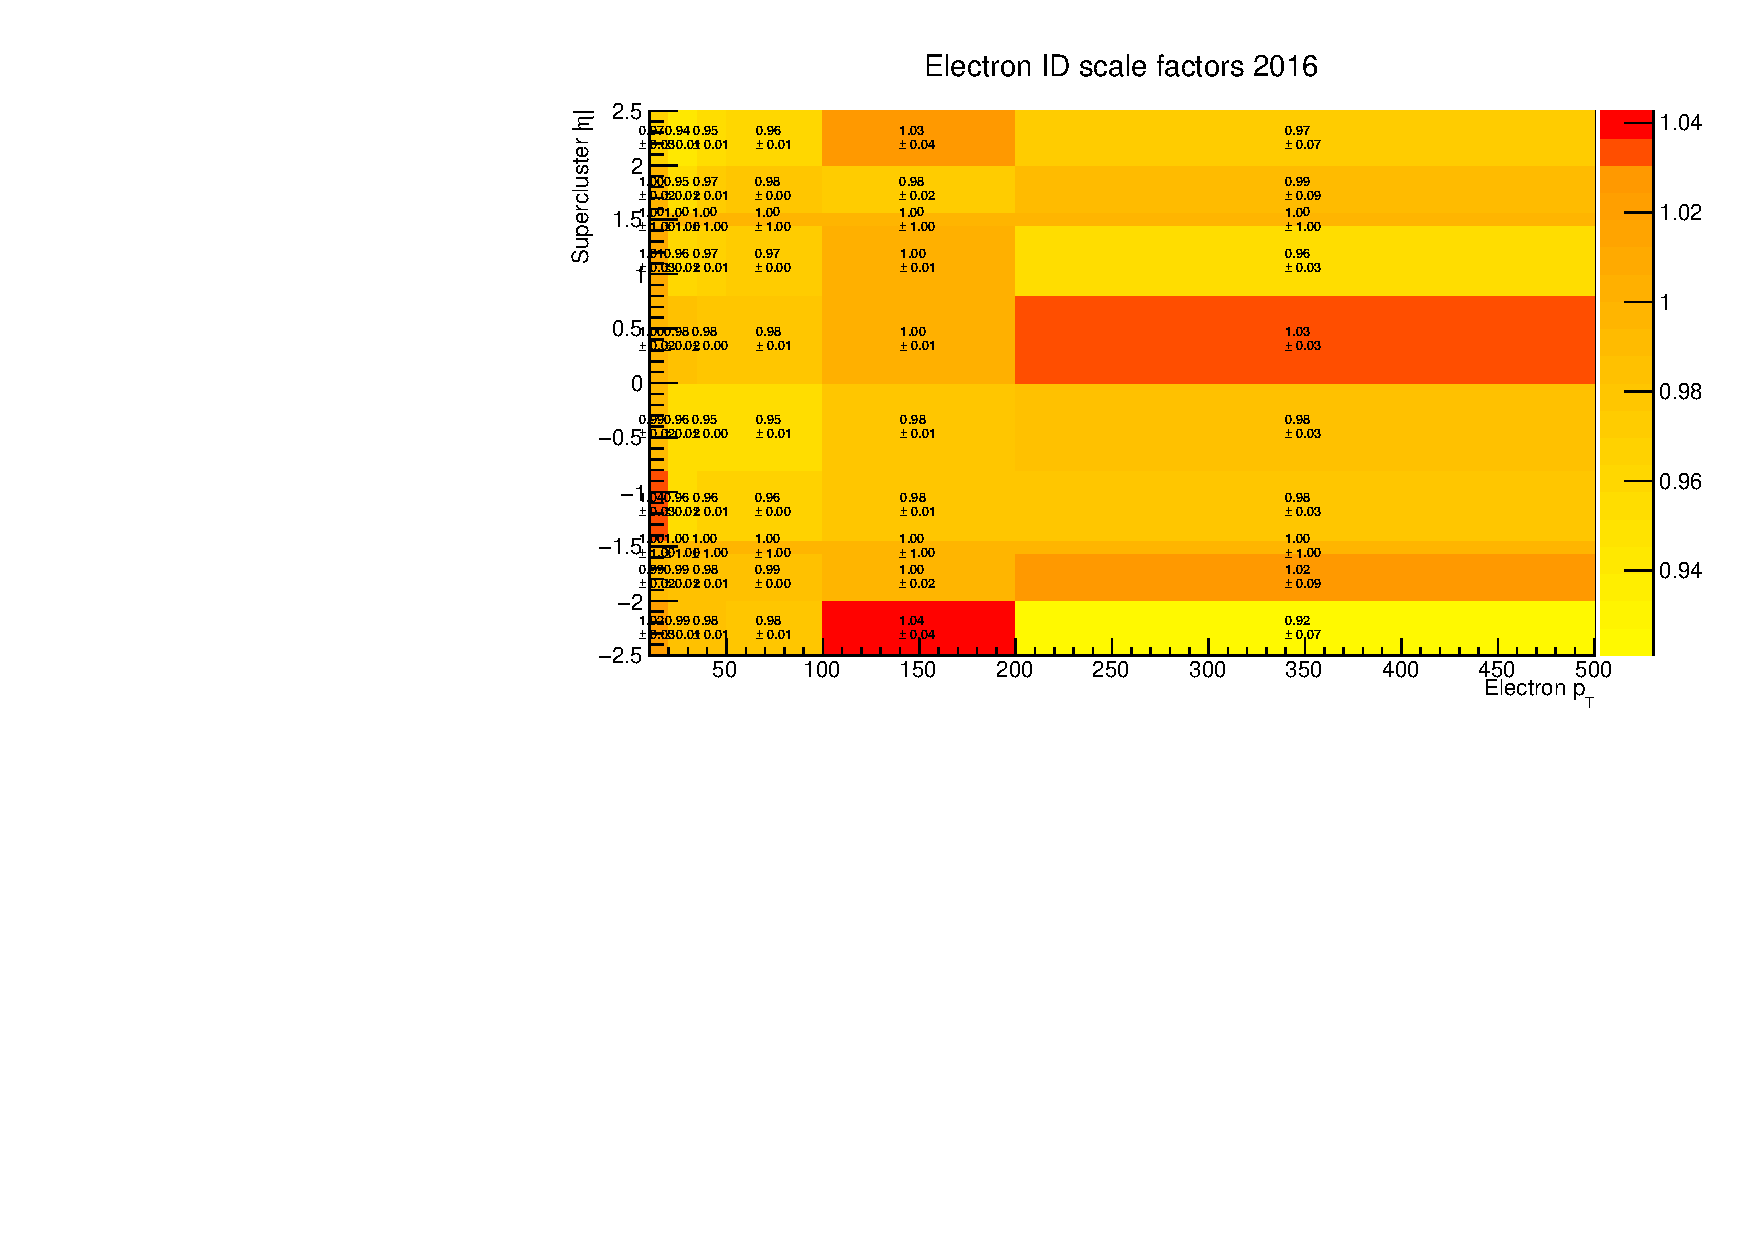
\includegraphics[width=0.5\textwidth]{Canvas_Electron_SF_2016_ID.pdf}
        \caption{Histogramme 2D des facteurs correctifs d'identification des électrons pour l'année 2016. L'abscisse est l'impulsion transverse \pt du jet considéré et l'ordonnée est sa pseudo-rapidité en valeur absolue $|\eta|$.}
    \end{center}
\end{figure}

\begin{figure}[H]
    \begin{center}
        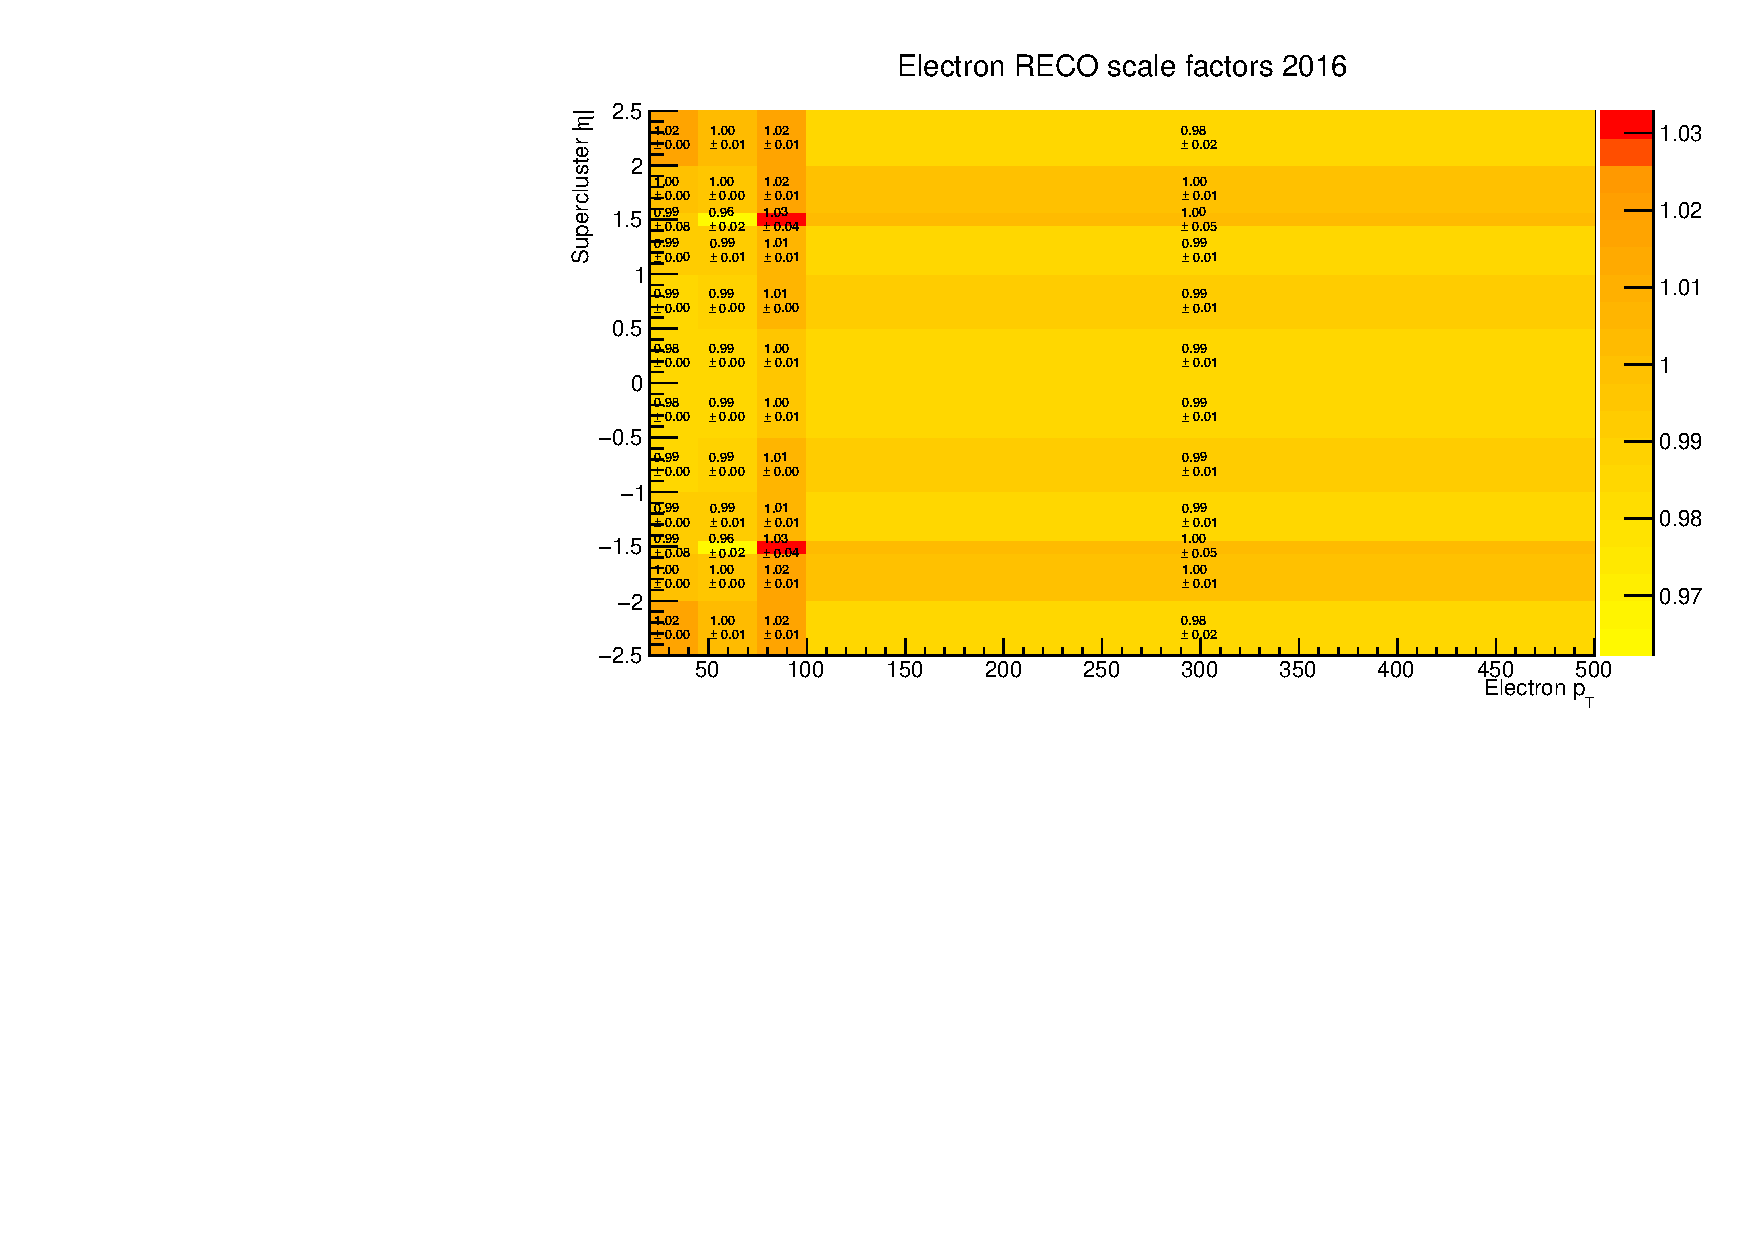
\includegraphics[width=0.5\textwidth]{Canvas_Electron_SF_2016_RECO.pdf}
        \caption{Histogramme 2D des facteurs correctifs de reconstructions des électrons pour l'année 2016. L'abscisse est l'impulsion transverse \pt du jet considéré et l'ordonnée est sa pseudo-rapidité en valeur absolue $|\eta|$.}
    \end{center}
\end{figure}

\begin{figure}[H]
    \begin{center}
        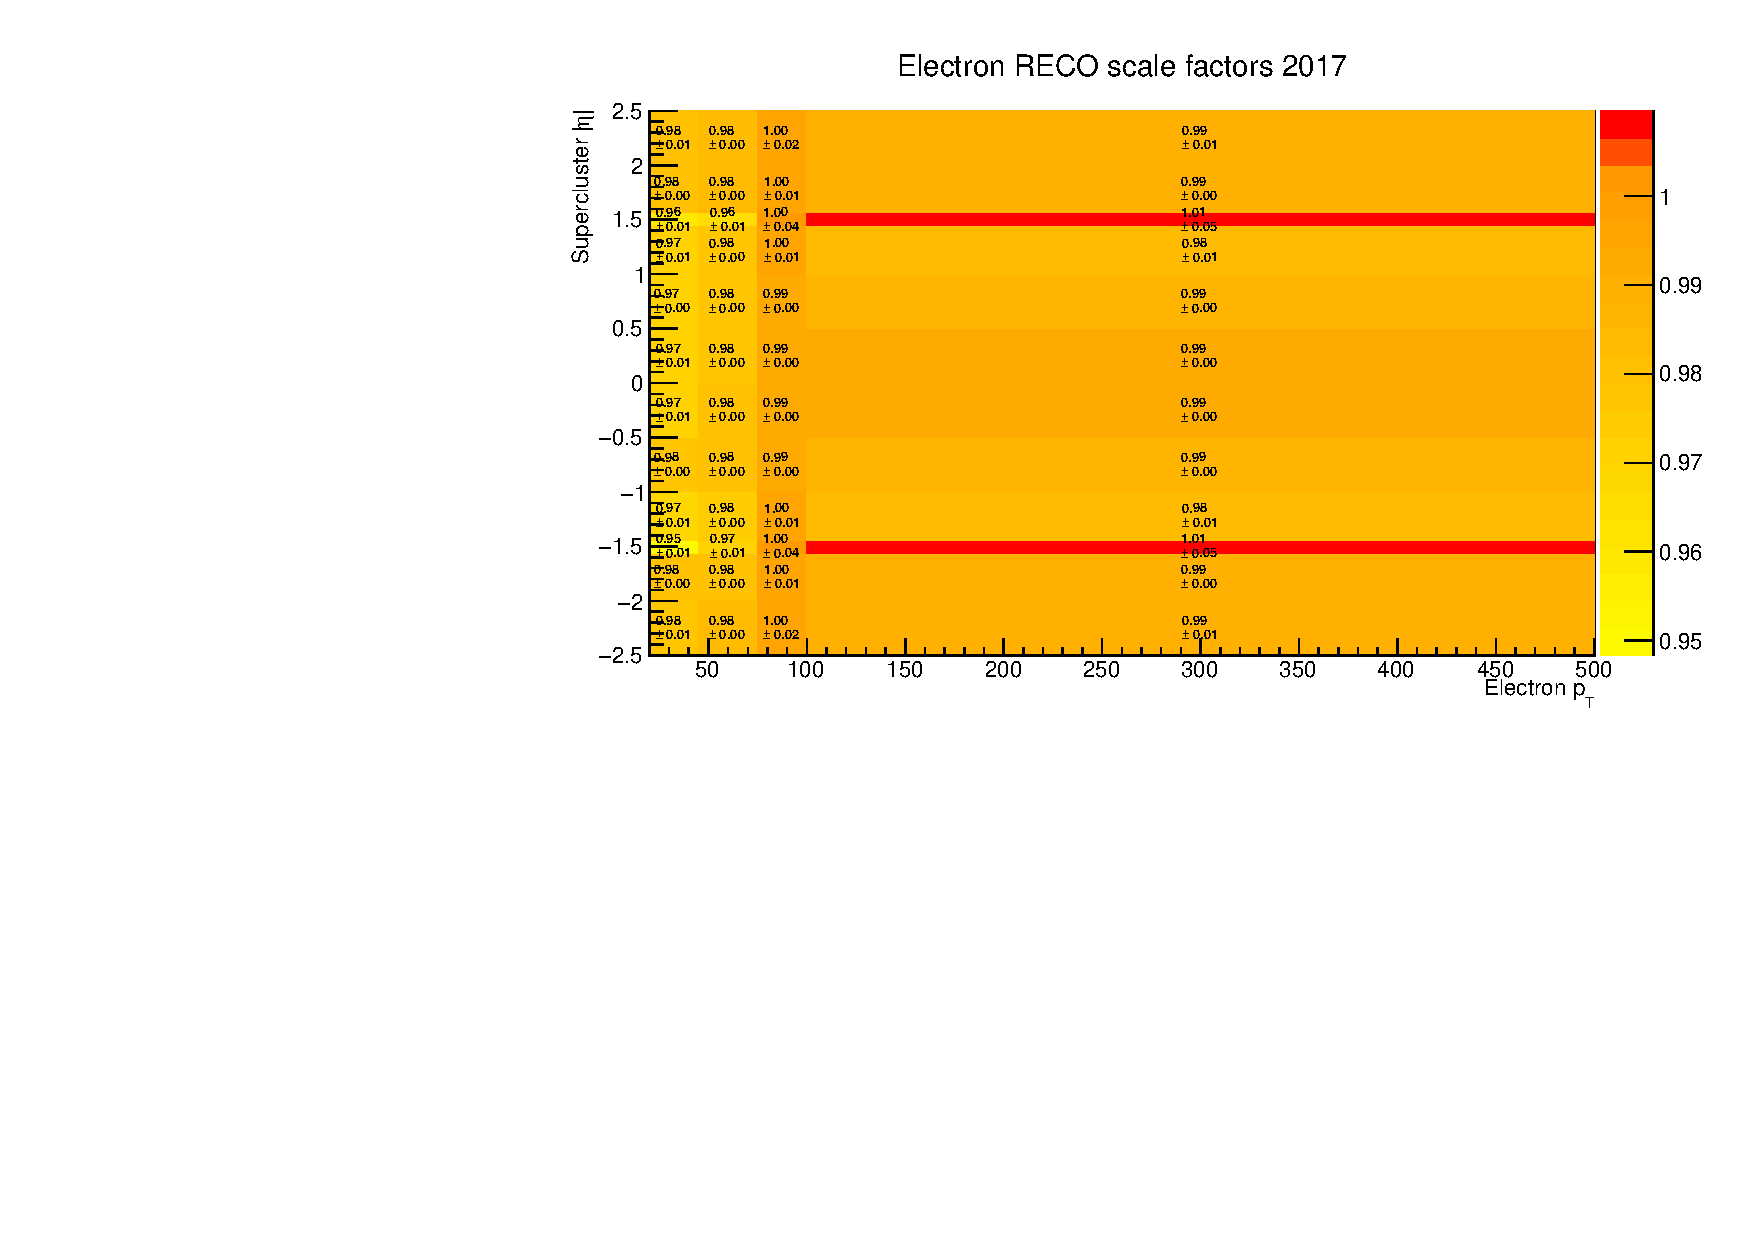
\includegraphics[width=0.5\textwidth]{Canvas_Electron_SF_2017_RECO.pdf}
        \caption{Histogramme 2D des facteurs correctifs de reconstructions des électrons pour l'année 2017. L'abscisse est l'impulsion transverse \pt du jet considéré et l'ordonnée est sa pseudo-rapidité en valeur absolue $|\eta|$.}
    \end{center}
\end{figure}

\begin{figure}[H]
    \begin{center}
        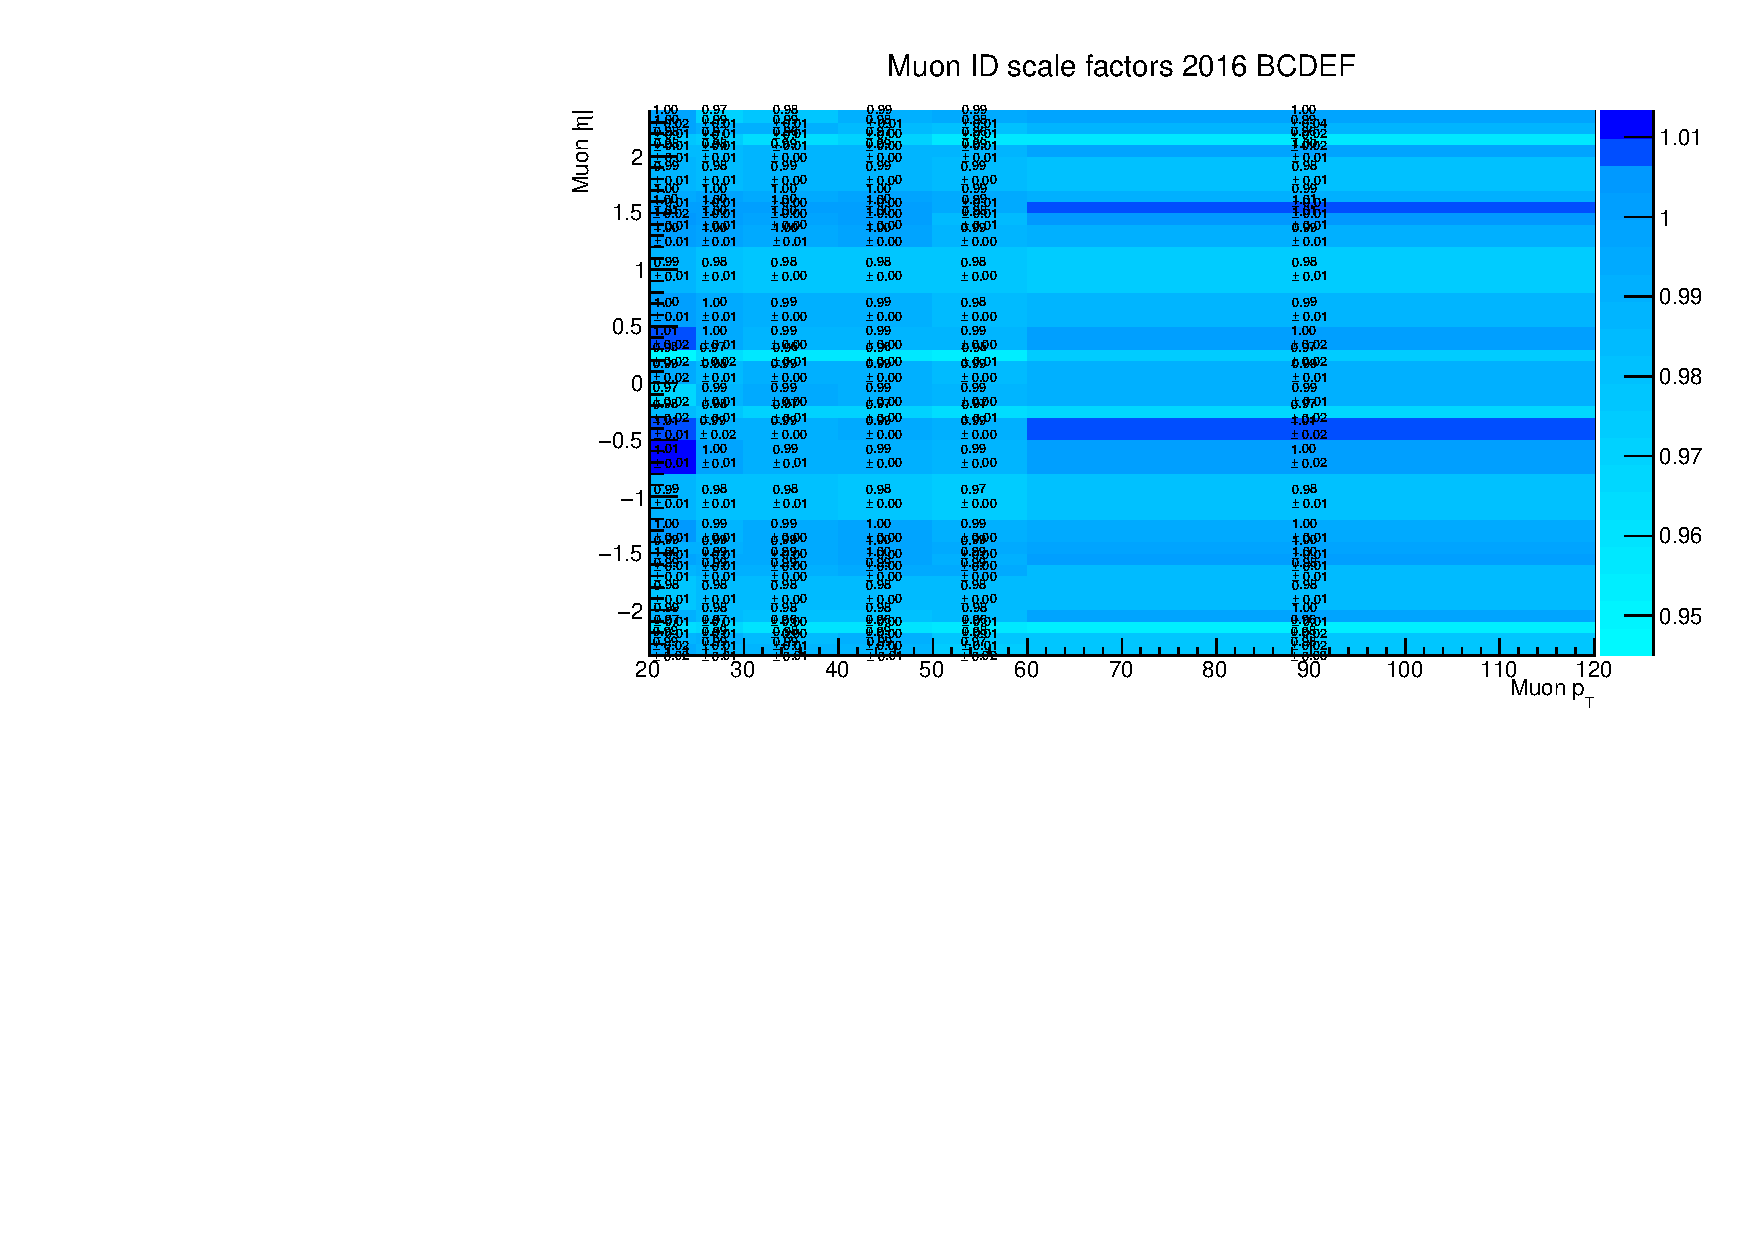
\includegraphics[width=0.5\textwidth]{Canvas_Muon_SF_2016_ID_BCDEF.pdf}
        \caption{Histogramme 2D des facteurs correctifs d'identification des muons pour l'année 2016 pour les ères de données B,C,D,E et F. L'abscisse est l'impulsion transverse \pt du jet considéré et l'ordonnée est sa pseudo-rapidité en valeur absolue $|\eta|$.}
    \end{center}
\end{figure}

\begin{figure}[H]
    \begin{center}
        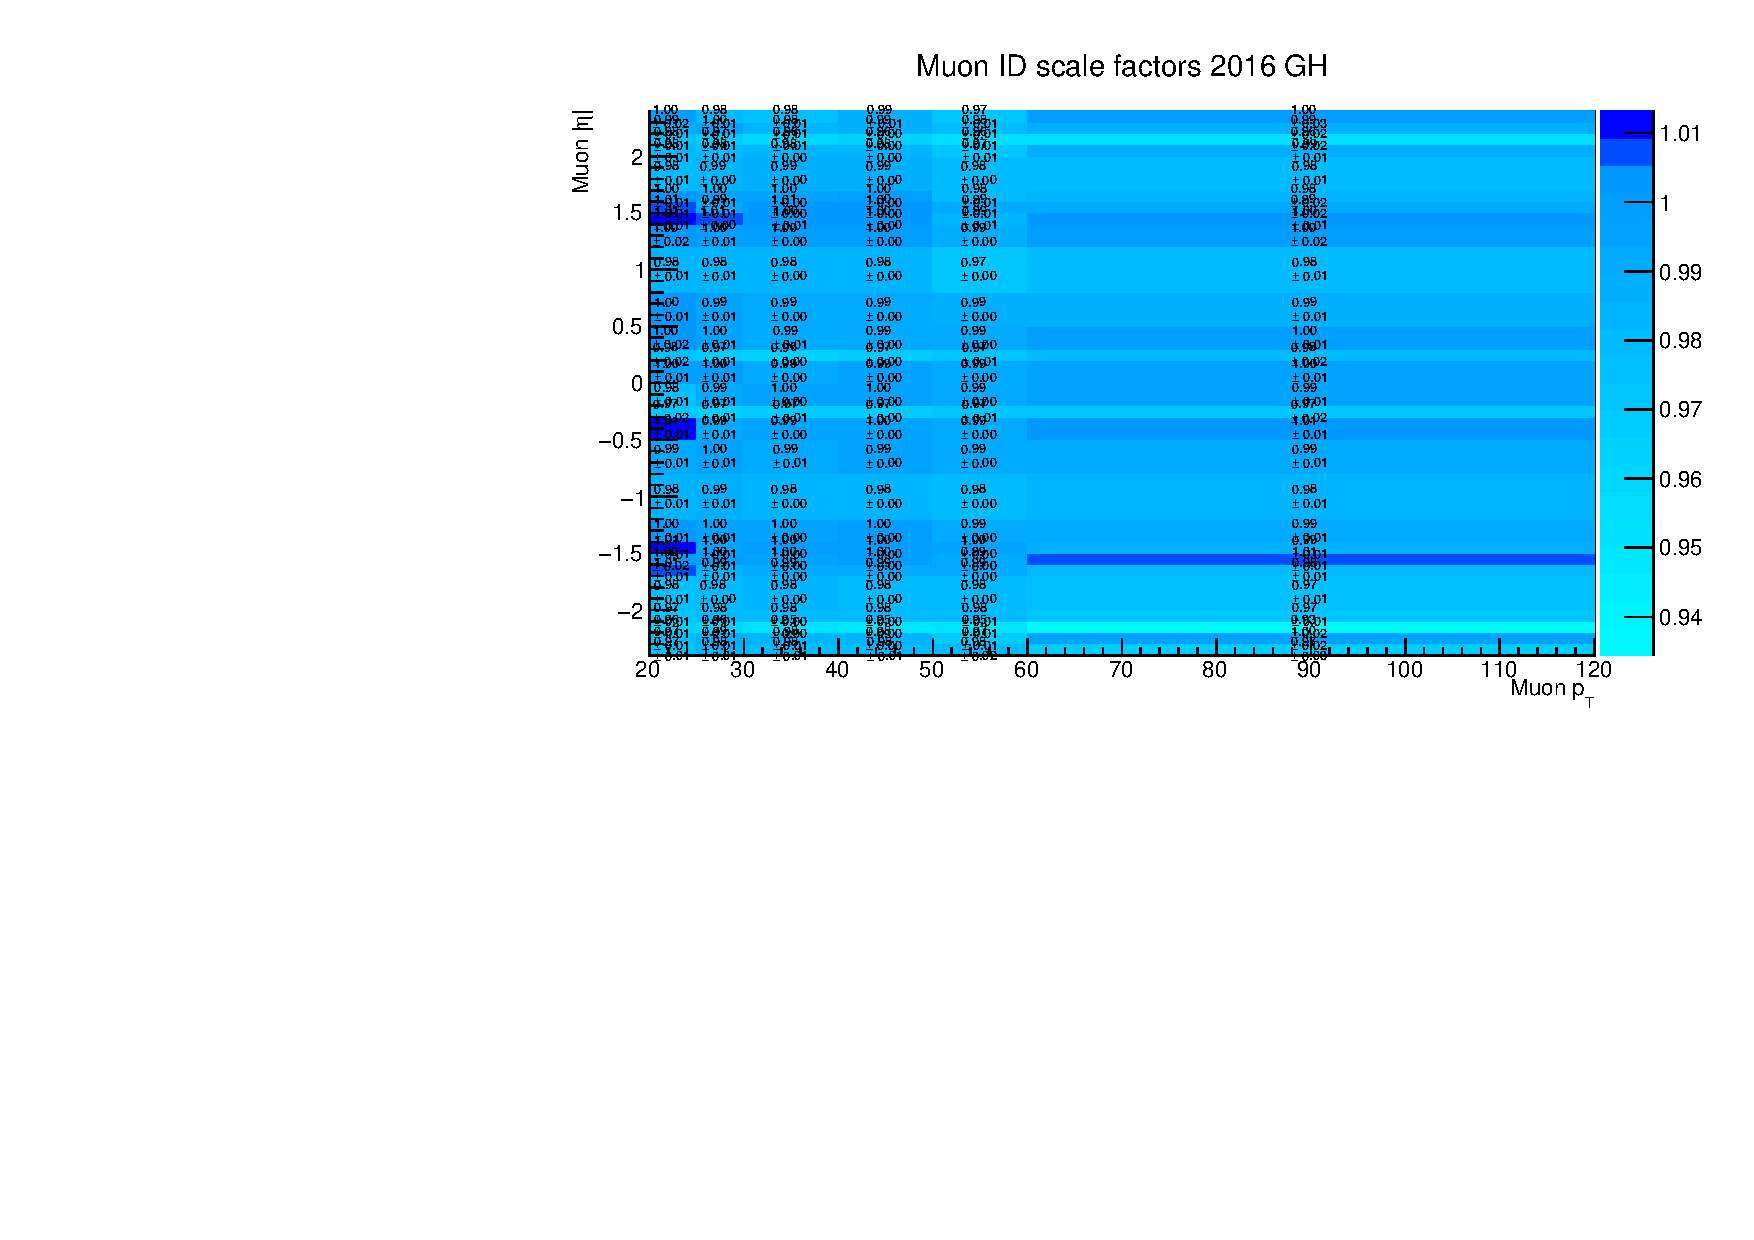
\includegraphics[width=0.5\textwidth]{Canvas_Muon_SF_2016_ID_GH.pdf}
        \caption{Histogramme 2D des facteurs correctifs d'identification des muons pour l'année 2016 pour les ères de données G et H. L'abscisse est l'impulsion transverse \pt du jet considéré et l'ordonnée est sa pseudo-rapidité en valeur absolue $|\eta|$.}
    \end{center}
\end{figure}



\begin{figure}[H]
    \begin{center}
        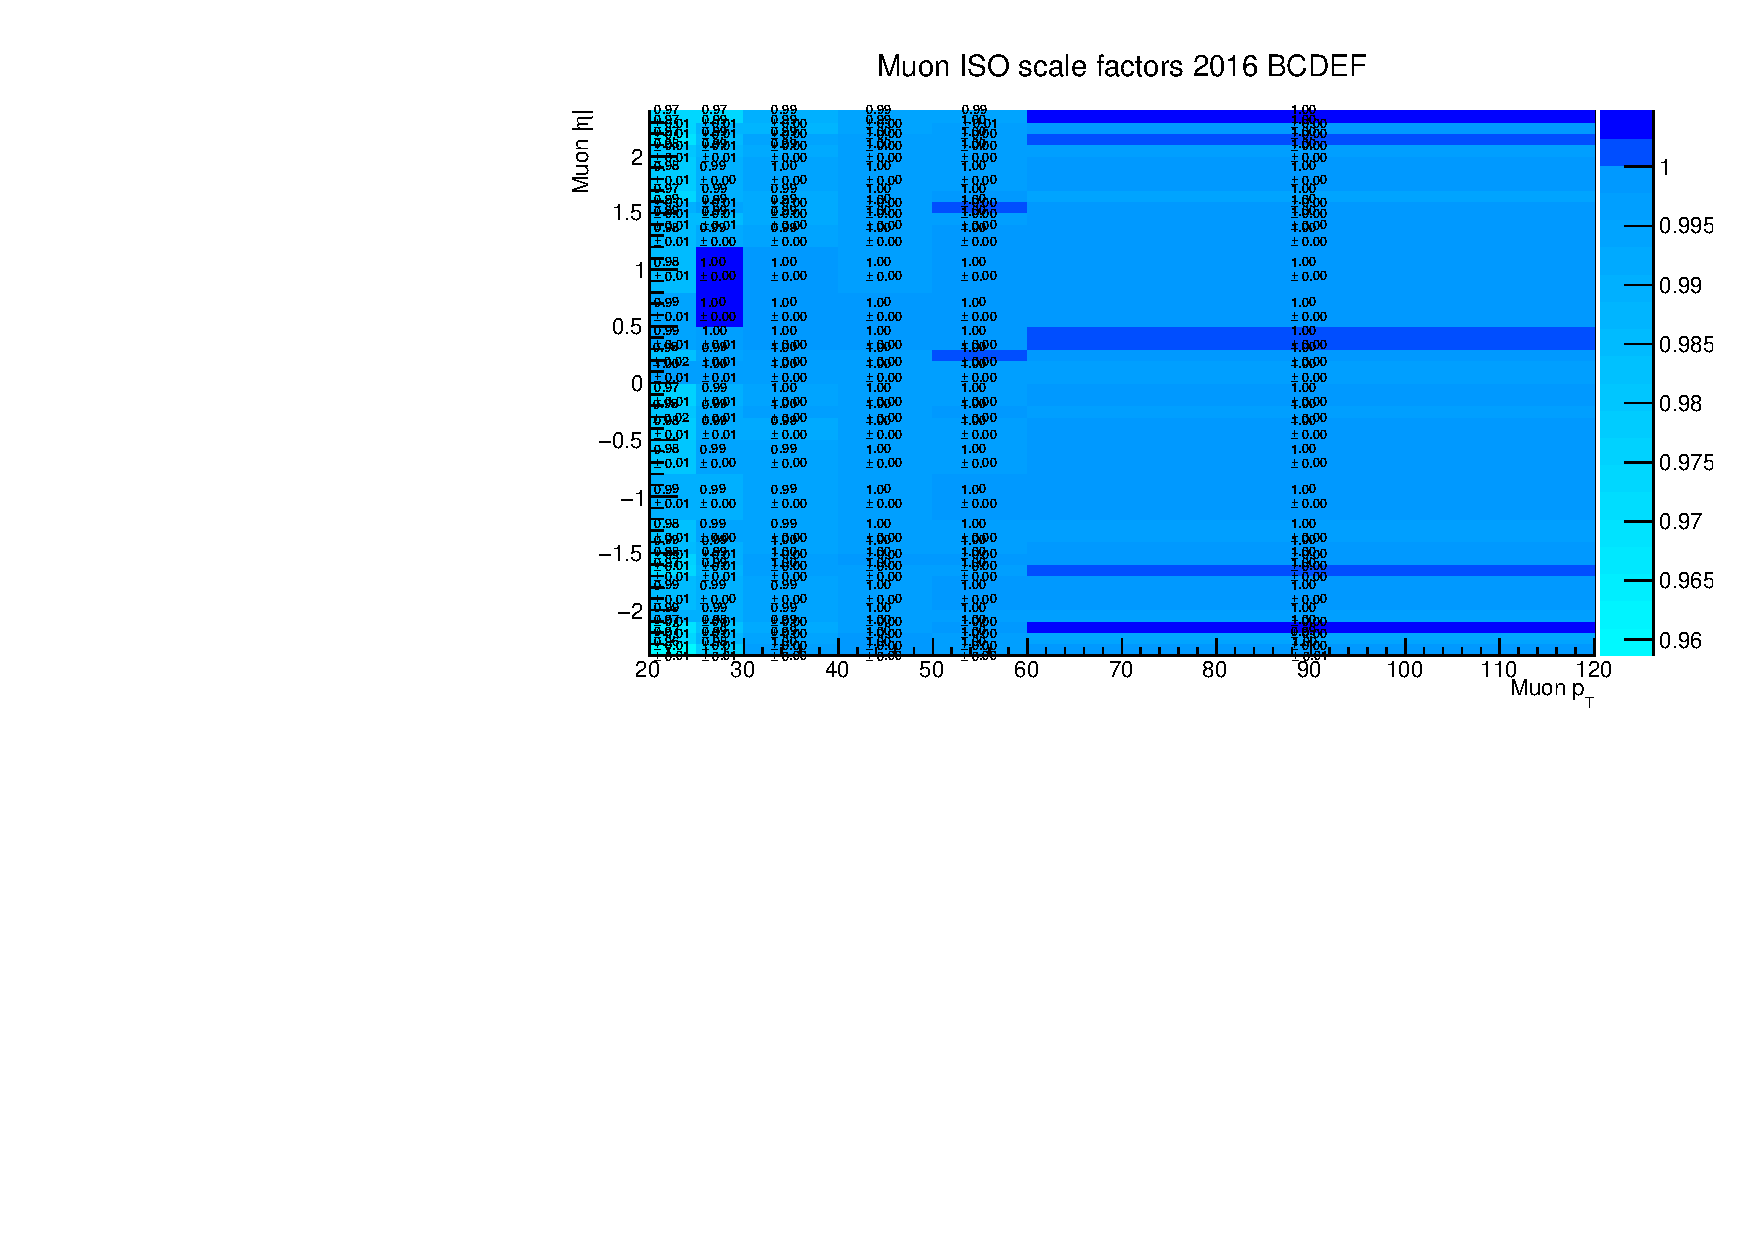
\includegraphics[width=0.5\textwidth]{Canvas_Muon_SF_2016_ISO_BCDEF.pdf}
        \caption{Histogramme 2D des facteurs correctifs d'isolation des muons pour l'année 2016 pour les ères de données B,C,D,E et F. L'abscisse est l'impulsion transverse \pt du jet considéré et l'ordonnée est sa pseudo-rapidité en valeur absolue $|\eta|$.}
    \end{center}
\end{figure}

\begin{figure}[H]
    \begin{center}
        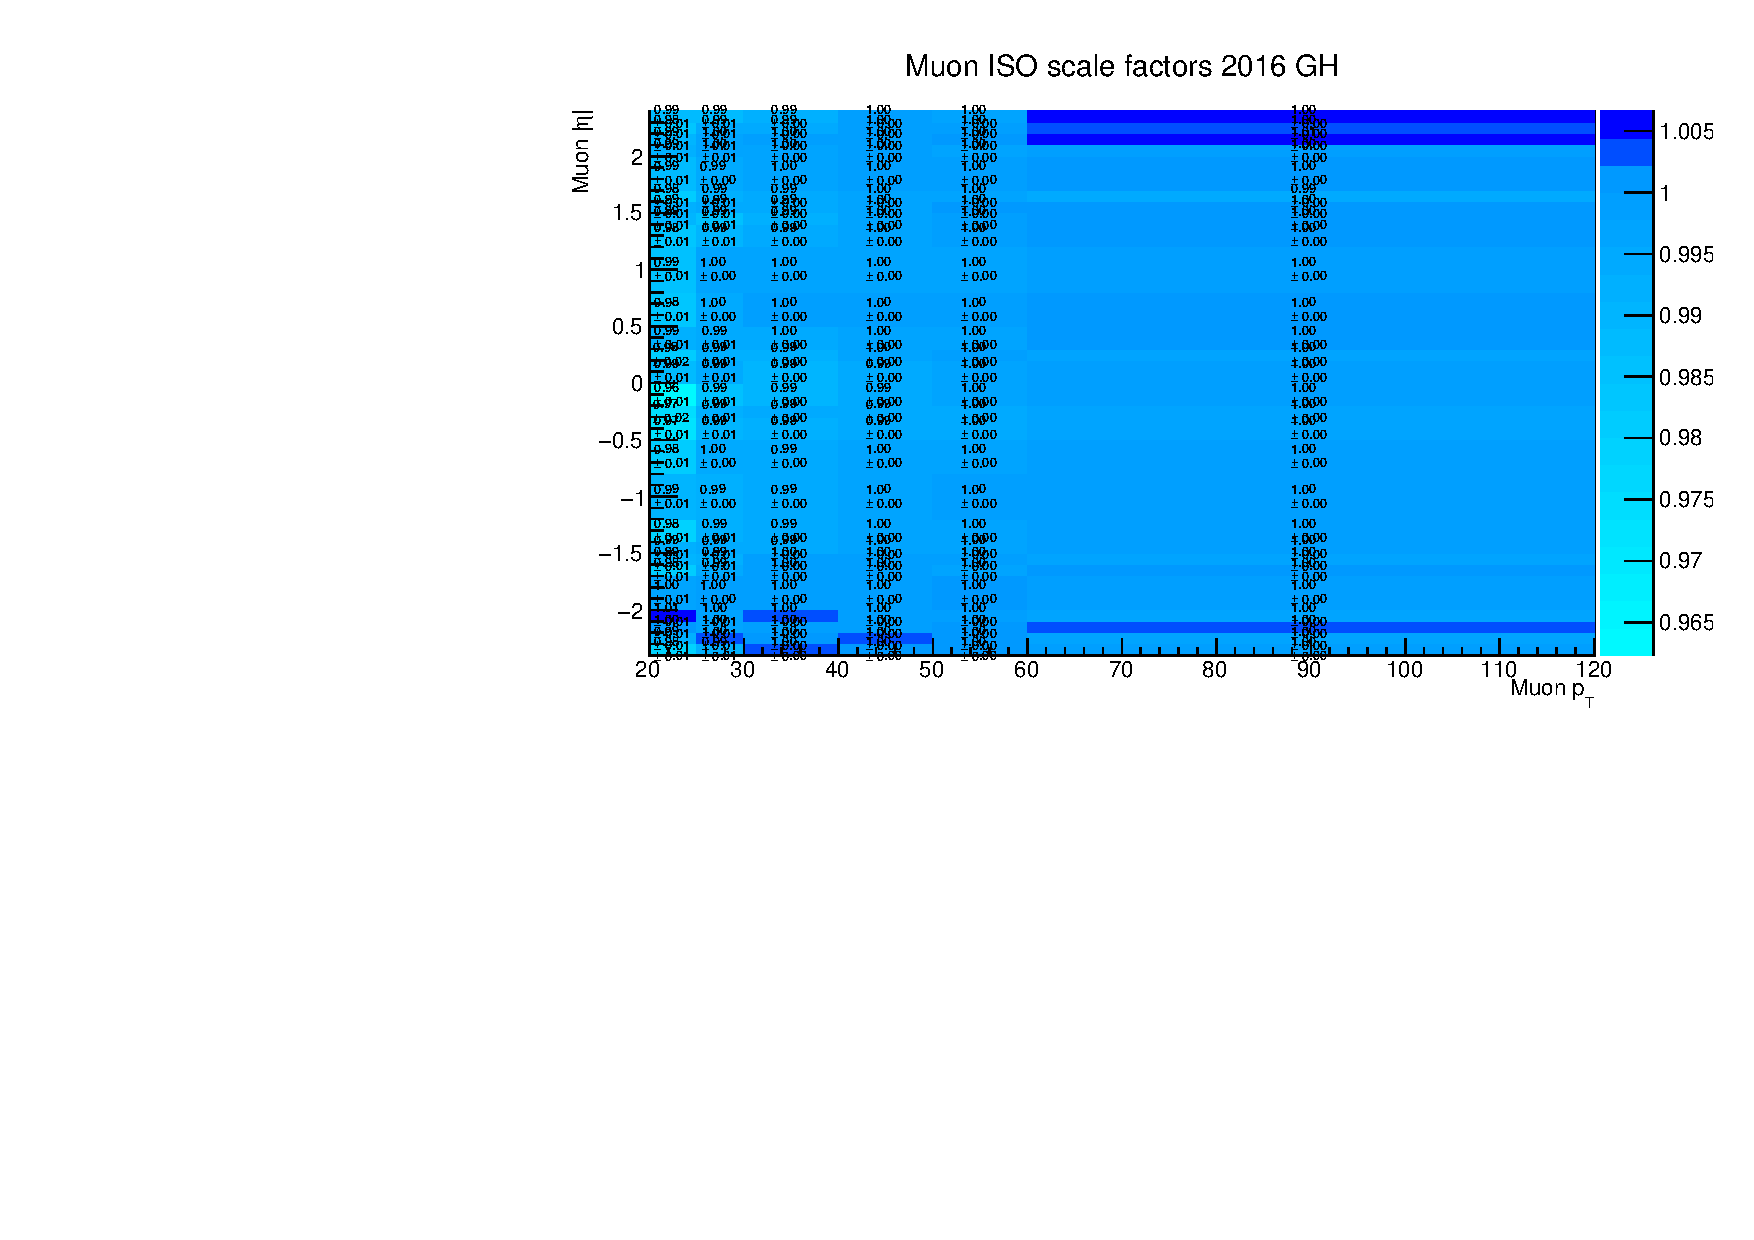
\includegraphics[width=0.5\textwidth]{Canvas_Muon_SF_2016_ISO_GH.pdf}
        \caption{Histogramme 2D des facteurs correctifs d'isolation des muons pour l'année 2016 pour les ères de données G et H. L'abscisse est l'impulsion transverse \pt du jet considéré et l'ordonnée est sa pseudo-rapidité en valeur absolue $|\eta|$.}
    \end{center}
\end{figure}


\begin{figure}[H]
    \begin{center}
        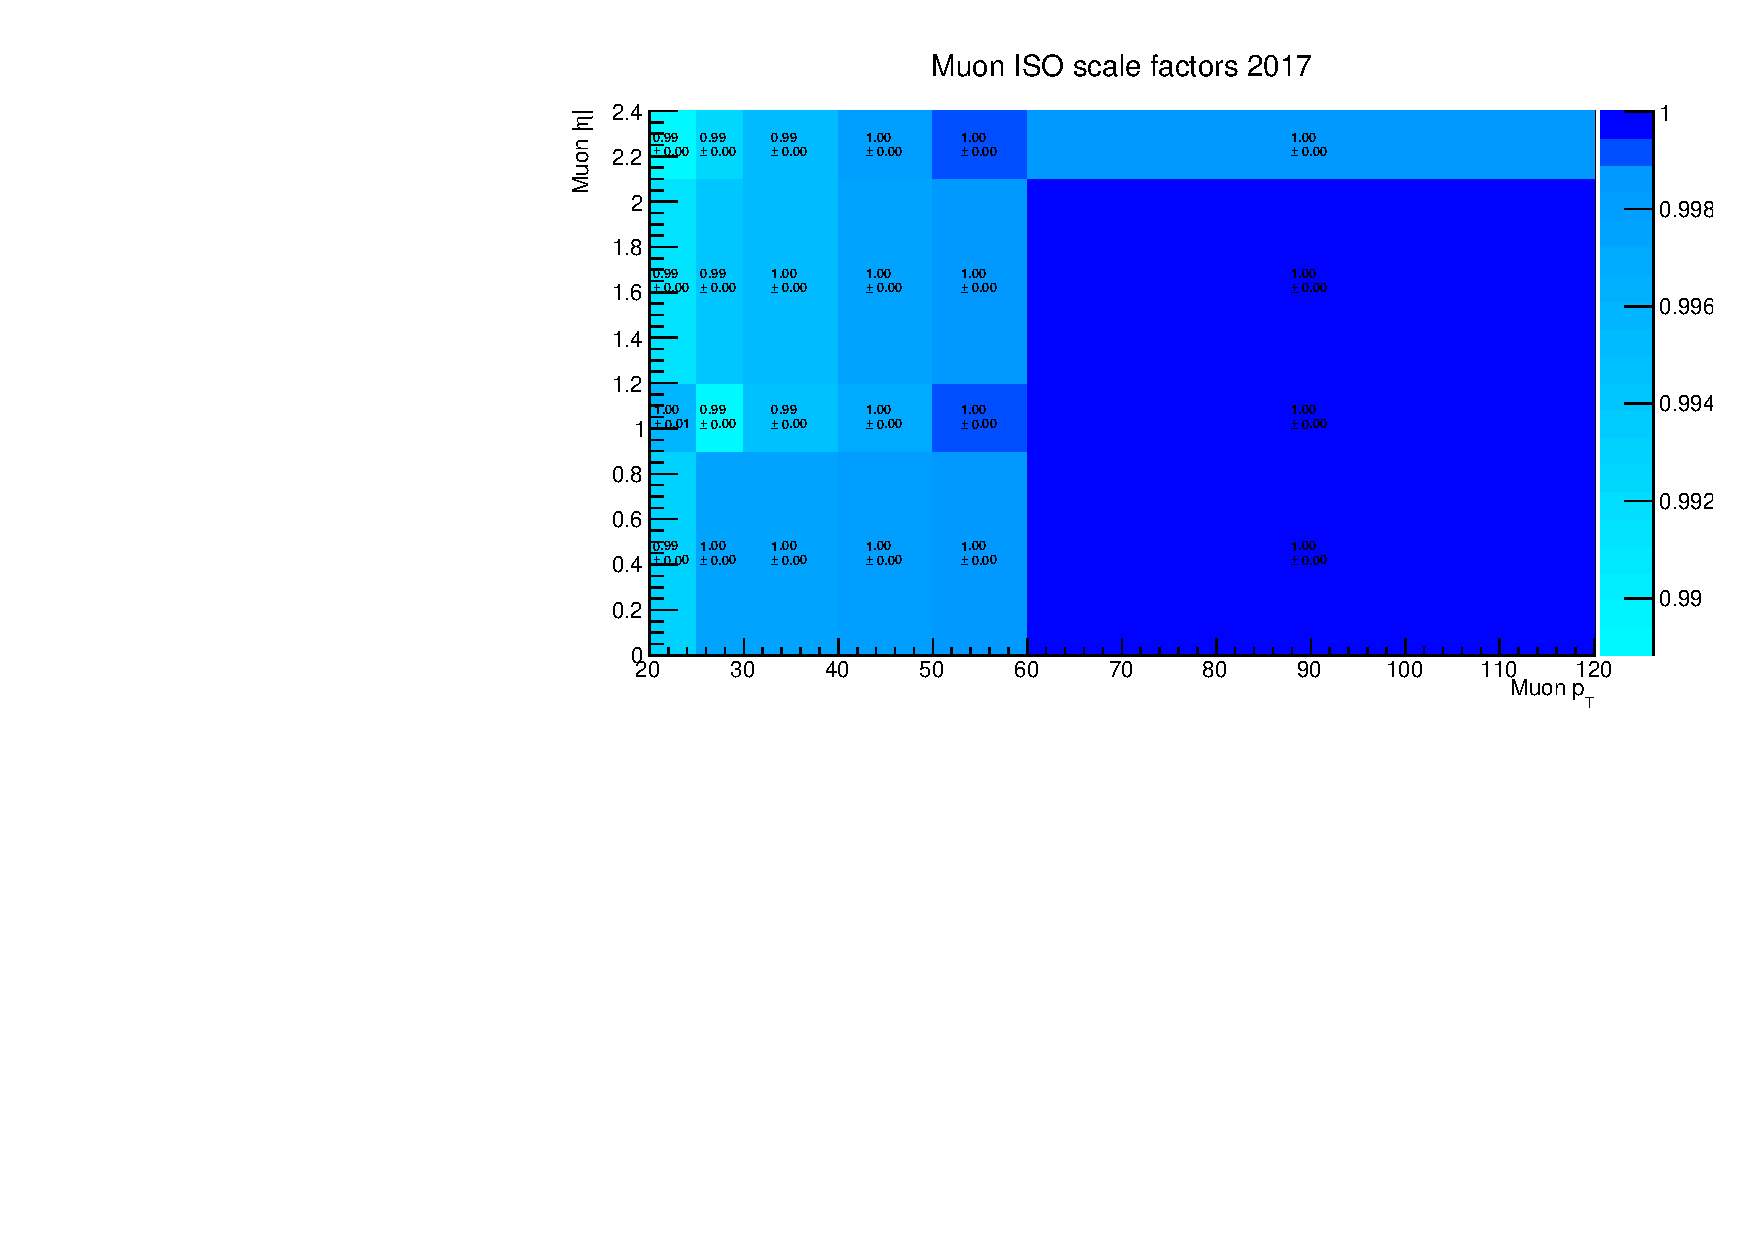
\includegraphics[width=0.5\textwidth]{Canvas_Muon_SF_2017_ISO.pdf}
        \caption{Histogramme 2D des facteurs correctifs d'isolation des muons pour l'année 2017. L'abscisse est l'impulsion transverse \pt du jet considéré et l'ordonnée est sa pseudo-rapidité en valeur absolue $|\eta|$.}
    \end{center}
\end{figure}




\subsection{$b$-, $c$-, light-jets tagging}\label{app:sfb}

\begin{figure}[H]
    \begin{center}
        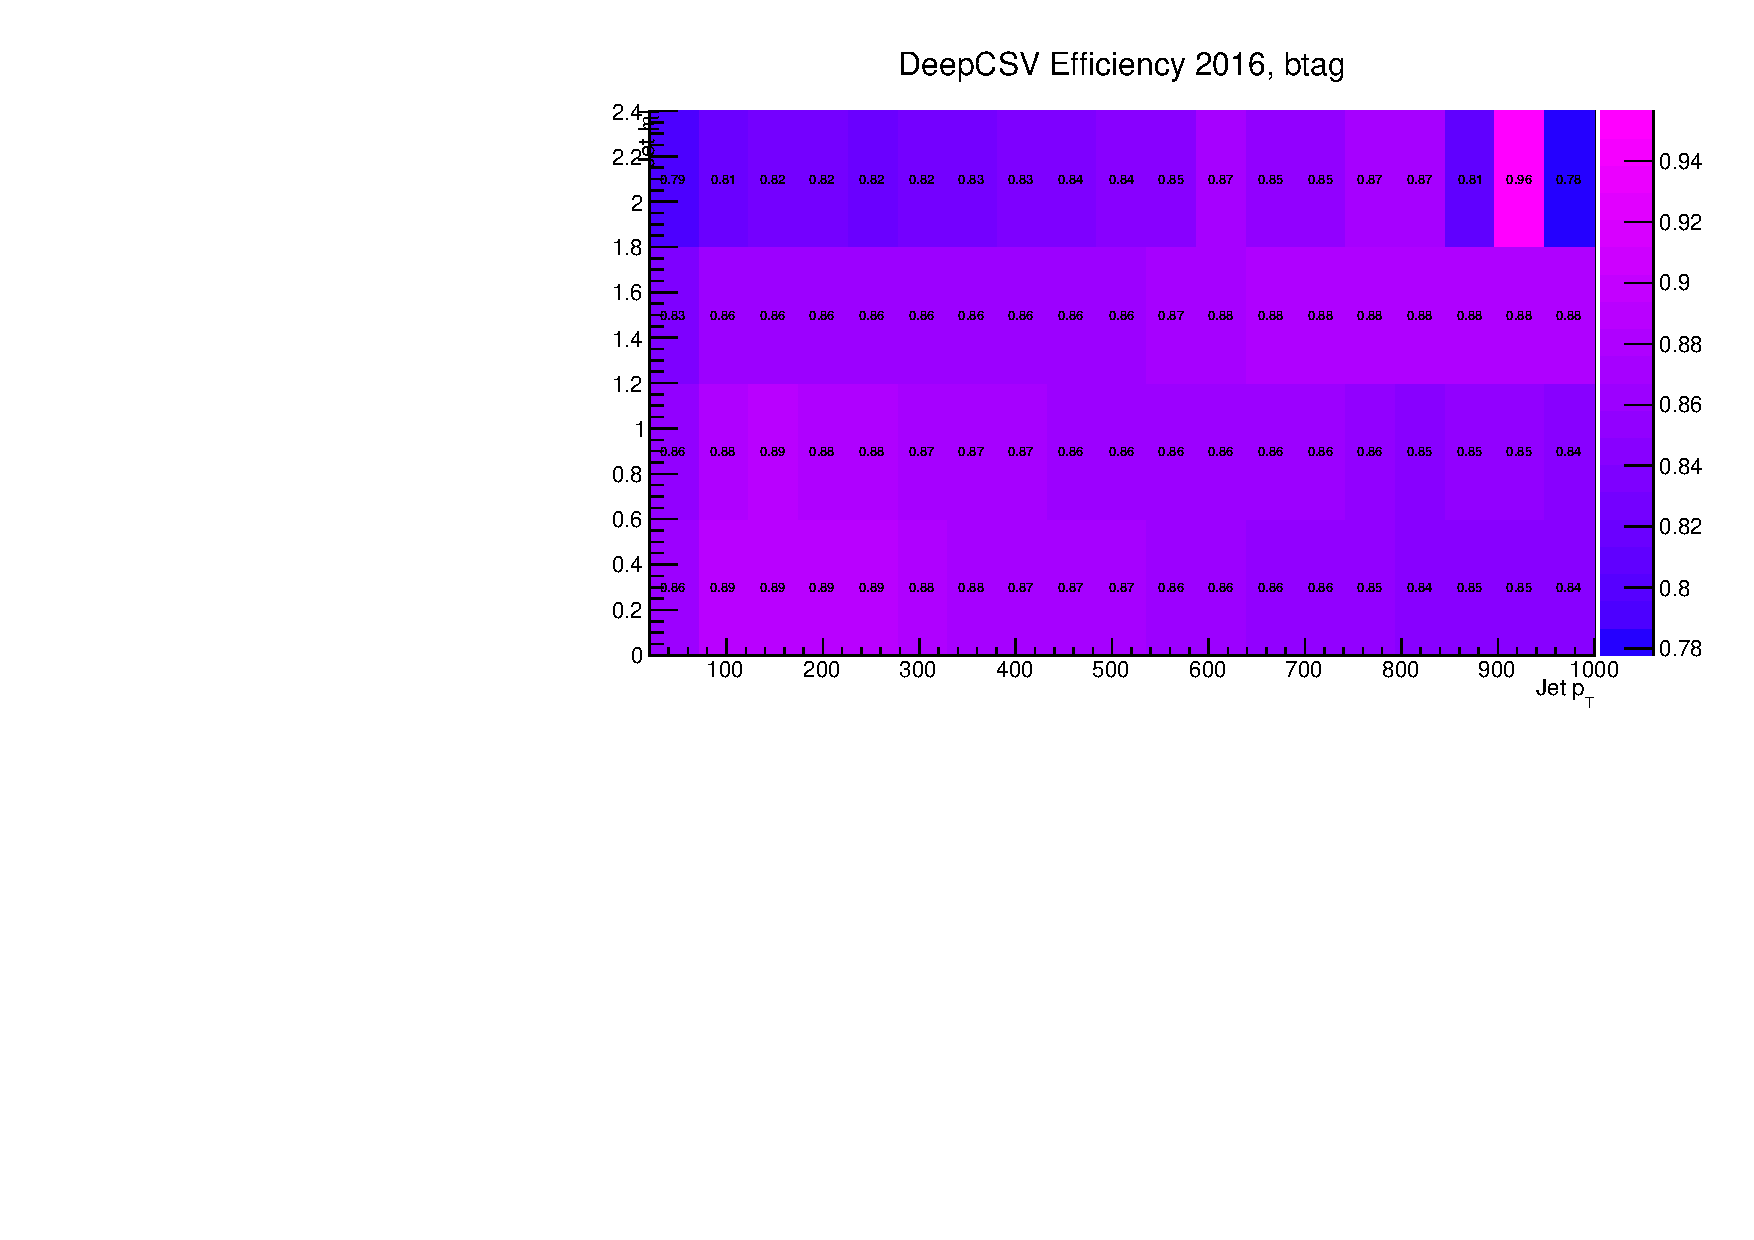
\includegraphics[width=0.5\textwidth]{Canvas_DeepCSV_SF_2016_btag.pdf}
        \caption{Histogramme 2D des facteurs correctifs pour l'efficacité de l'étiquetage \Pbottom{} avec l'algorithme DeepCSV. L'abscisse est l'impulsion transverse \pt du jet considéré et l'ordonnée est sa pseudo-rapidité en valeur absolue $|\eta|$.}
    \end{center}
\end{figure}


\begin{figure}[H]
    \begin{center}
        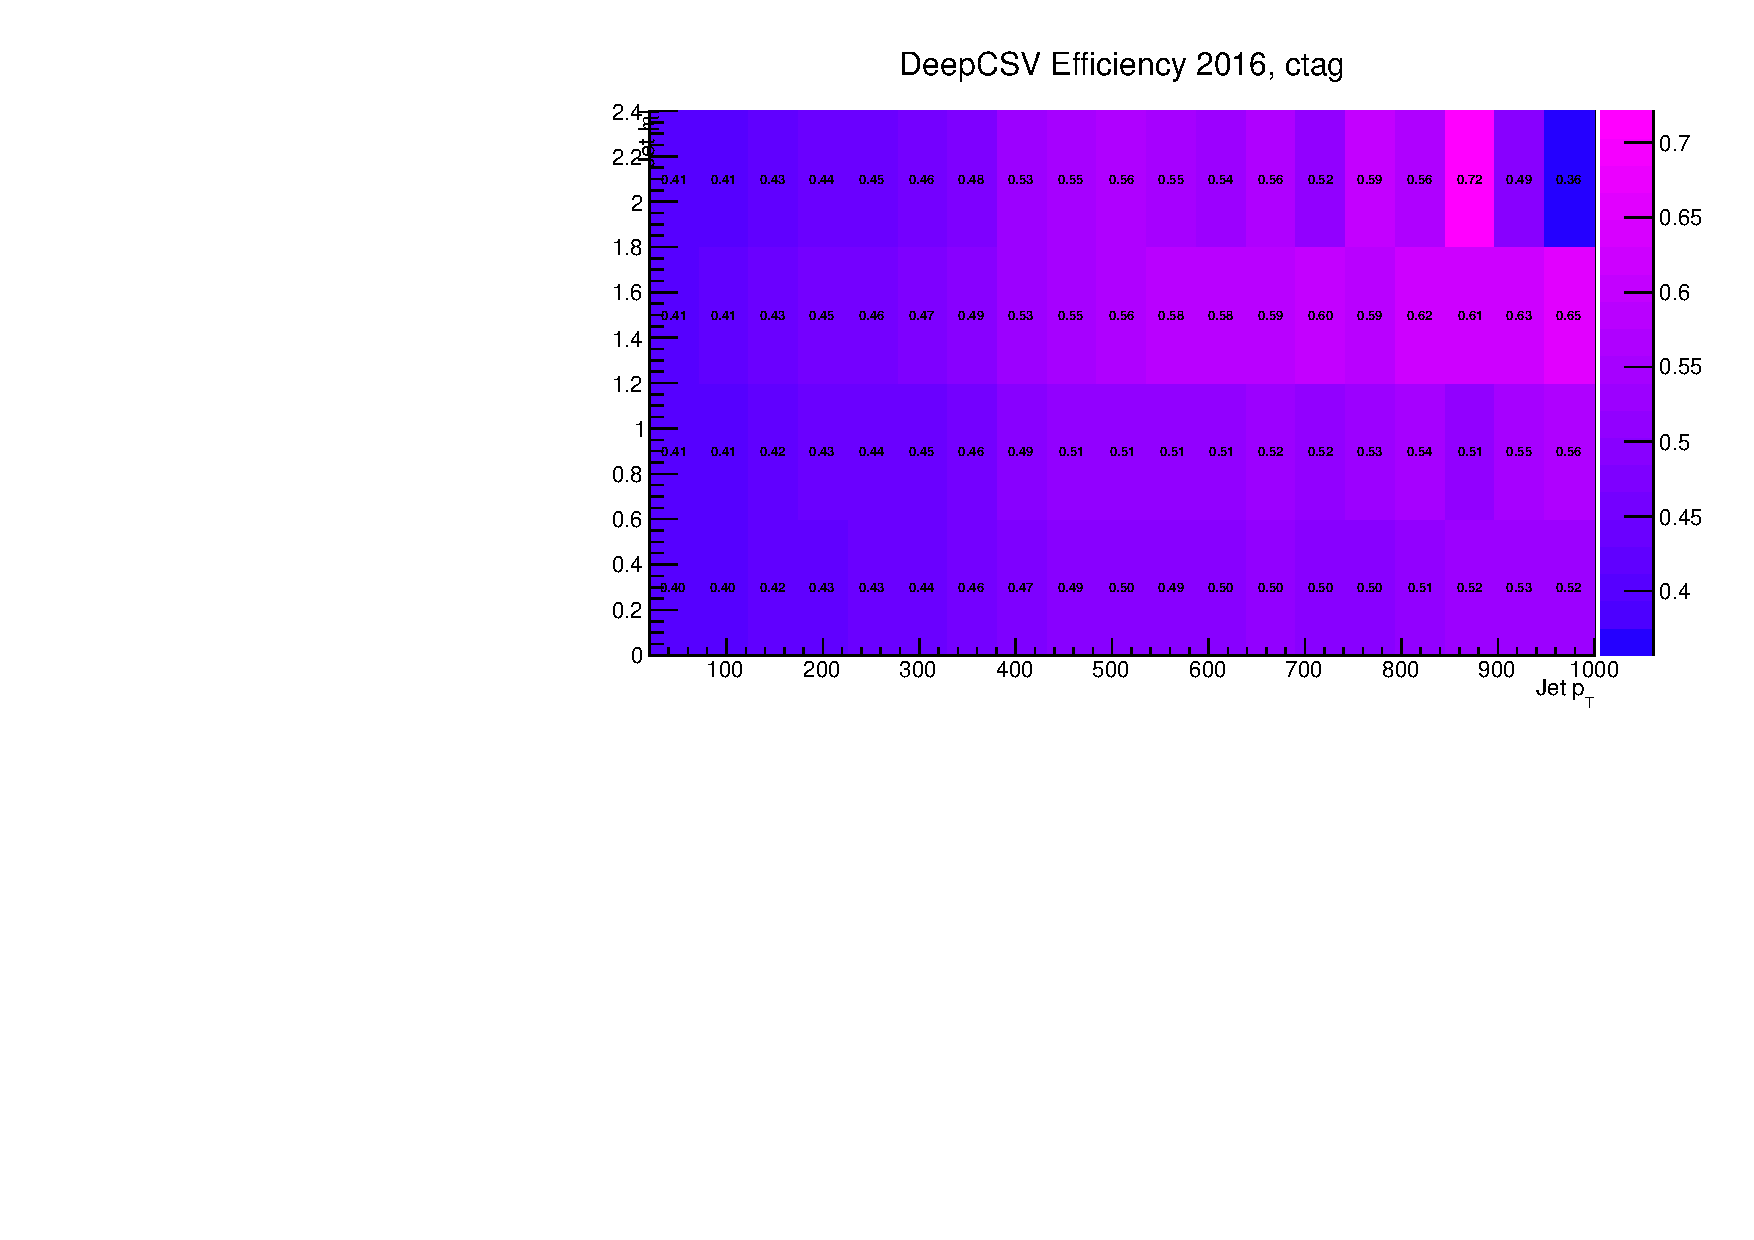
\includegraphics[width=0.5\textwidth]{Canvas_DeepCSV_SF_2016_ctag.pdf}
        \caption{Histogramme 2D des facteurs correctifs pour l'efficacité de l'étiquetage \Pcharm{} avec l'algorithme DeepCSV. L'abscisse est l'impulsion transverse \pt du jet considéré et l'ordonnée est sa pseudo-rapidité en valeur absolue $|\eta|$.}
    \end{center}
\end{figure}

\begin{figure}[H]
    \begin{center}
        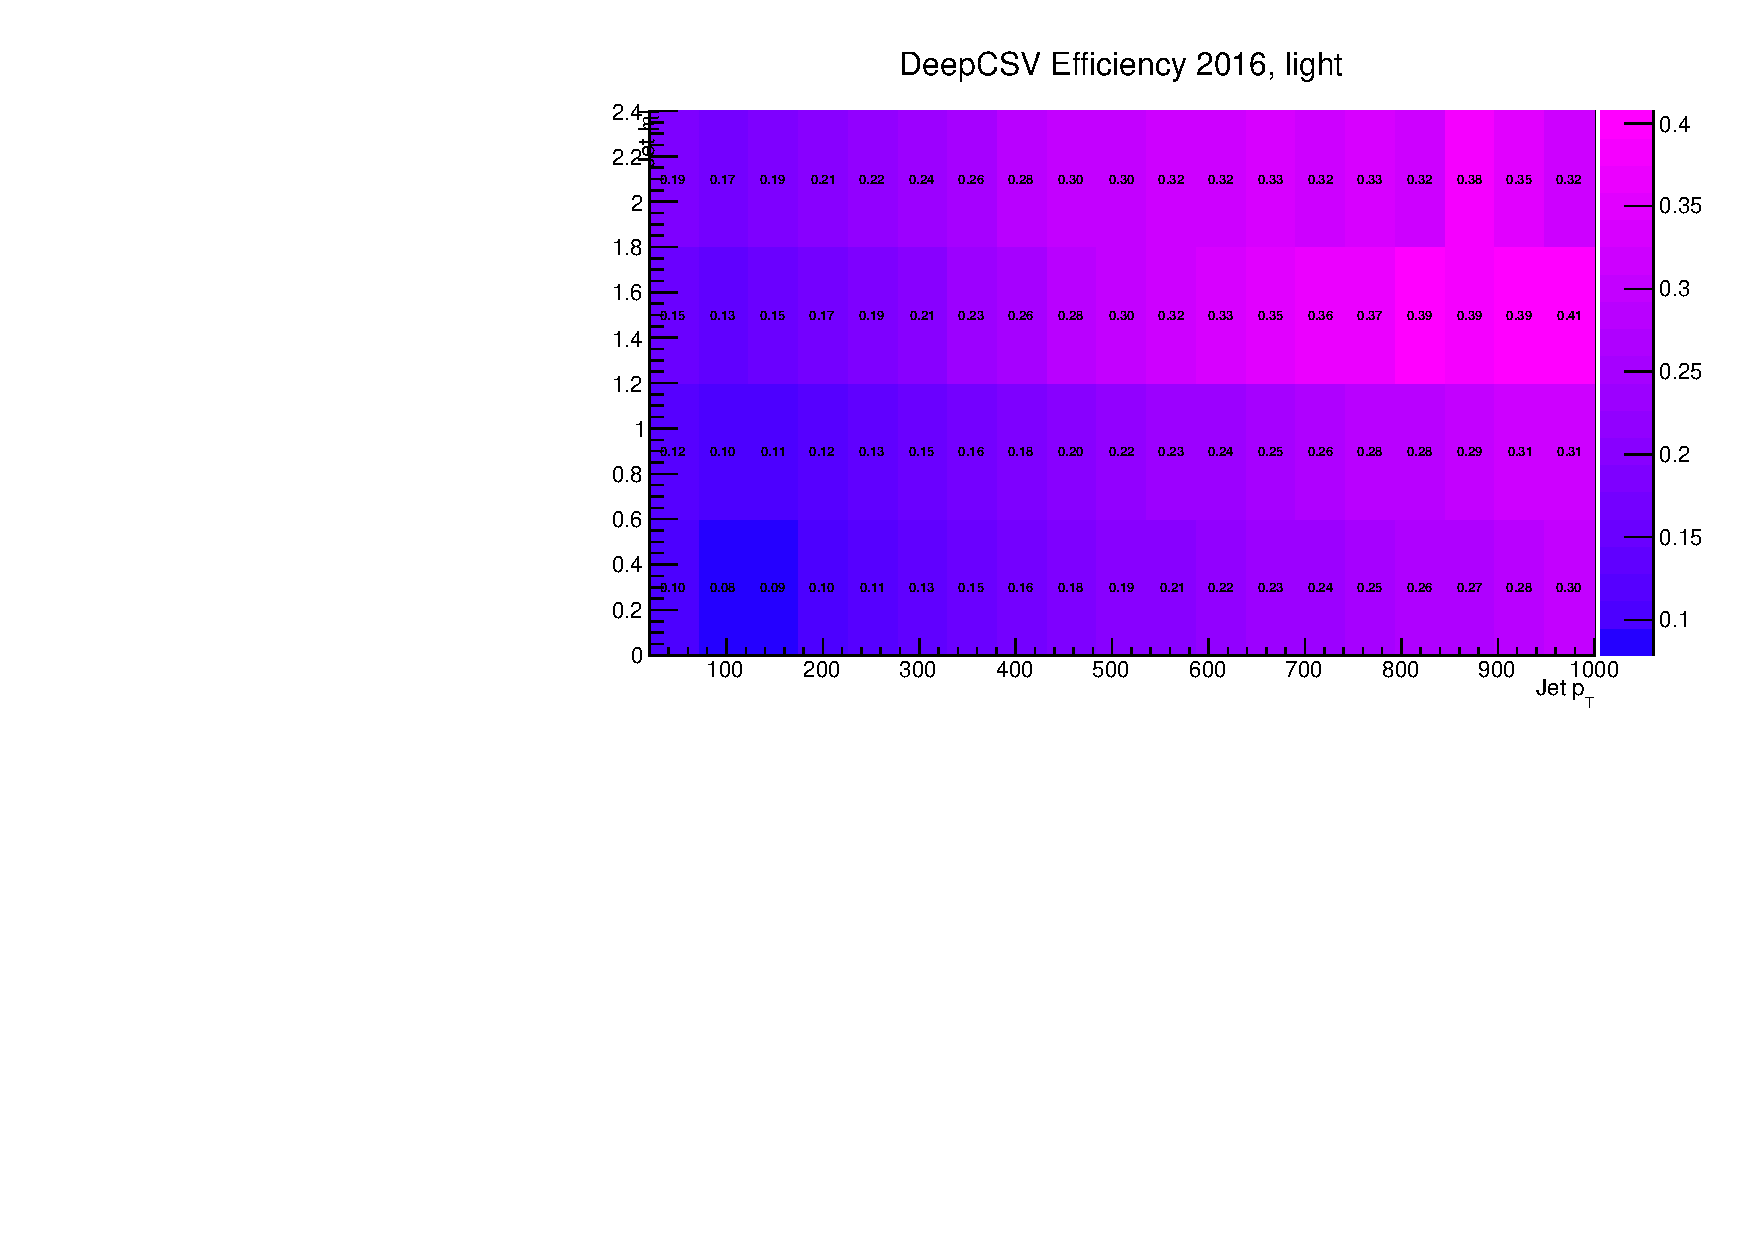
\includegraphics[width=0.5\textwidth]{Canvas_DeepCSV_SF_2016_light.pdf}
        \caption{Histogramme 2D des facteurs correctifs pour l'efficacité de l'étiquetage des lights jets avec l'algorithme DeepCSV. L'abscisse est l'impulsion transverse \pt du jet considéré et l'ordonnée est sa pseudo-rapidité en valeur absolue $|\eta|$.}
    \end{center}
\end{figure}



\begin{figure}[H]
    \begin{center}
        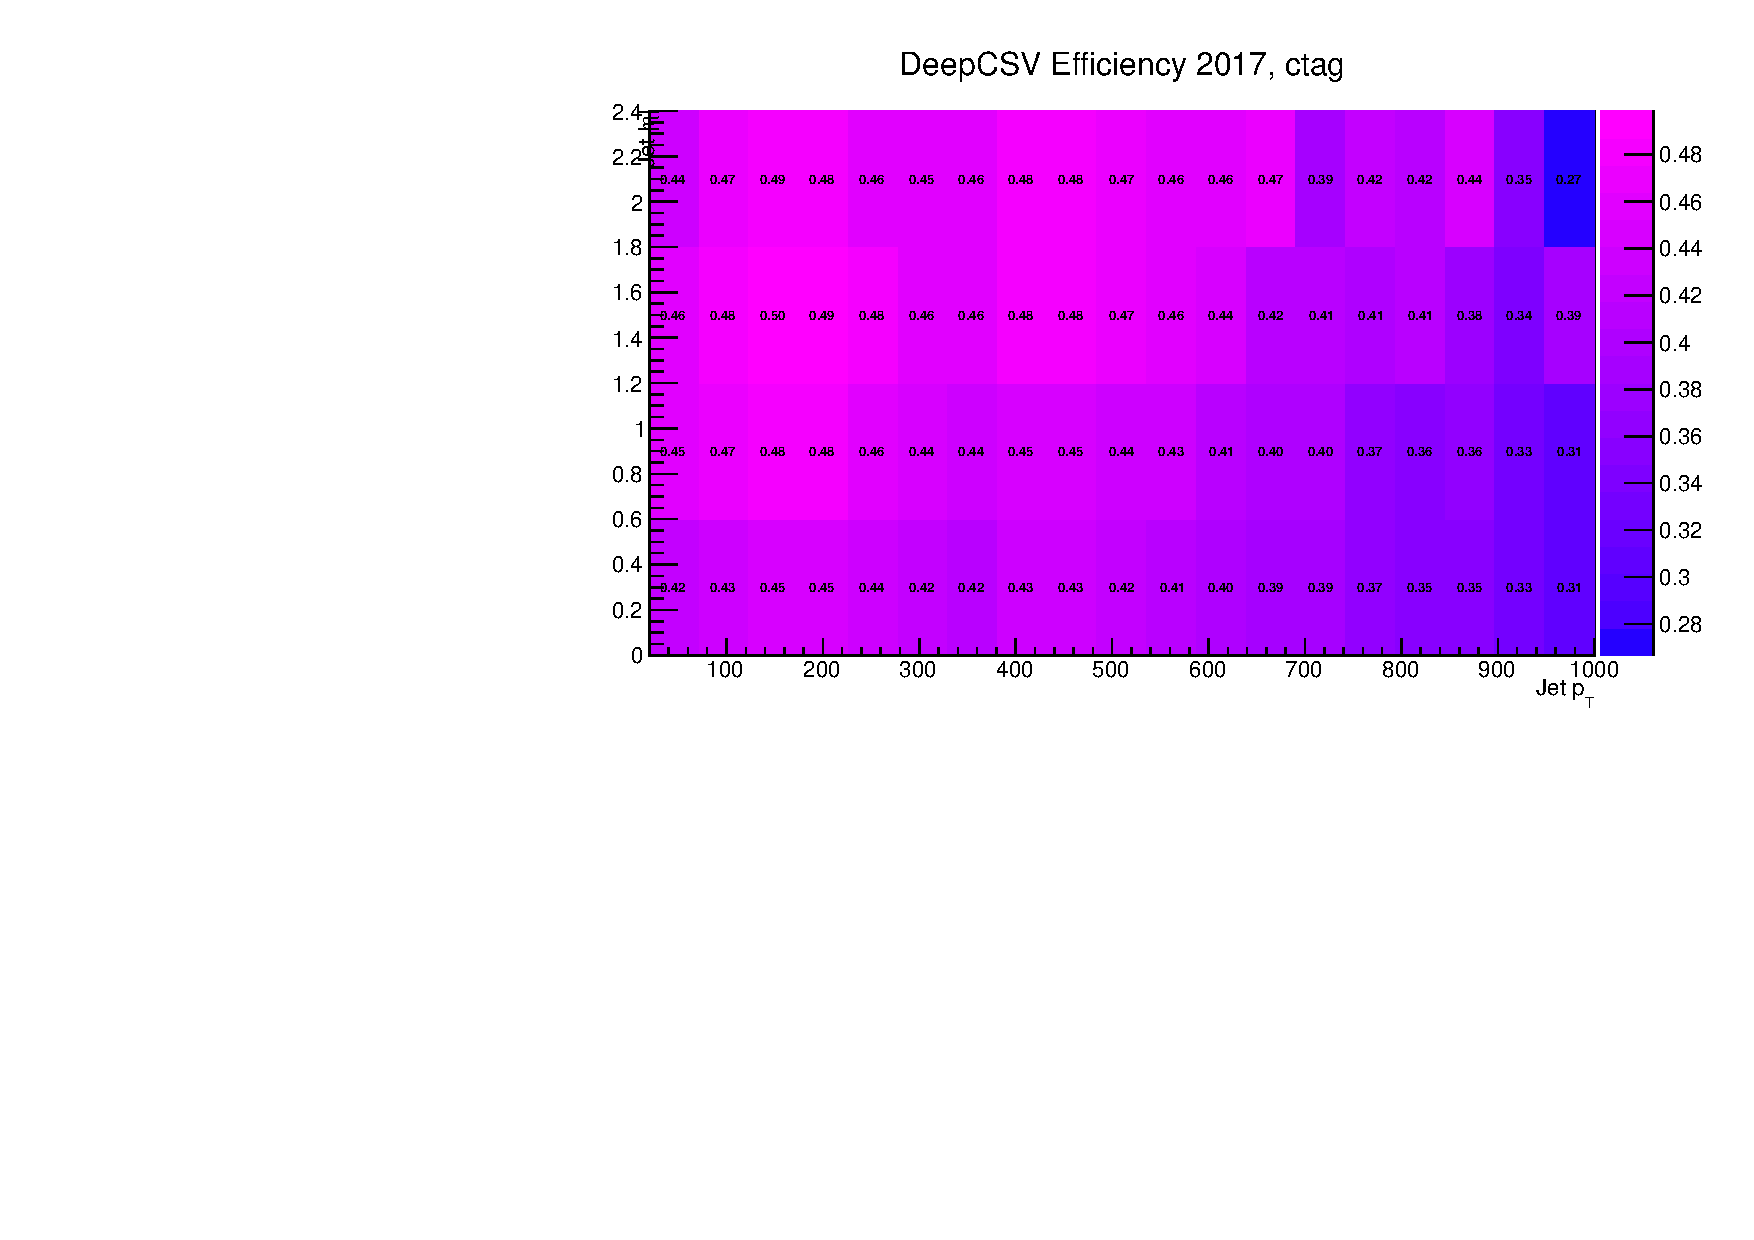
\includegraphics[width=0.5\textwidth]{Canvas_DeepCSV_SF_2017_ctag.pdf}
        \caption{Histogramme 2D des facteurs correctifs pour l'efficacité de l'étiquetage \Pcharm{} avec l'algorithme DeepCSV. L'abscisse est l'impulsion transverse \pt du jet considéré et l'ordonnée est sa pseudo-rapidité en valeur absolue $|\eta|$.}
    \end{center}
\end{figure}

\begin{figure}[H]
    \begin{center}
        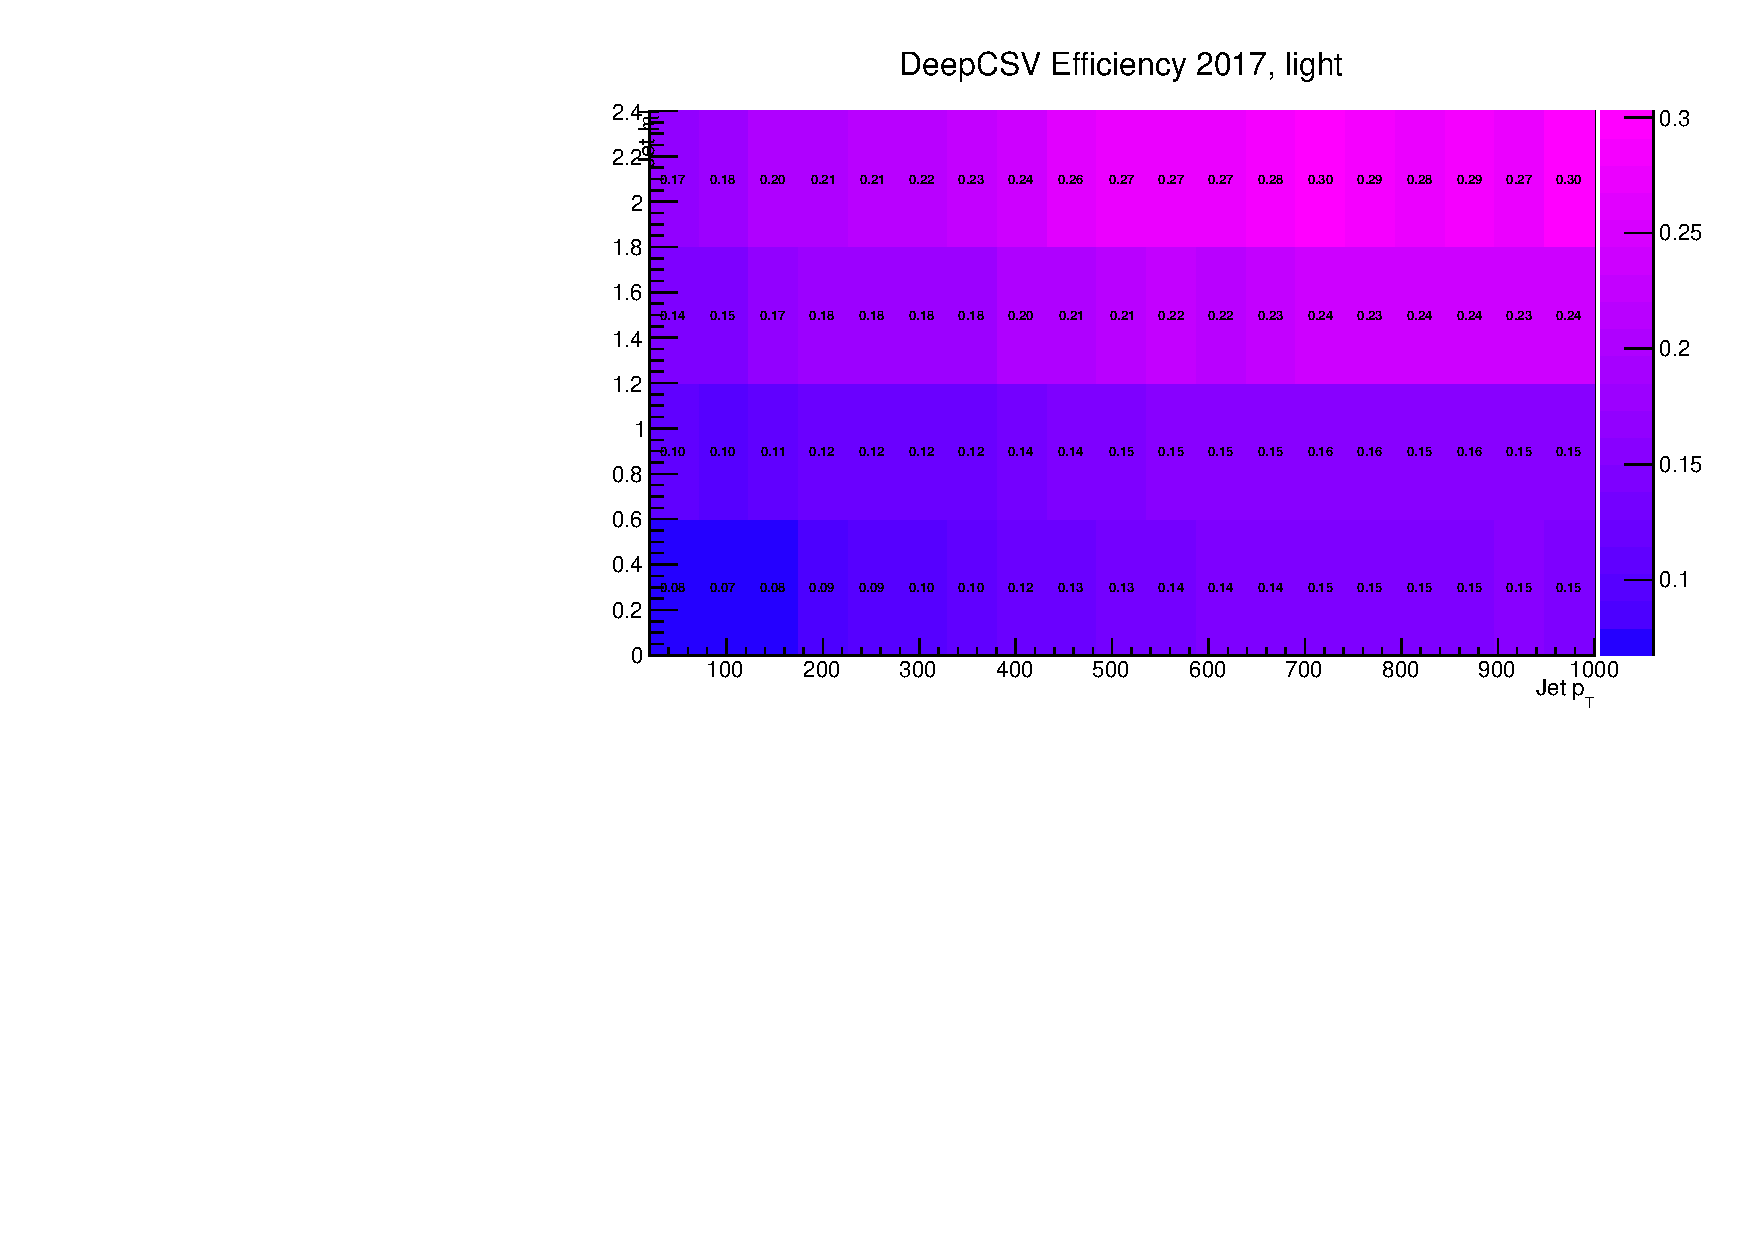
\includegraphics[width=0.5\textwidth]{Canvas_DeepCSV_SF_2017_light.pdf}
        \caption{Histogramme 2D des facteurs correctifs pour l'efficacité de l'étiquetage des lights jets avec l'algorithme DeepCSV. L'abscisse est l'impulsion transverse \pt du jet considéré et l'ordonnée est sa pseudo-rapidité en valeur absolue $|\eta|$.}
    \end{center}
\end{figure}



\section{Comparaison DATA/Monte-Carlo pré-fits}\label{comparaison}


\begin{figure}[H]
    \begin{subfigure}[b]{0.5\textwidth}
    \begin{center}
        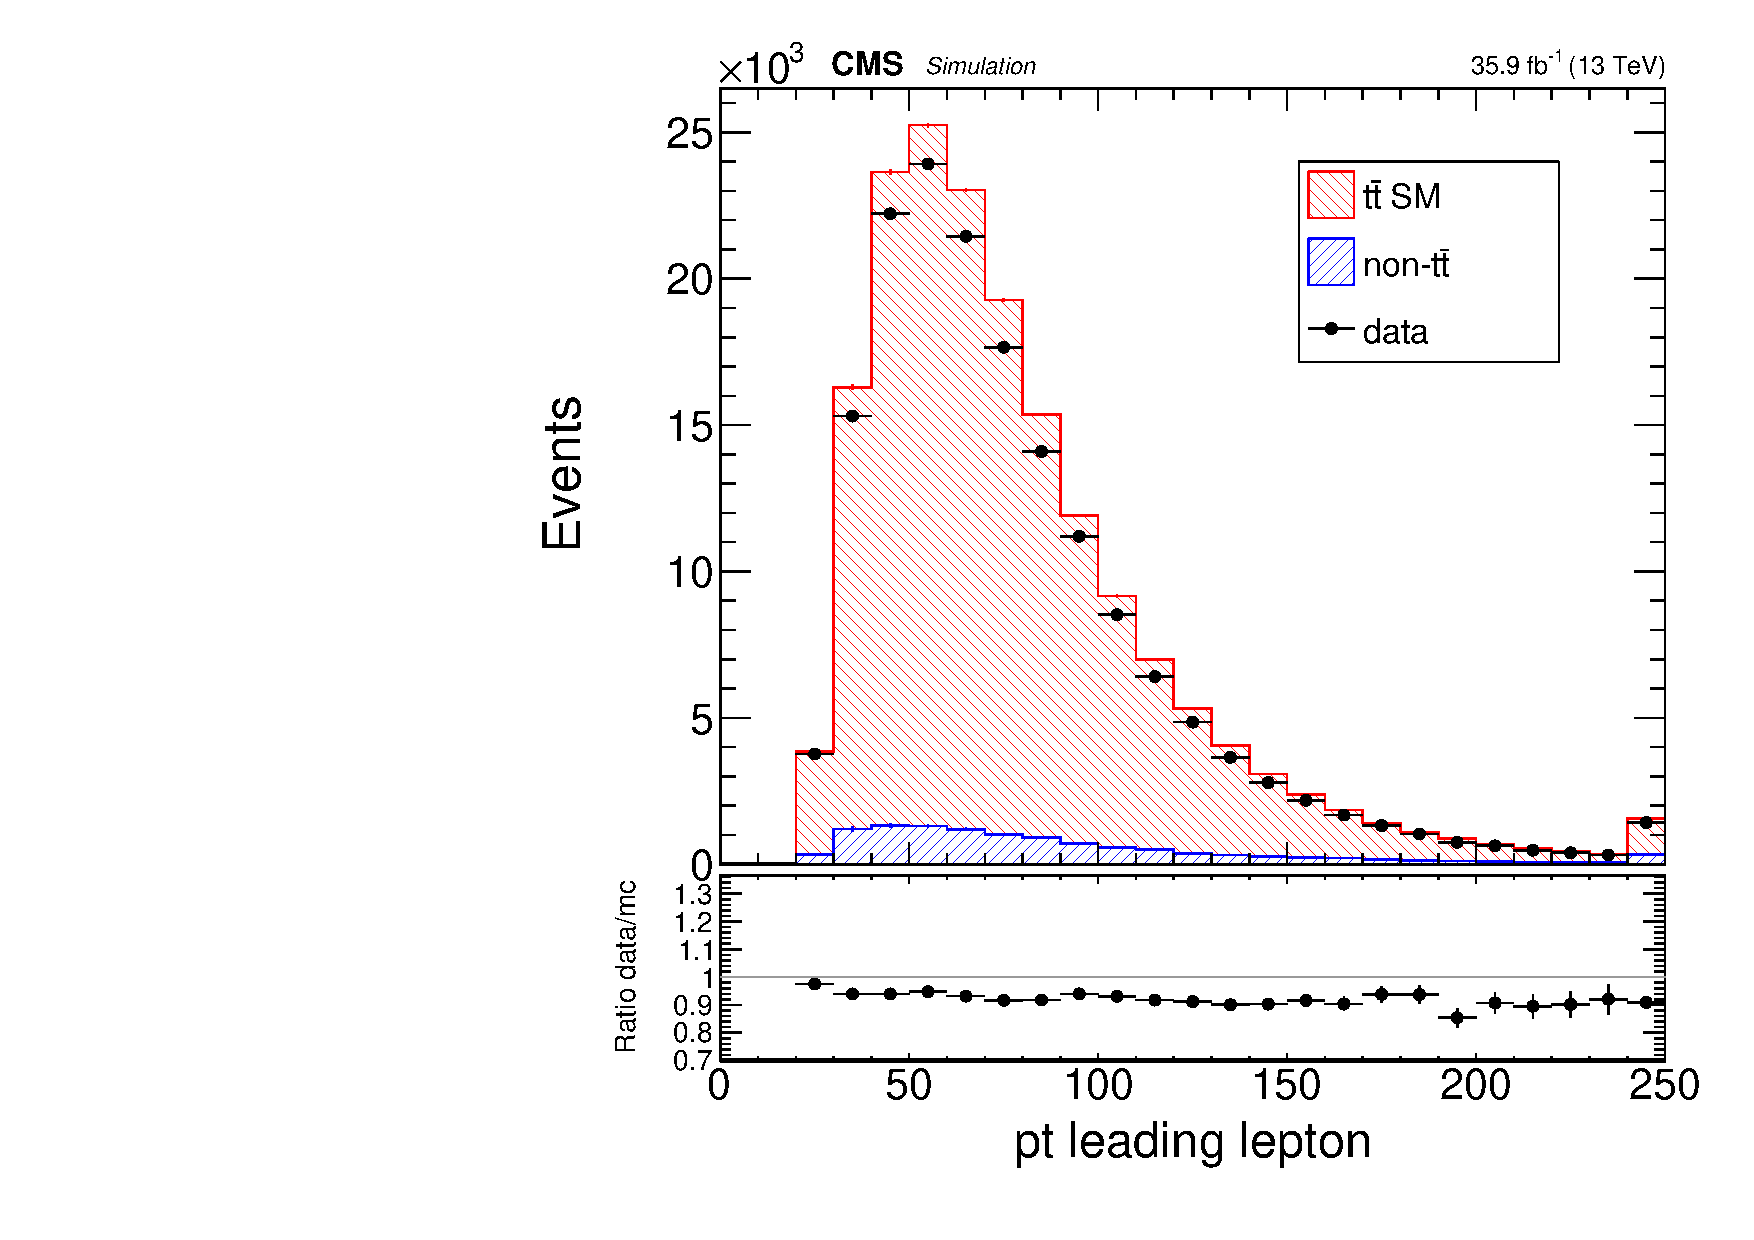
\includegraphics[width=0.8\textwidth, angle=-90]{pt_lead_2016.pdf}
        \caption{2016}
        \label{fig:nb_2016}
    \end{center}
    \end{subfigure}
    \begin{subfigure}[b]{0.5\textwidth}
    \begin{center}
        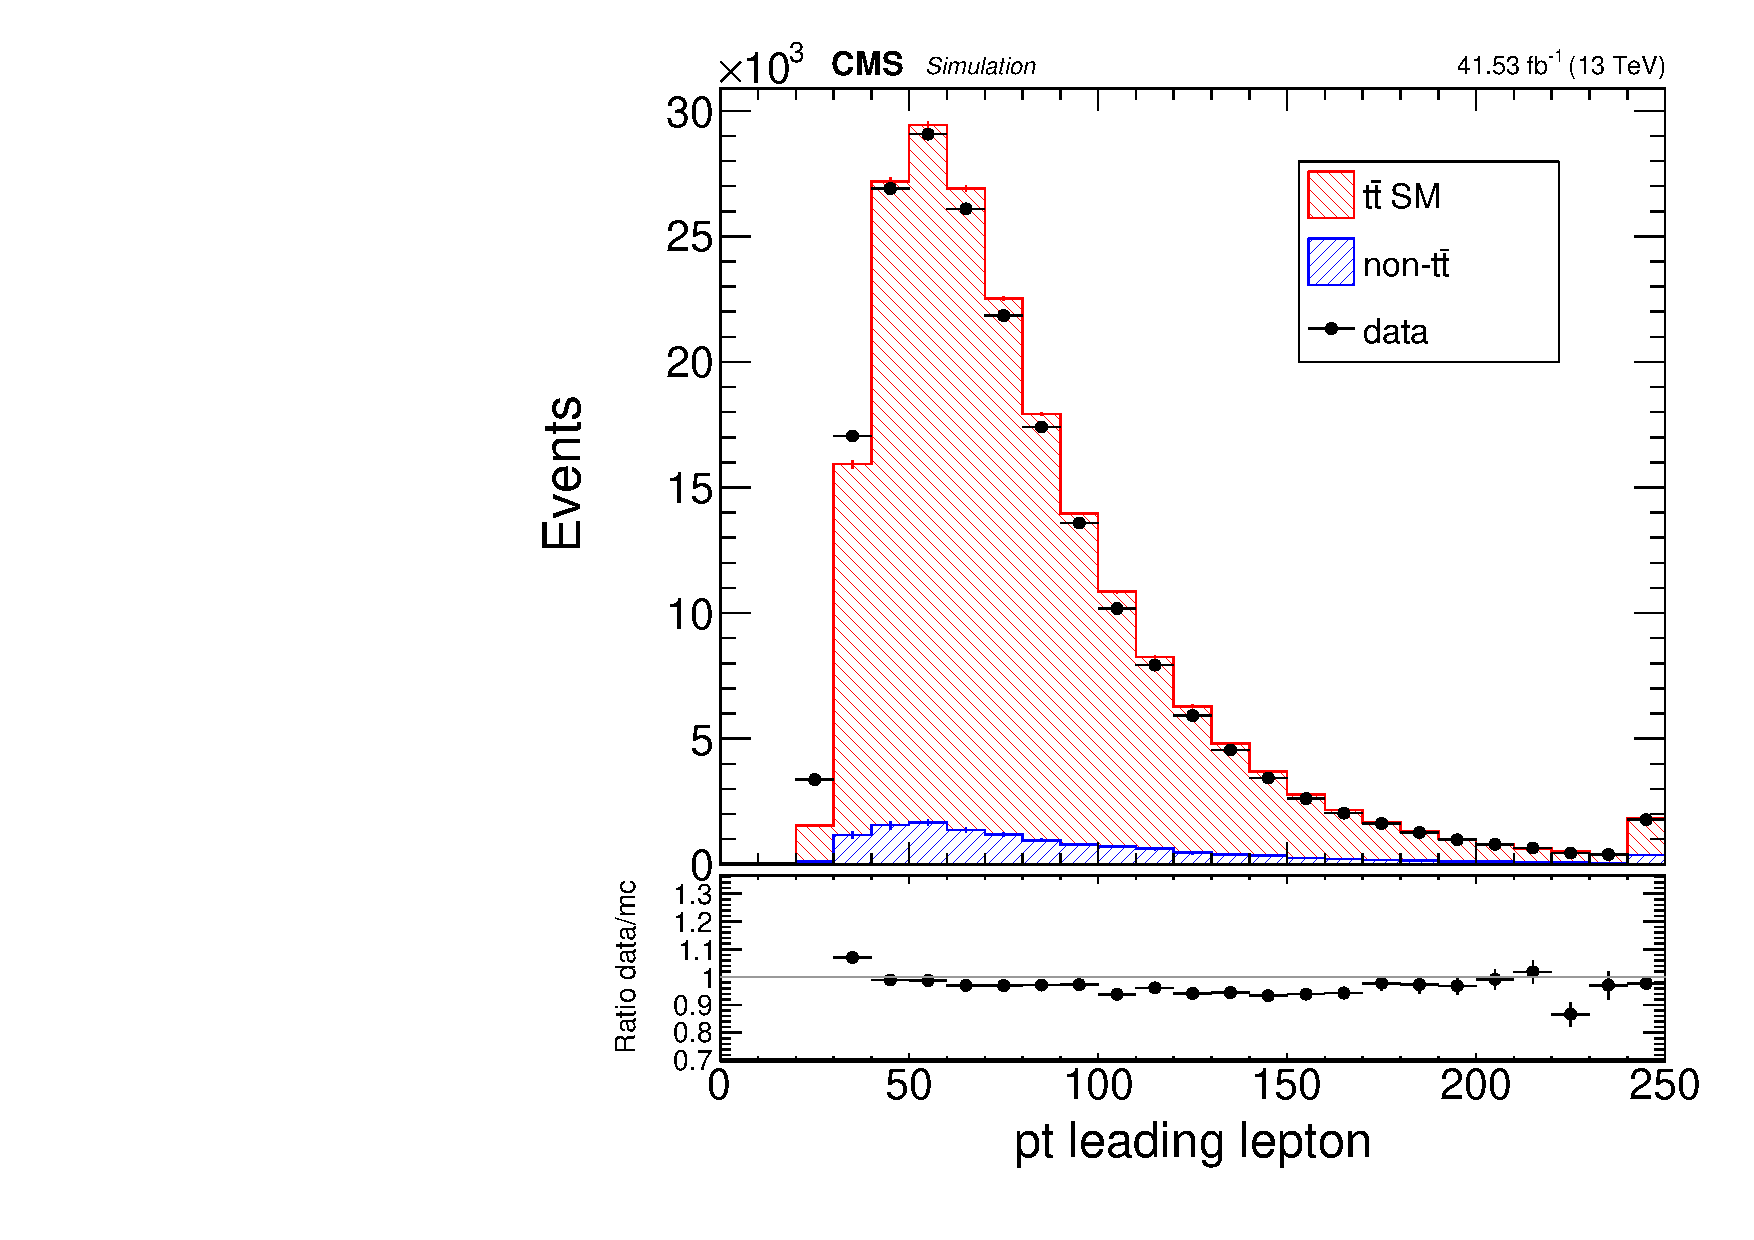
\includegraphics[width=0.8\textwidth, angle=-90]{pt_lead_2017.pdf}
        \caption{2017}
        \label{fig:nb_2017}
    \end{center}
    \end{subfigure}
    \caption{Comparaison données/Monte-Carlo pour le \pt du lepton leader pour l'année (\subref{fig:nb_2016}) 2016 et (\subref{fig:nb_2017}) 2017.}
\end{figure}

\begin{figure}[H]
    \begin{subfigure}[b]{0.5\textwidth}
    \begin{center}
        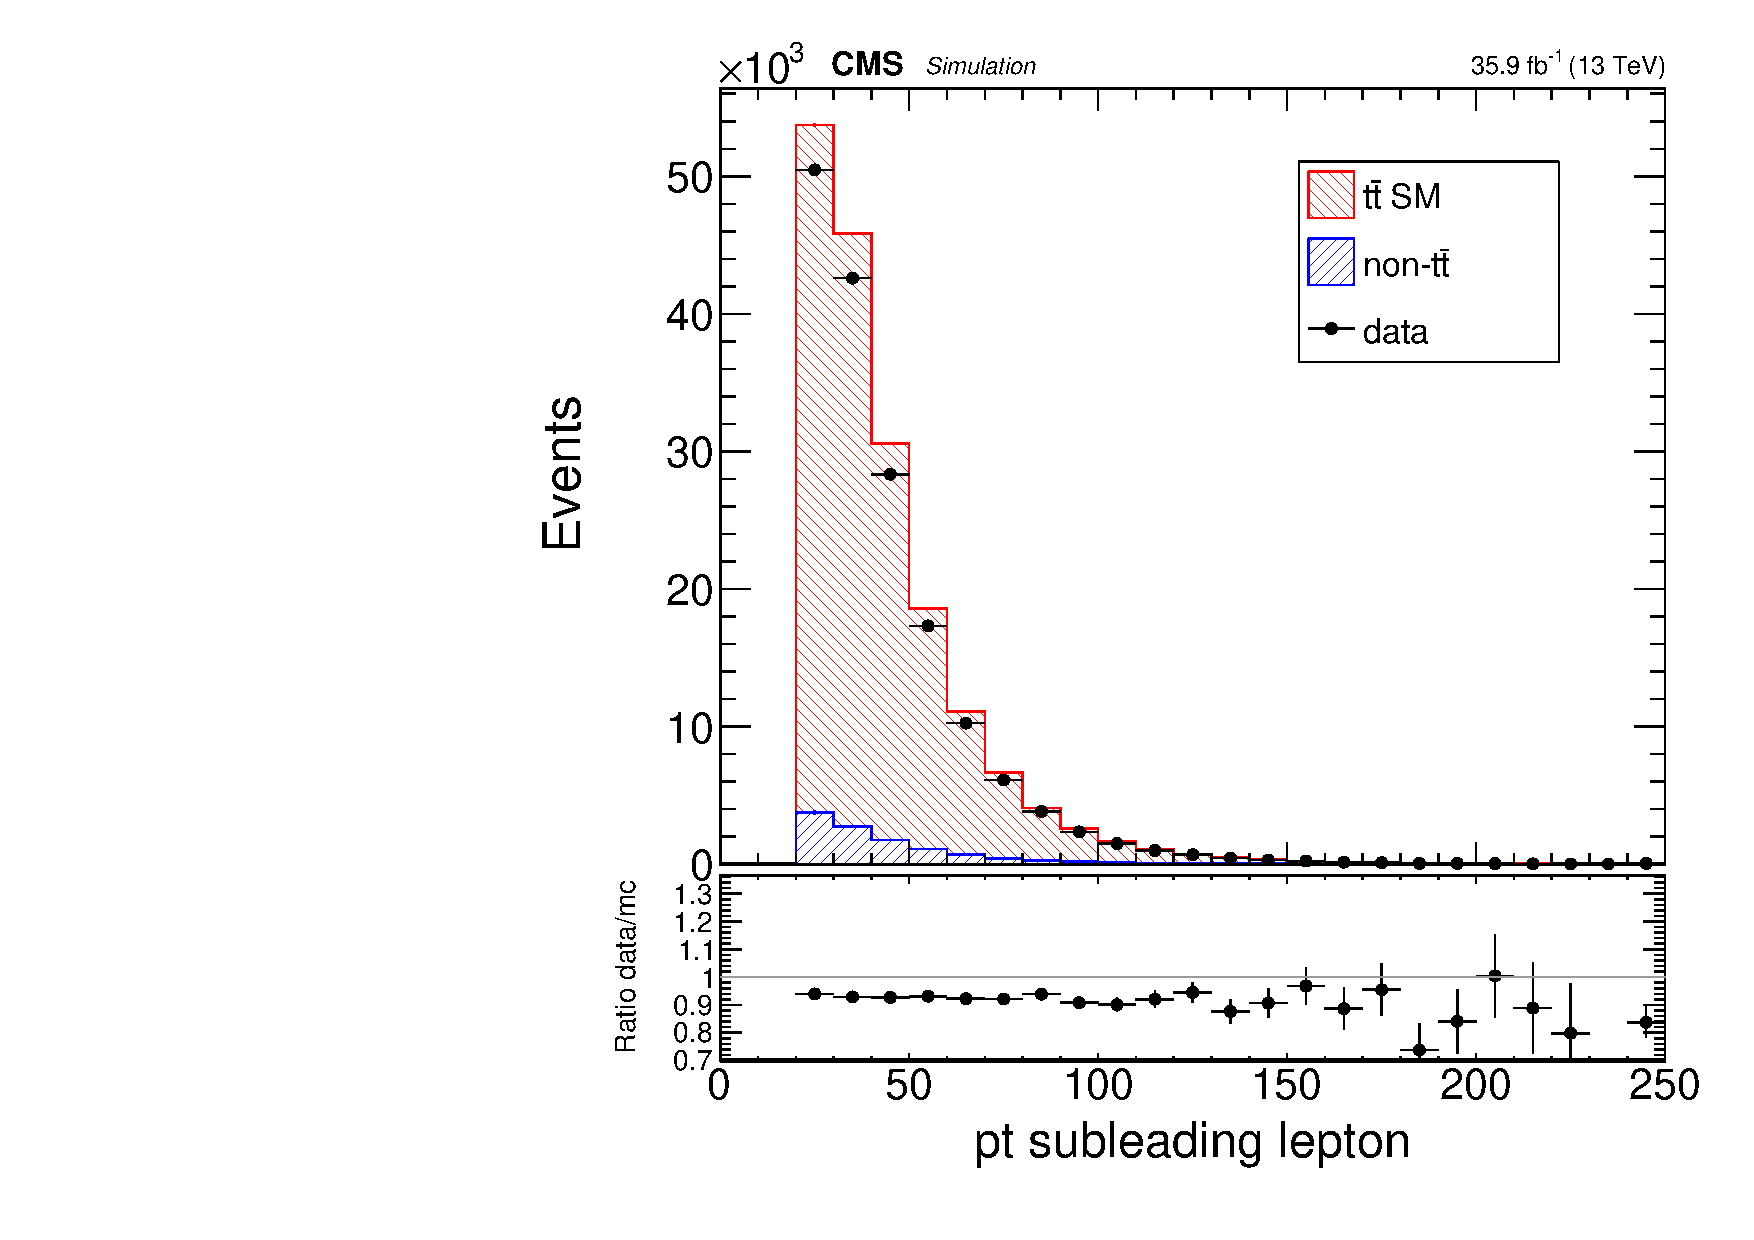
\includegraphics[width=0.8\textwidth, angle=-90]{pt_sublead_2016.pdf}
        \caption{2016}
        \label{fig:nb_2016}
    \end{center}
    \end{subfigure}
    \begin{subfigure}[b]{0.5\textwidth}
    \begin{center}
        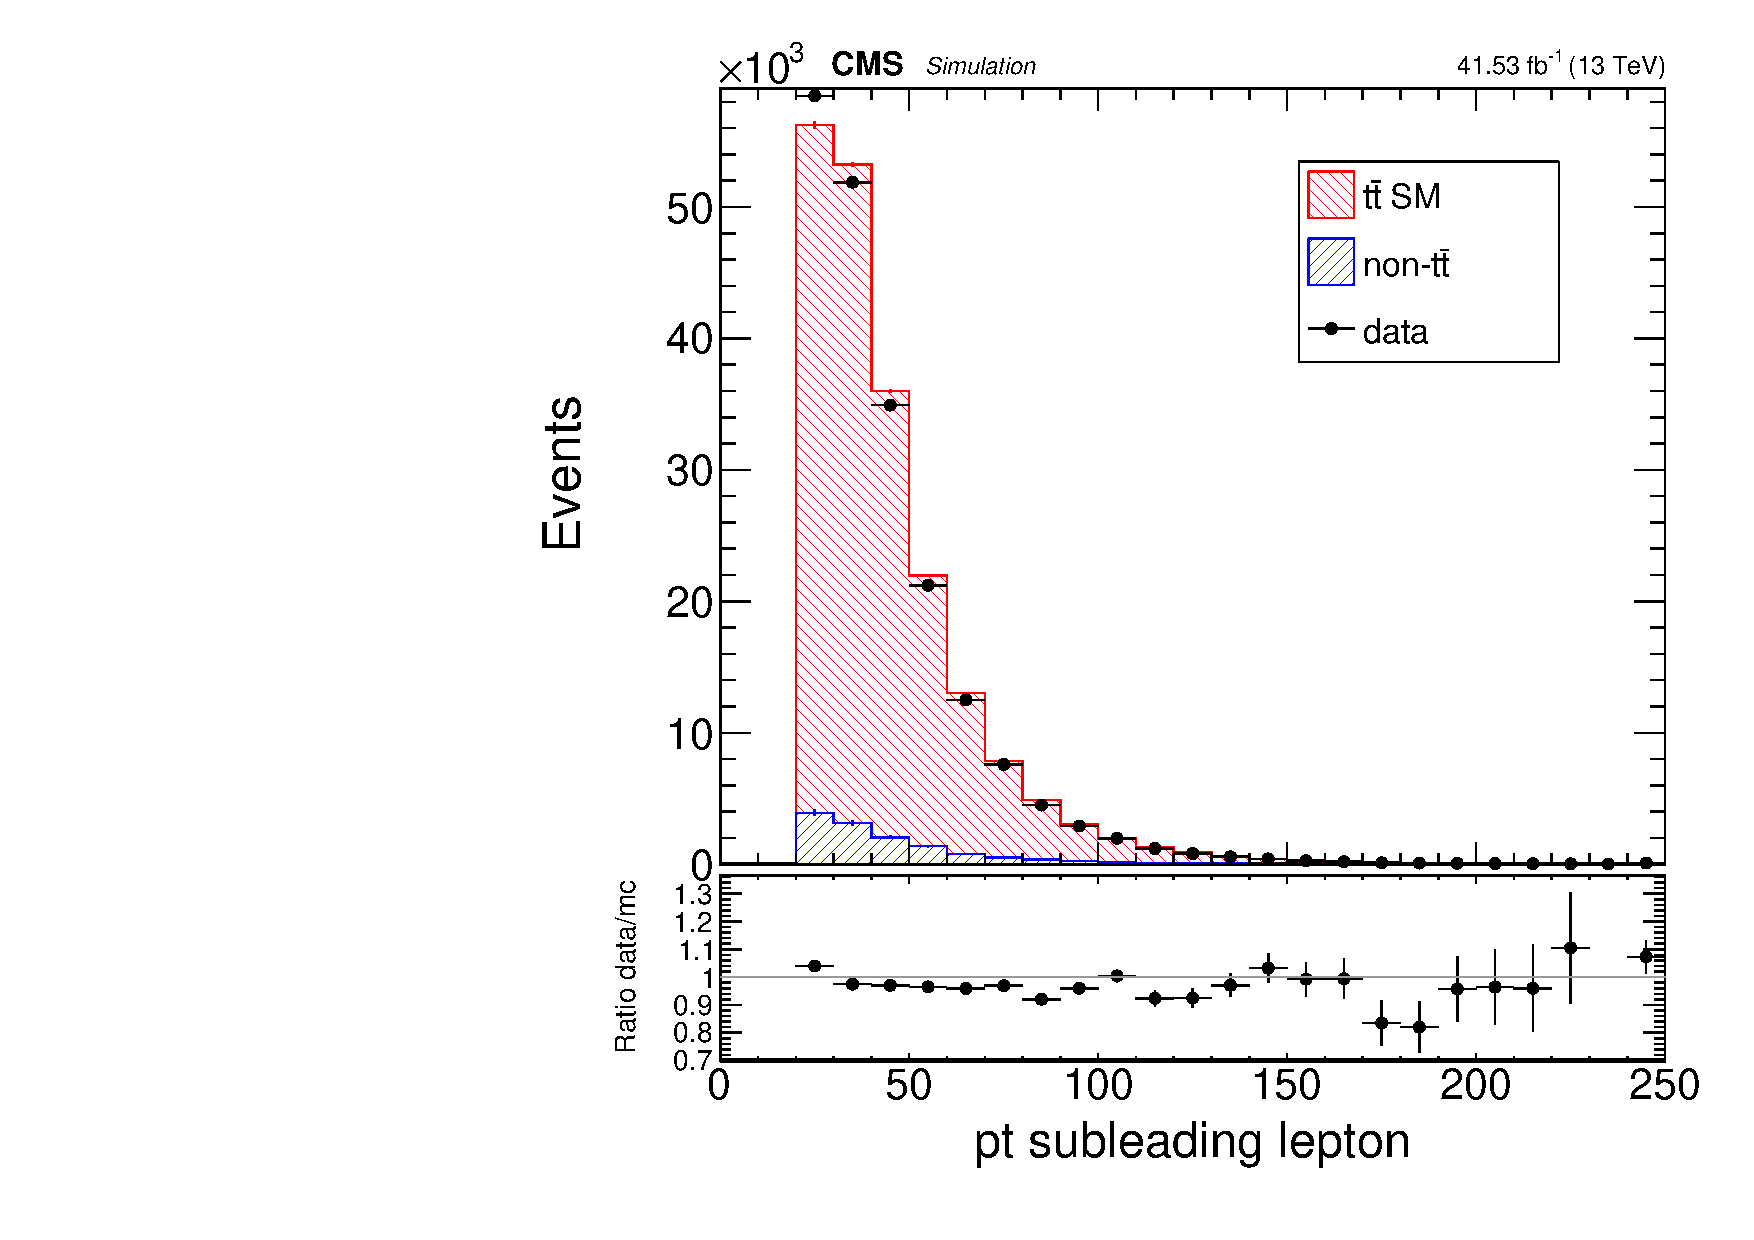
\includegraphics[width=0.8\textwidth, angle=-90]{pt_sublead_2017.pdf}
        \caption{2017}
        \label{fig:nb_2017}
    \end{center}
    \end{subfigure}
    \caption{Comparaison données/Monte-Carlo pour le \pt du lepton subleader pour l'année (\subref{fig:nb_2016}) 2016 et (\subref{fig:nb_2017}) 2017.}
\end{figure}


\begin{figure}[H]
    \begin{subfigure}[b]{0.5\textwidth}
    \begin{center}
        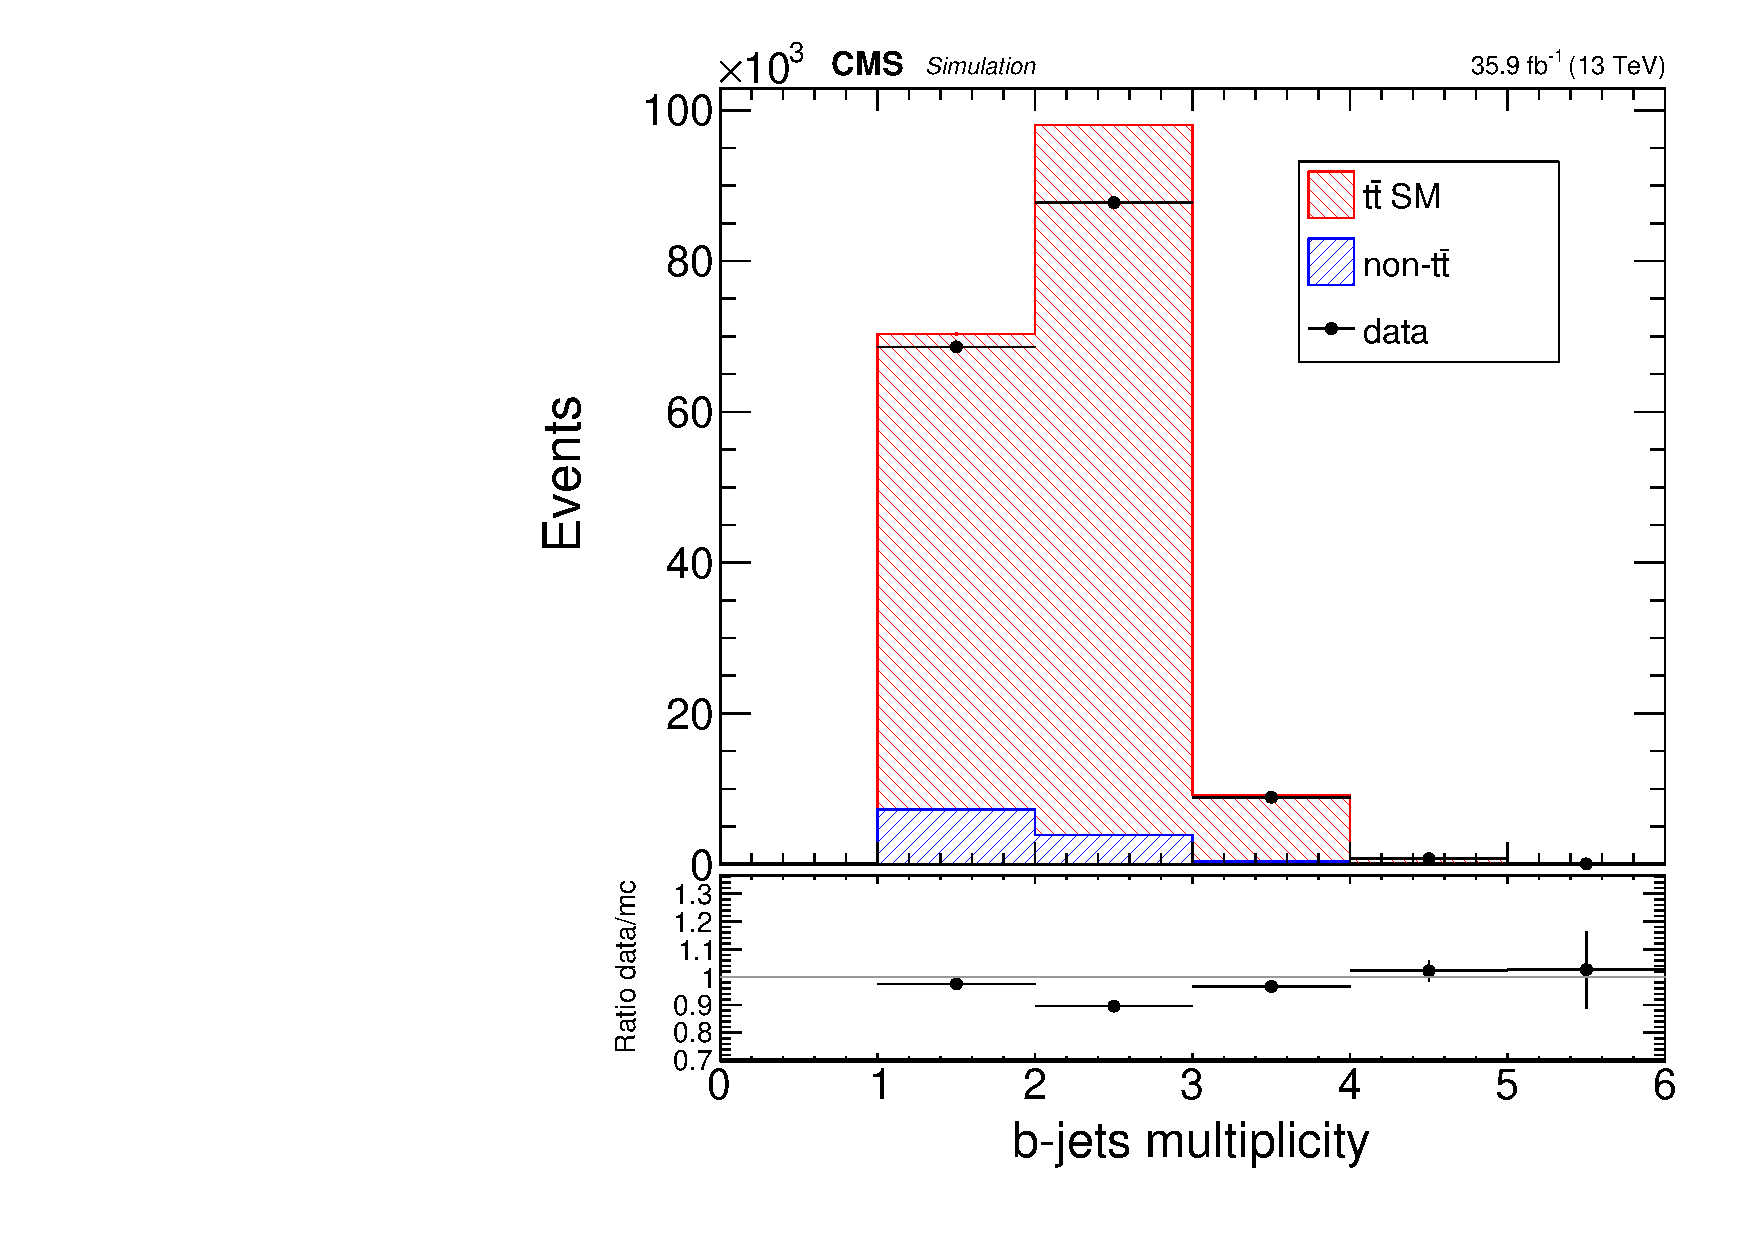
\includegraphics[width=0.8\textwidth, angle=-90]{n_bjets_2016.pdf}
        \caption{2016}
        \label{fig:nb_2016}
    \end{center}
    \end{subfigure}
    \begin{subfigure}[b]{0.5\textwidth}
    \begin{center}
        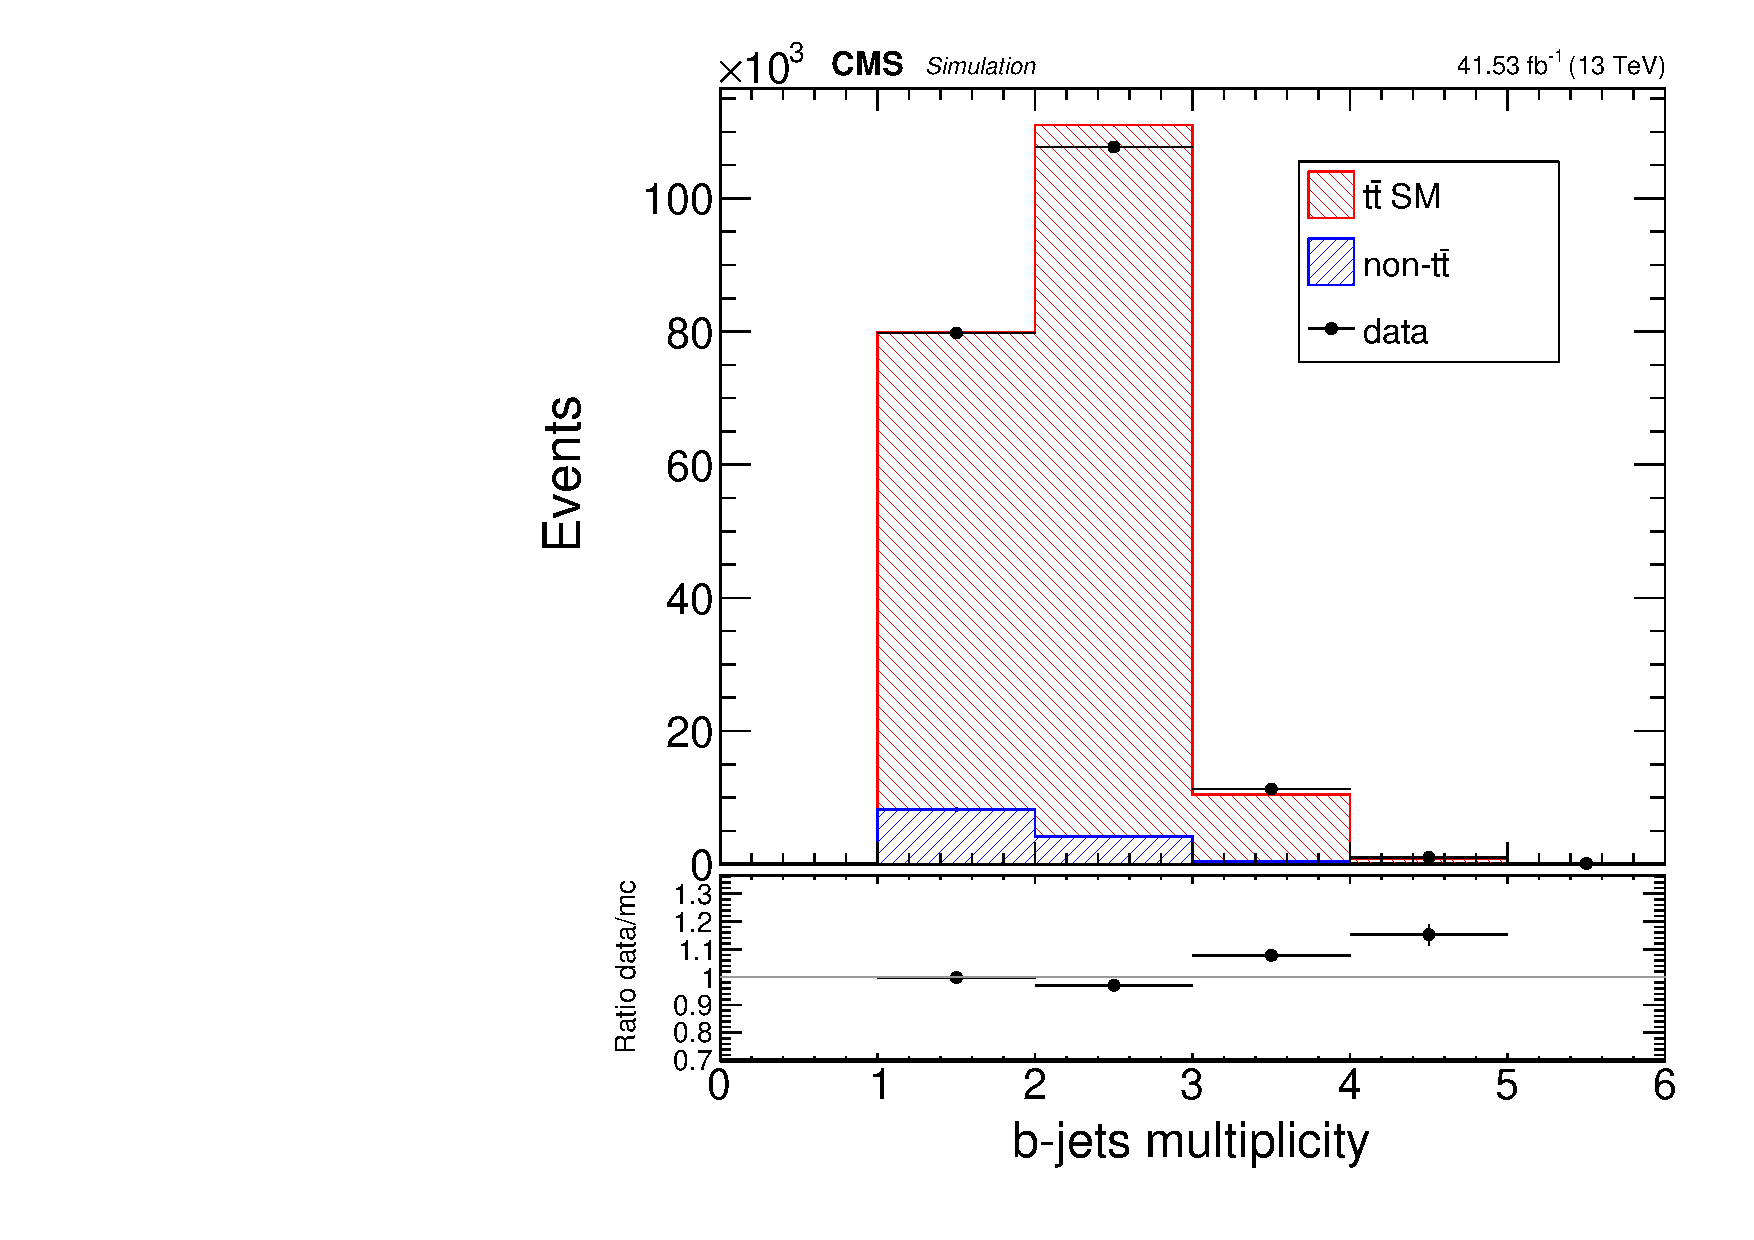
\includegraphics[width=0.8\textwidth, angle=-90]{n_bjets_2017.pdf}
        \caption{2017}
        \label{fig:nb_2017}
    \end{center}
    \end{subfigure}
    \caption{Comparaison données/Monte-Carlo pour le nombre de jets étiqueté $\Pbottom$ pour l'année (\subref{fig:nb_2016}) 2016 et (\subref{fig:nb_2017}) 2017.}
\end{figure}

\begin{figure}[H]
    \begin{subfigure}[b]{0.5\textwidth}
    \begin{center}
        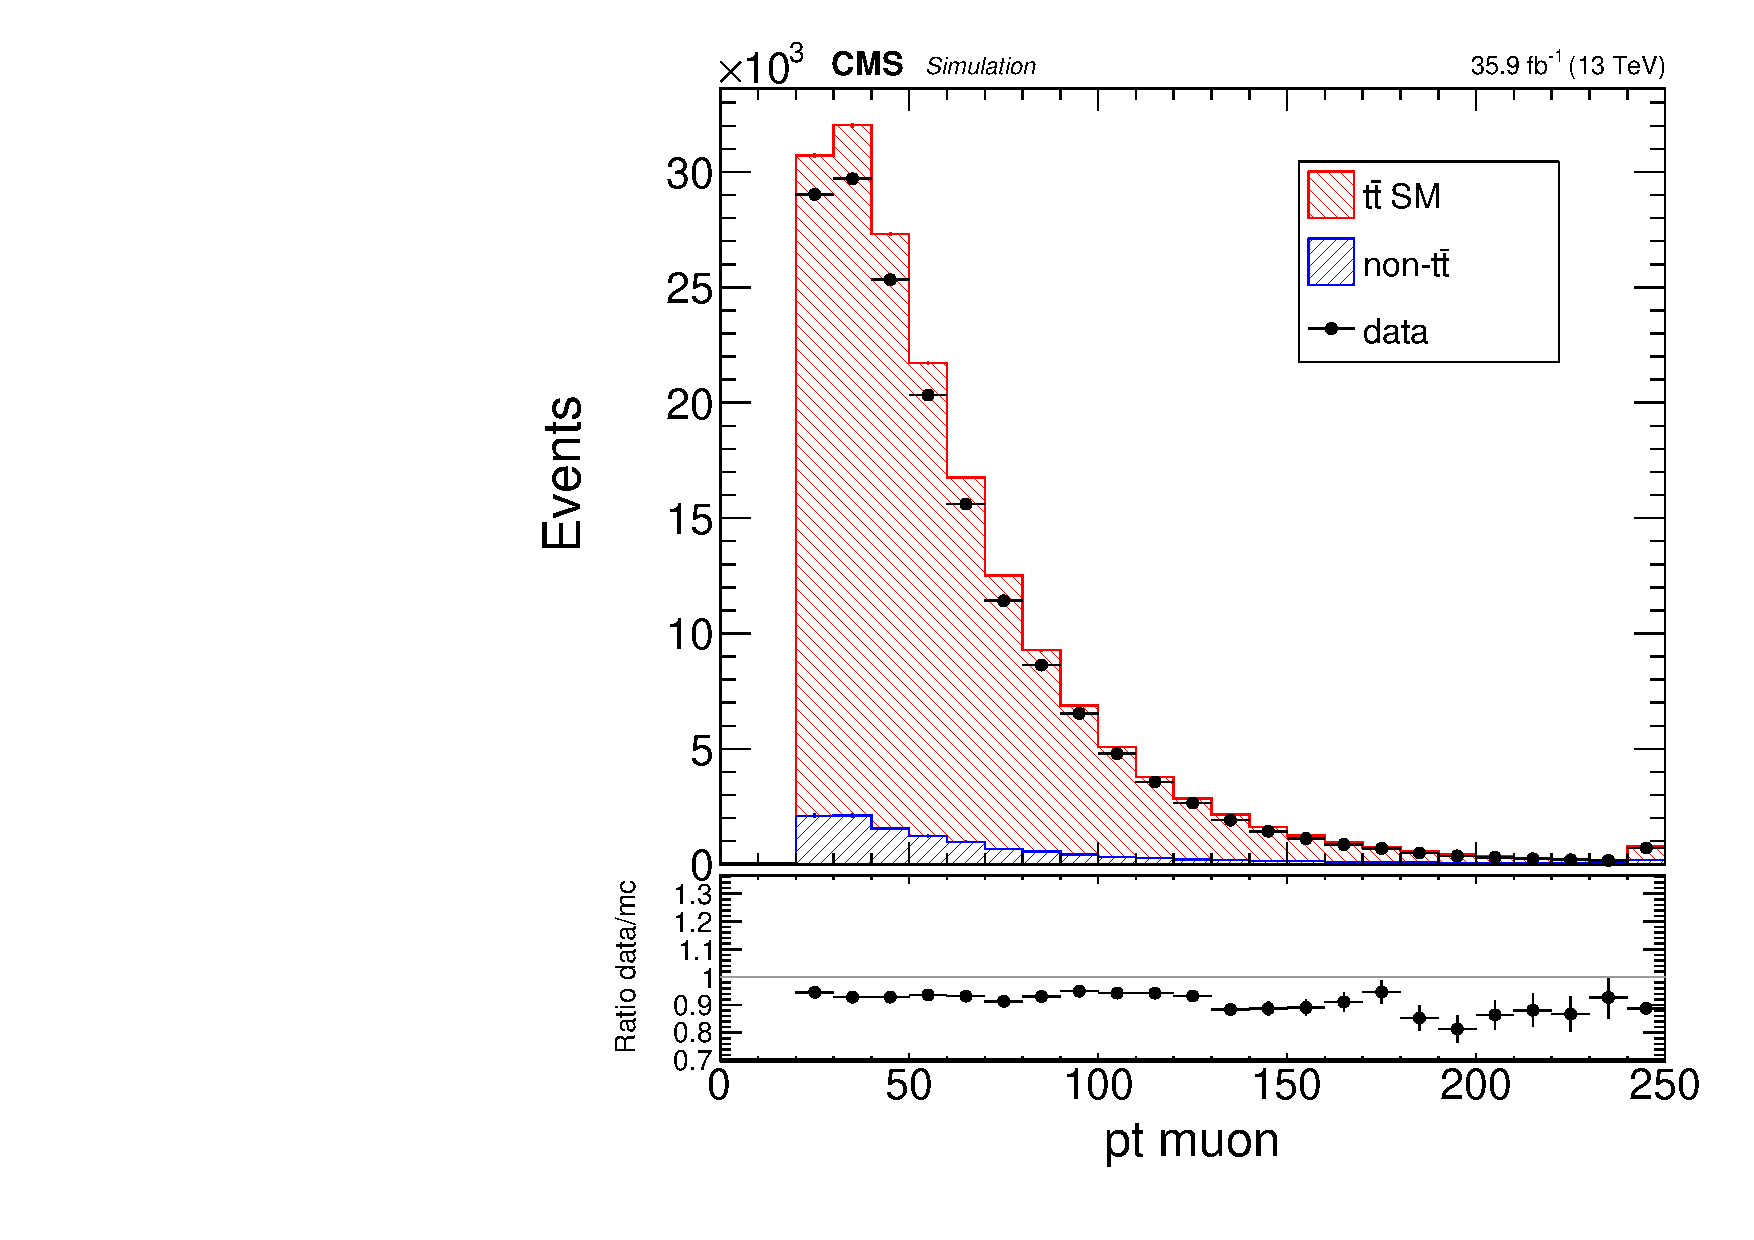
\includegraphics[width=0.8\textwidth, angle=-90]{pt_muon_2016.pdf}
        \caption{2016}
        \label{fig:nb_2016}
    \end{center}
    \end{subfigure}
    \begin{subfigure}[b]{0.5\textwidth}
    \begin{center}
        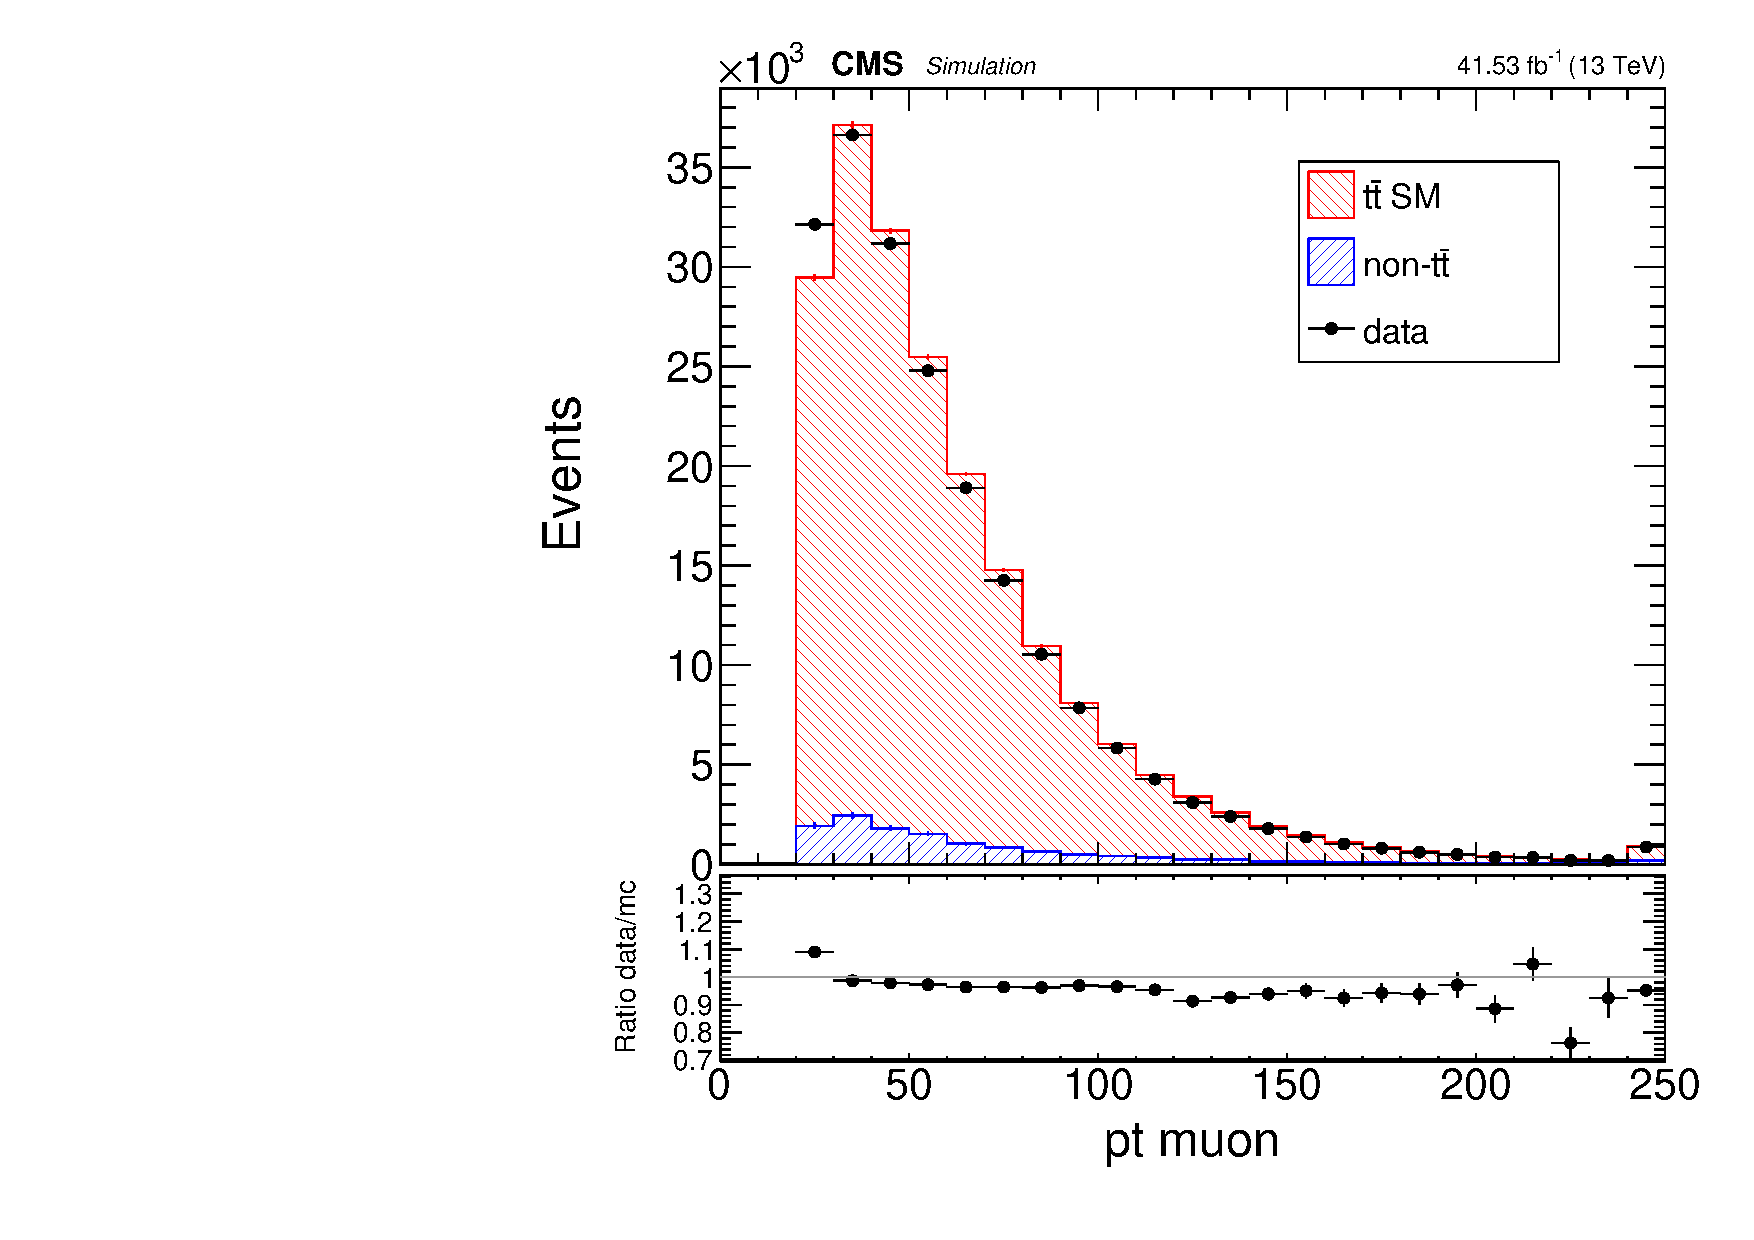
\includegraphics[width=0.8\textwidth, angle=-90]{pt_muon_2017.pdf}
        \caption{2017}
        \label{fig:nb_2017}
    \end{center}
    \end{subfigure}
    \caption{Comparaison données/Monte-Carlo pour le \pt du muon pour l'année (\subref{fig:nb_2016}) 2016 et (\subref{fig:nb_2017}) 2017.}
\end{figure}

\begin{figure}[H]
    \begin{subfigure}[b]{0.5\textwidth}
    \begin{center}
        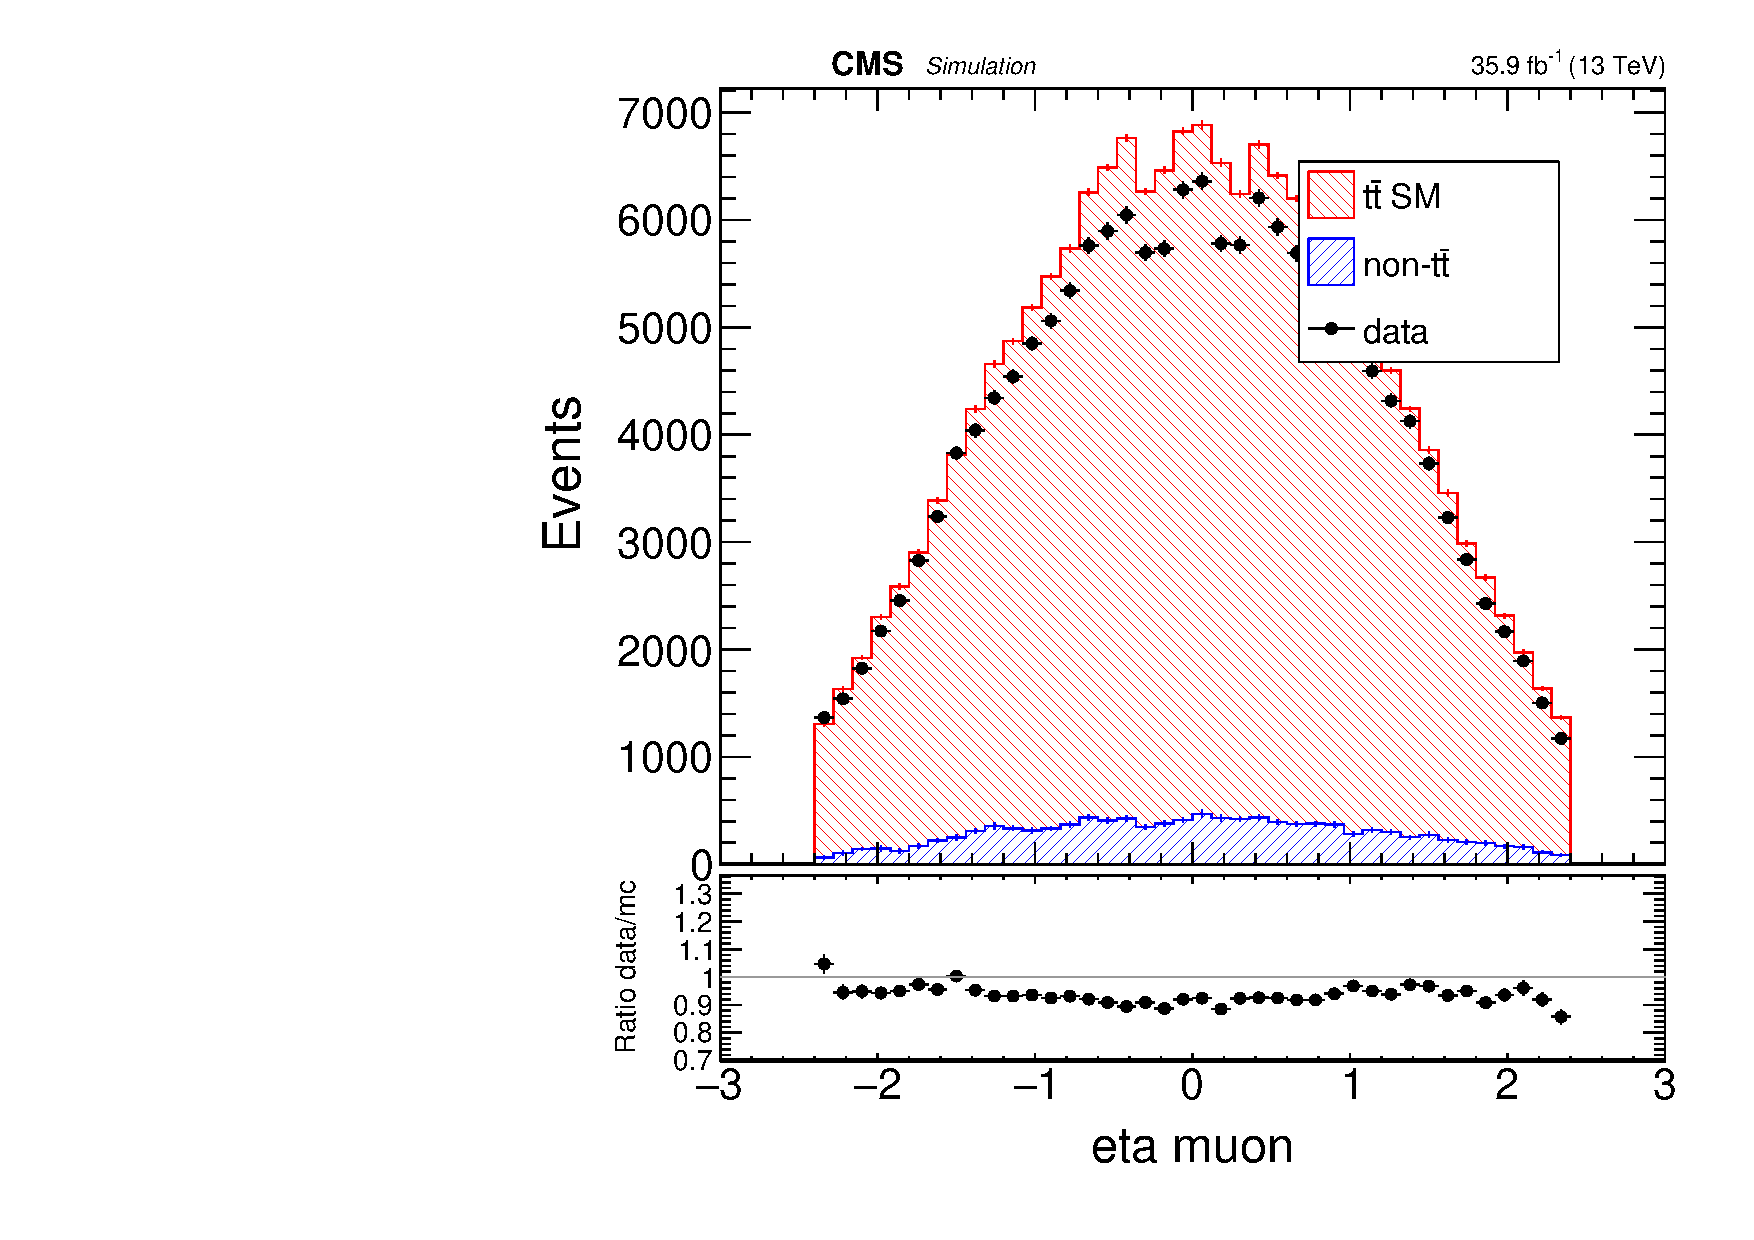
\includegraphics[width=0.8\textwidth, angle=-90]{eta_muon_2016.pdf}
        \caption{2016}
        \label{fig:nb_2016}
    \end{center}
    \end{subfigure}
    \begin{subfigure}[b]{0.5\textwidth}
    \begin{center}
        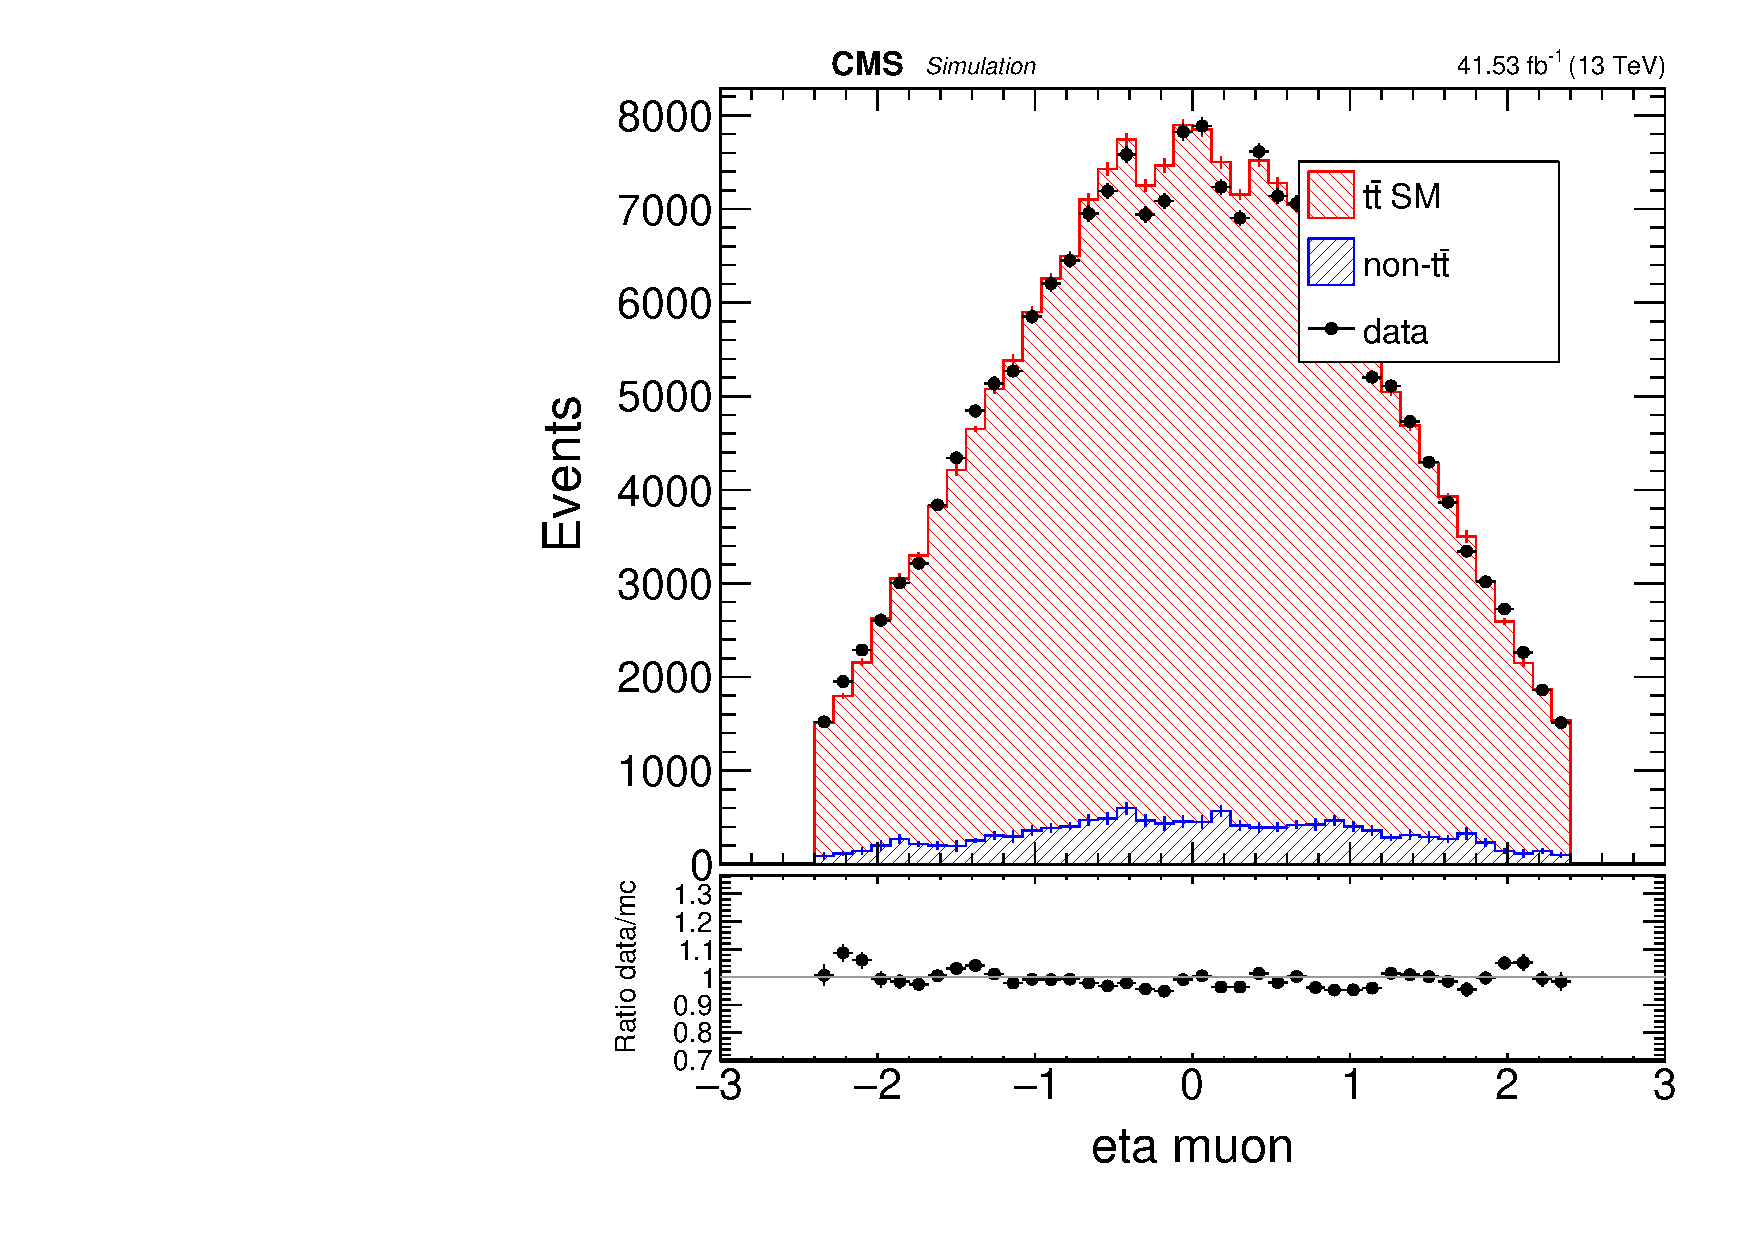
\includegraphics[width=0.8\textwidth, angle=-90]{eta_muon_2017.pdf}
        \caption{2017}
        \label{fig:nb_2017}
    \end{center}
    \end{subfigure}
    \caption{Comparaison données/Monte-Carlo pour le $\eta$ du muon pour l'année (\subref{fig:nb_2016}) 2016 et (\subref{fig:nb_2017}) 2017.}
\end{figure}

\begin{figure}[H]
    \begin{subfigure}[b]{0.5\textwidth}
    \begin{center}
        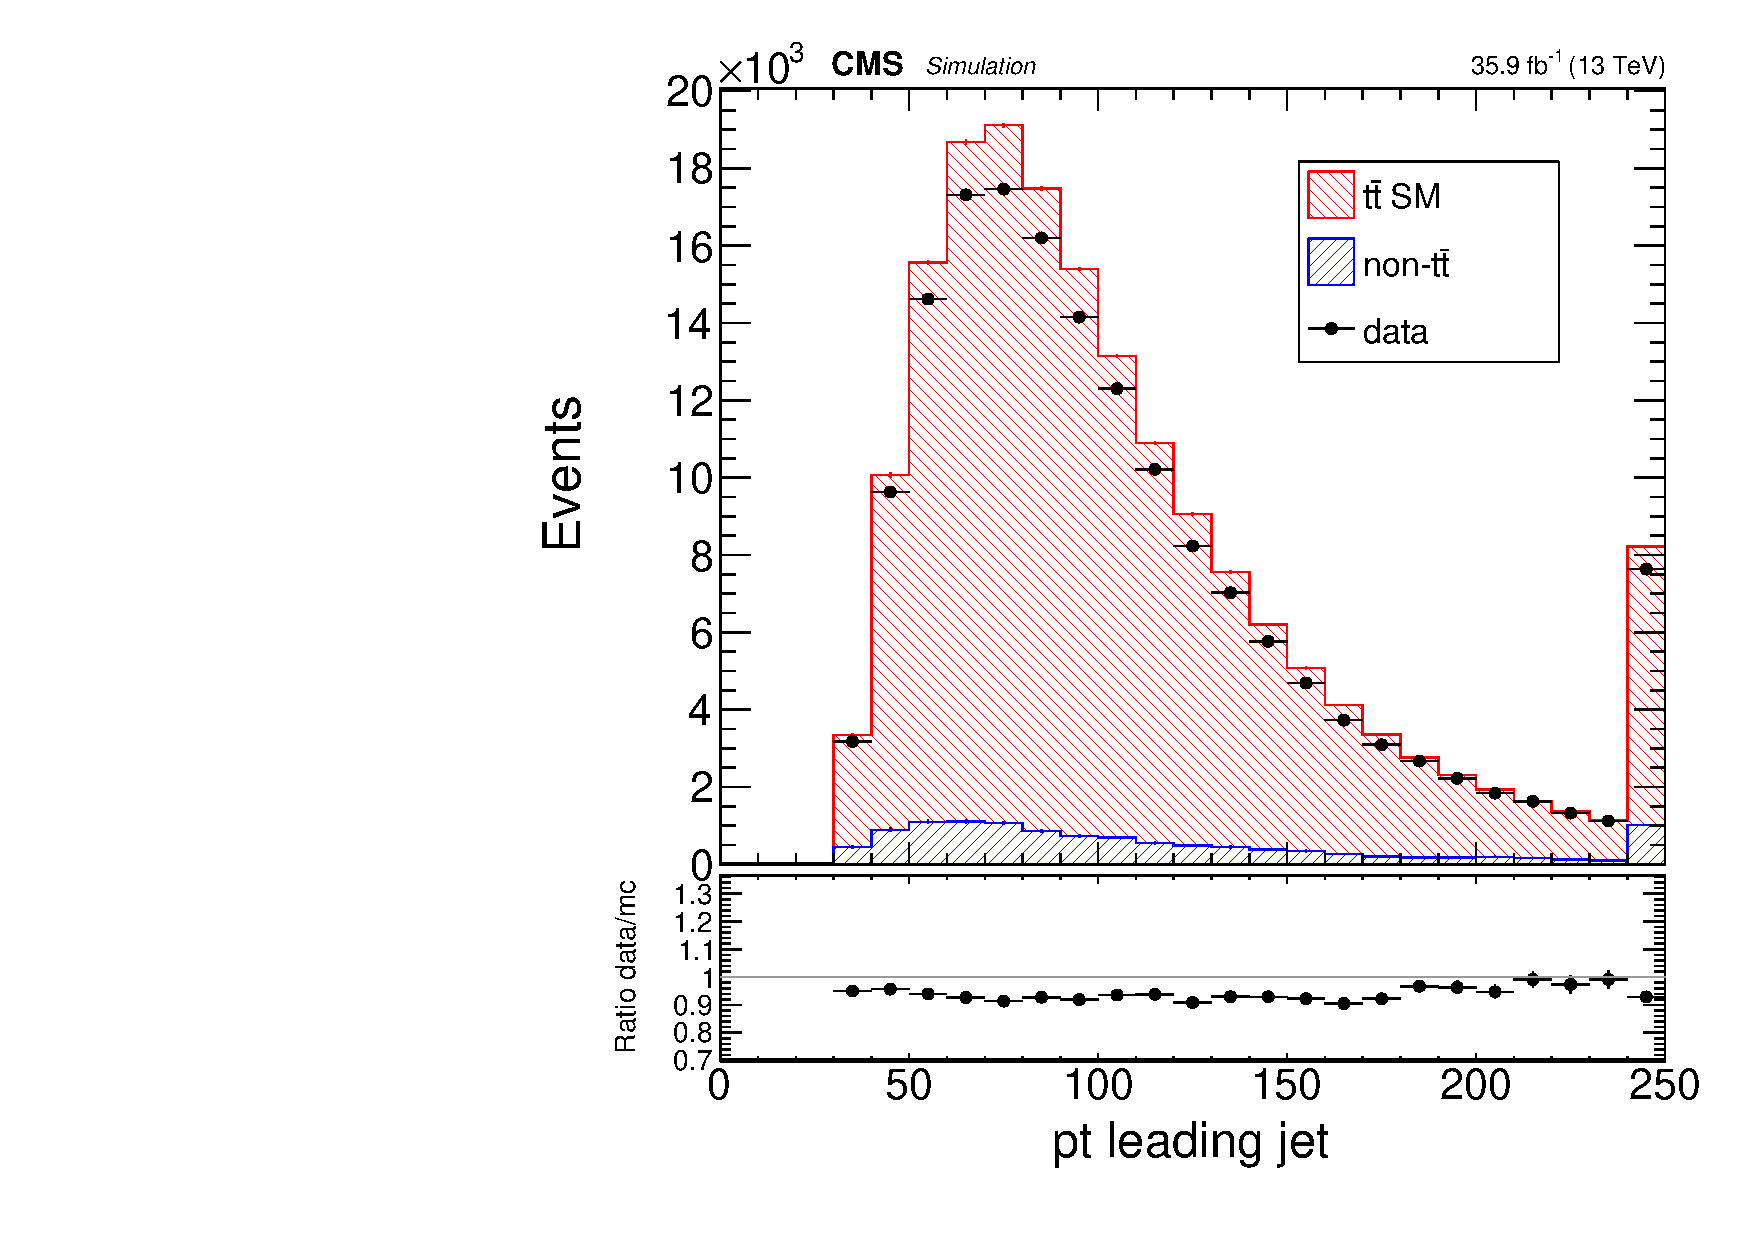
\includegraphics[width=0.8\textwidth, angle=-90]{j1_pt_2016.pdf}
        \caption{2016}
        \label{fig:nb_2016}
    \end{center}
    \end{subfigure}
    \begin{subfigure}[b]{0.5\textwidth}
    \begin{center}
        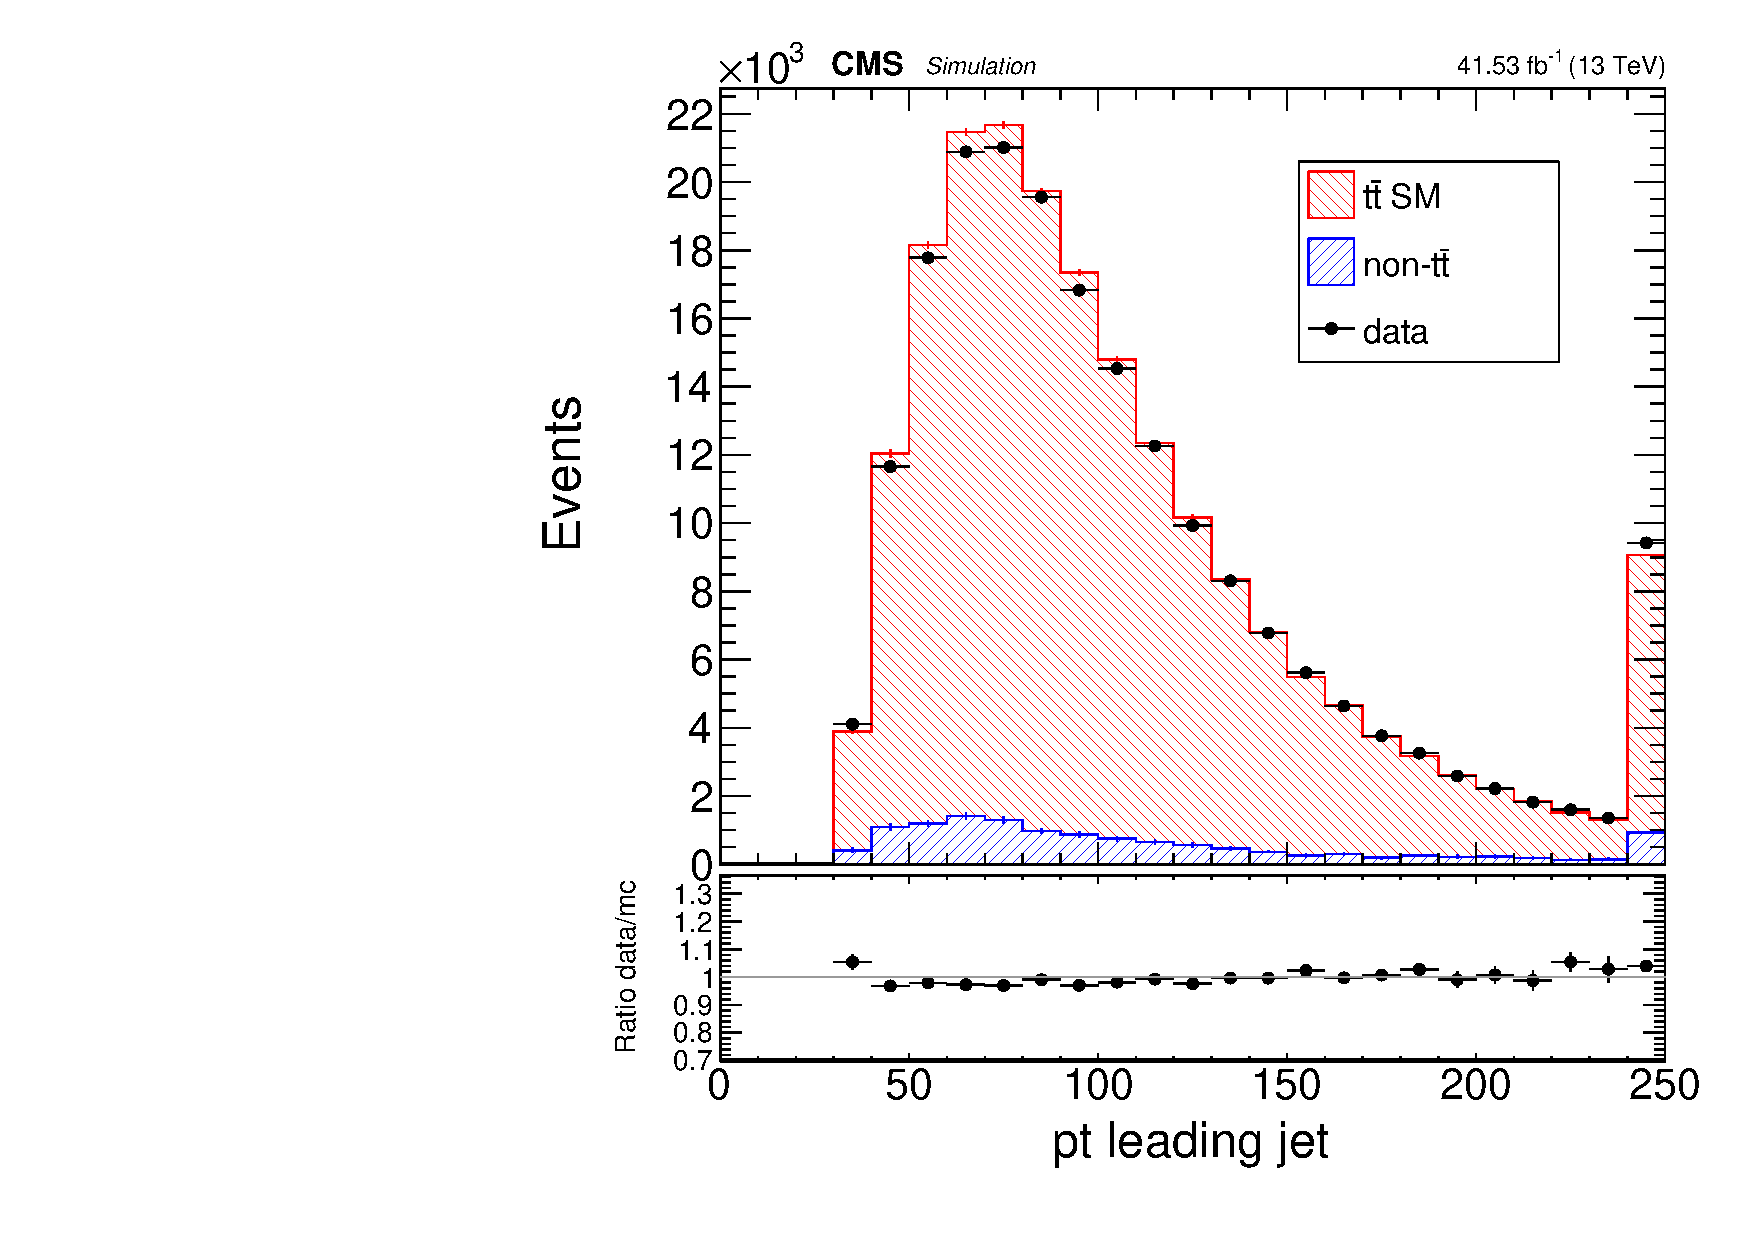
\includegraphics[width=0.8\textwidth, angle=-90]{j1_pt_2017.pdf}
        \caption{2017}
        \label{fig:nb_2017}
    \end{center}
    \end{subfigure}
    \caption{Comparaison données/Monte-Carlo pour le \pt du jet leader pour l'année (\subref{fig:nb_2016}) 2016 et (\subref{fig:nb_2017}) 2017.}
\end{figure}

\begin{figure}[H]
    \begin{subfigure}[b]{0.5\textwidth}
    \begin{center}
        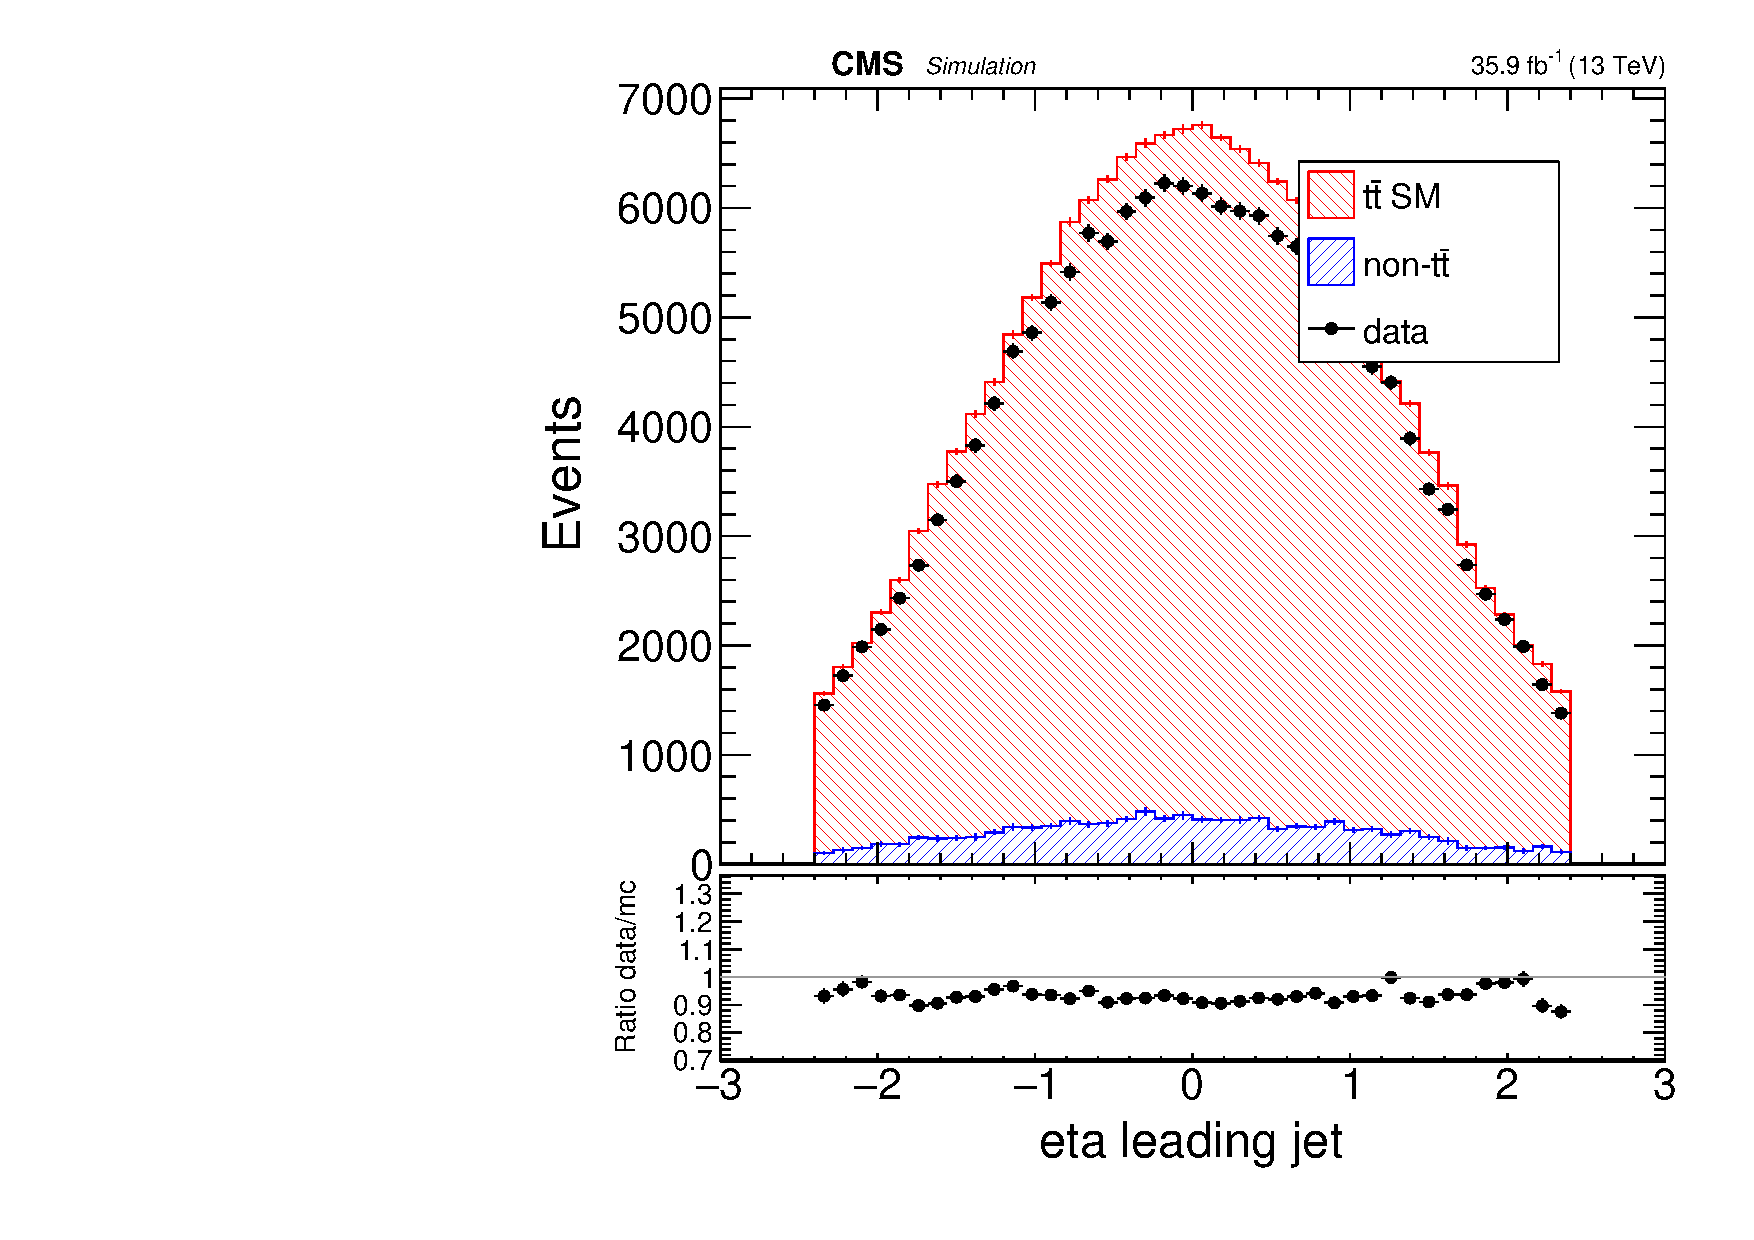
\includegraphics[width=0.8\textwidth, angle=-90]{j1_eta_2016.pdf}
        \caption{2016}
        \label{fig:nb_2016}
    \end{center}
    \end{subfigure}
    \begin{subfigure}[b]{0.5\textwidth}
    \begin{center}
        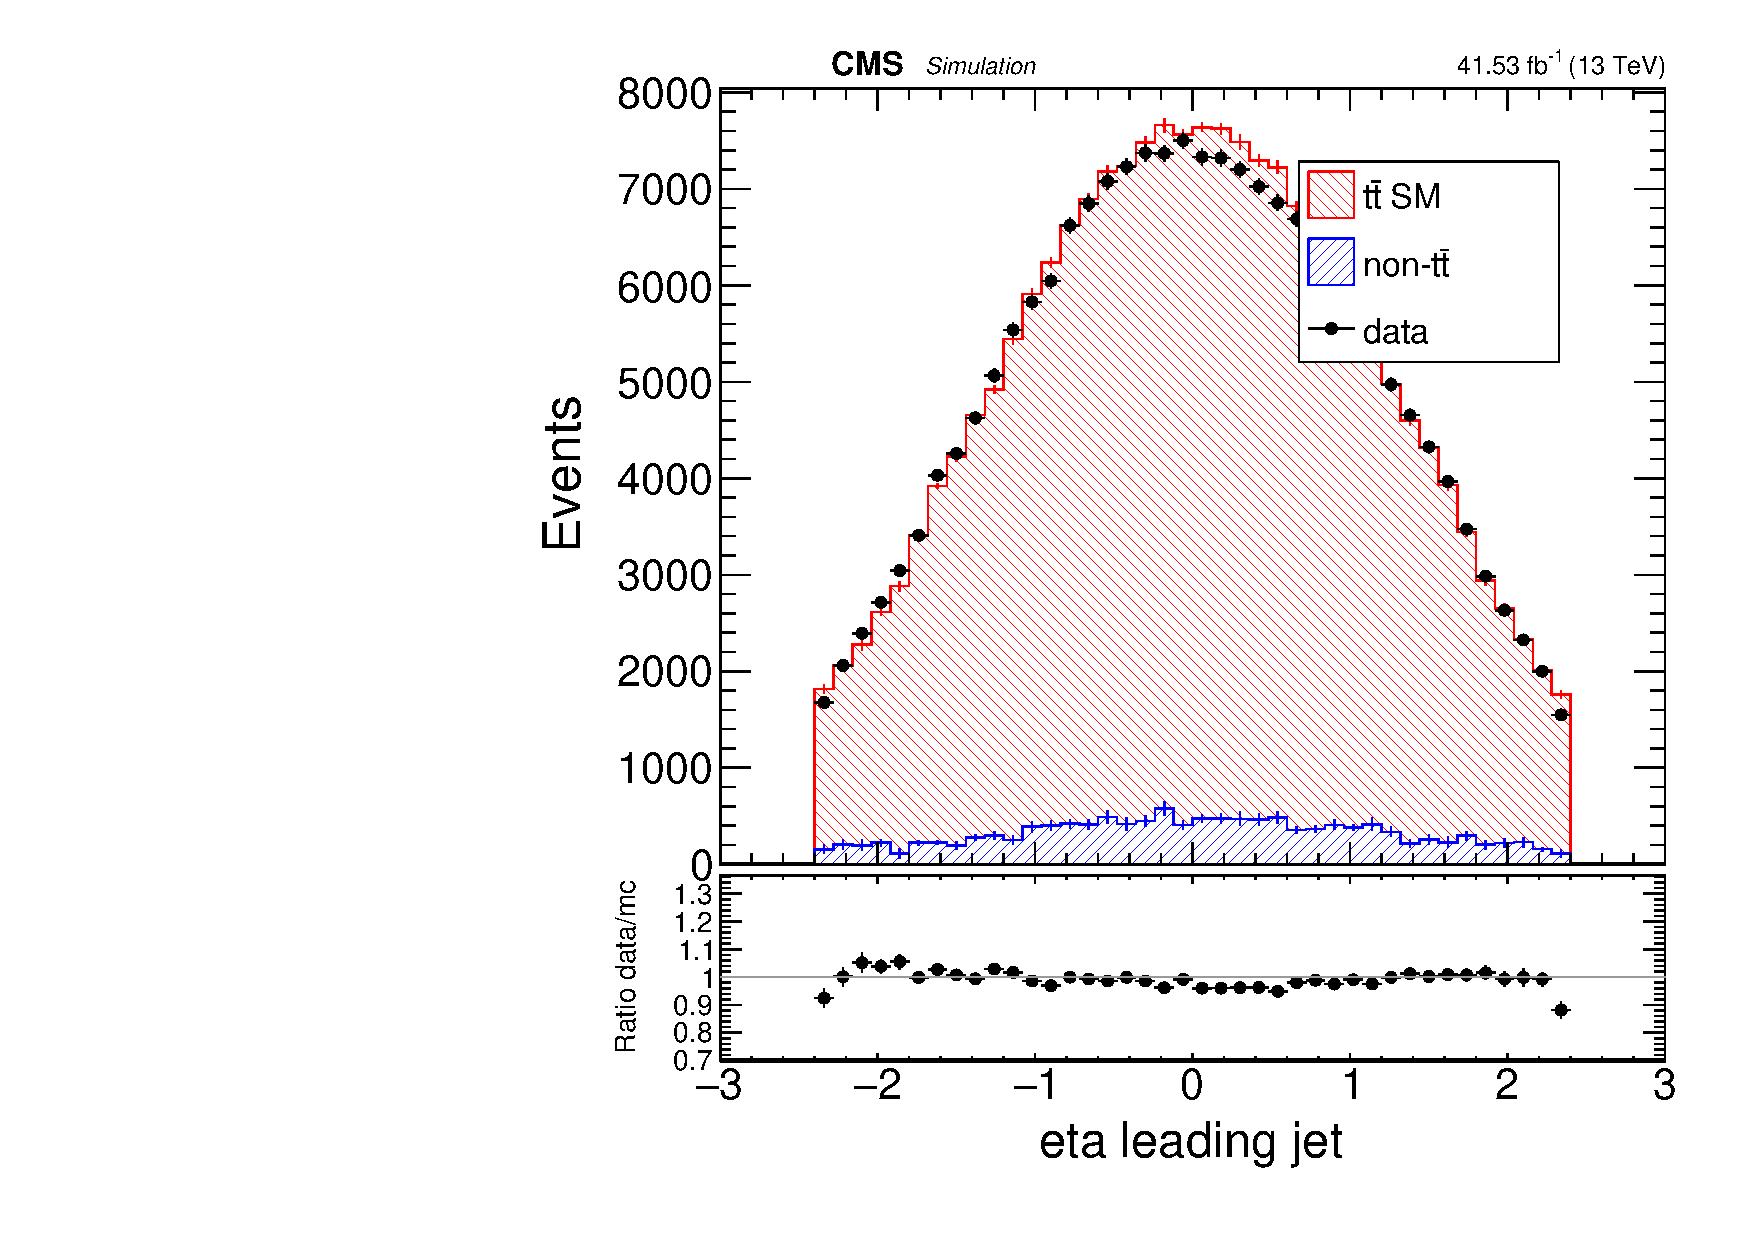
\includegraphics[width=0.8\textwidth, angle=-90]{j1_eta_2017.pdf}
        \caption{2017}
        \label{fig:nb_2017}
    \end{center}
    \end{subfigure}
    \caption{Comparaison données/Monte-Carlo pour le $\eta$ du jet leader pour l'année (\subref{fig:nb_2016}) 2016 et (\subref{fig:nb_2017}) 2017.}
\end{figure}


\section{Incertitudes systématiques}\label{incertsyst}

\begin{figure}[H]
    \begin{subfigure}[b]{0.5\textwidth}
    \begin{center}
        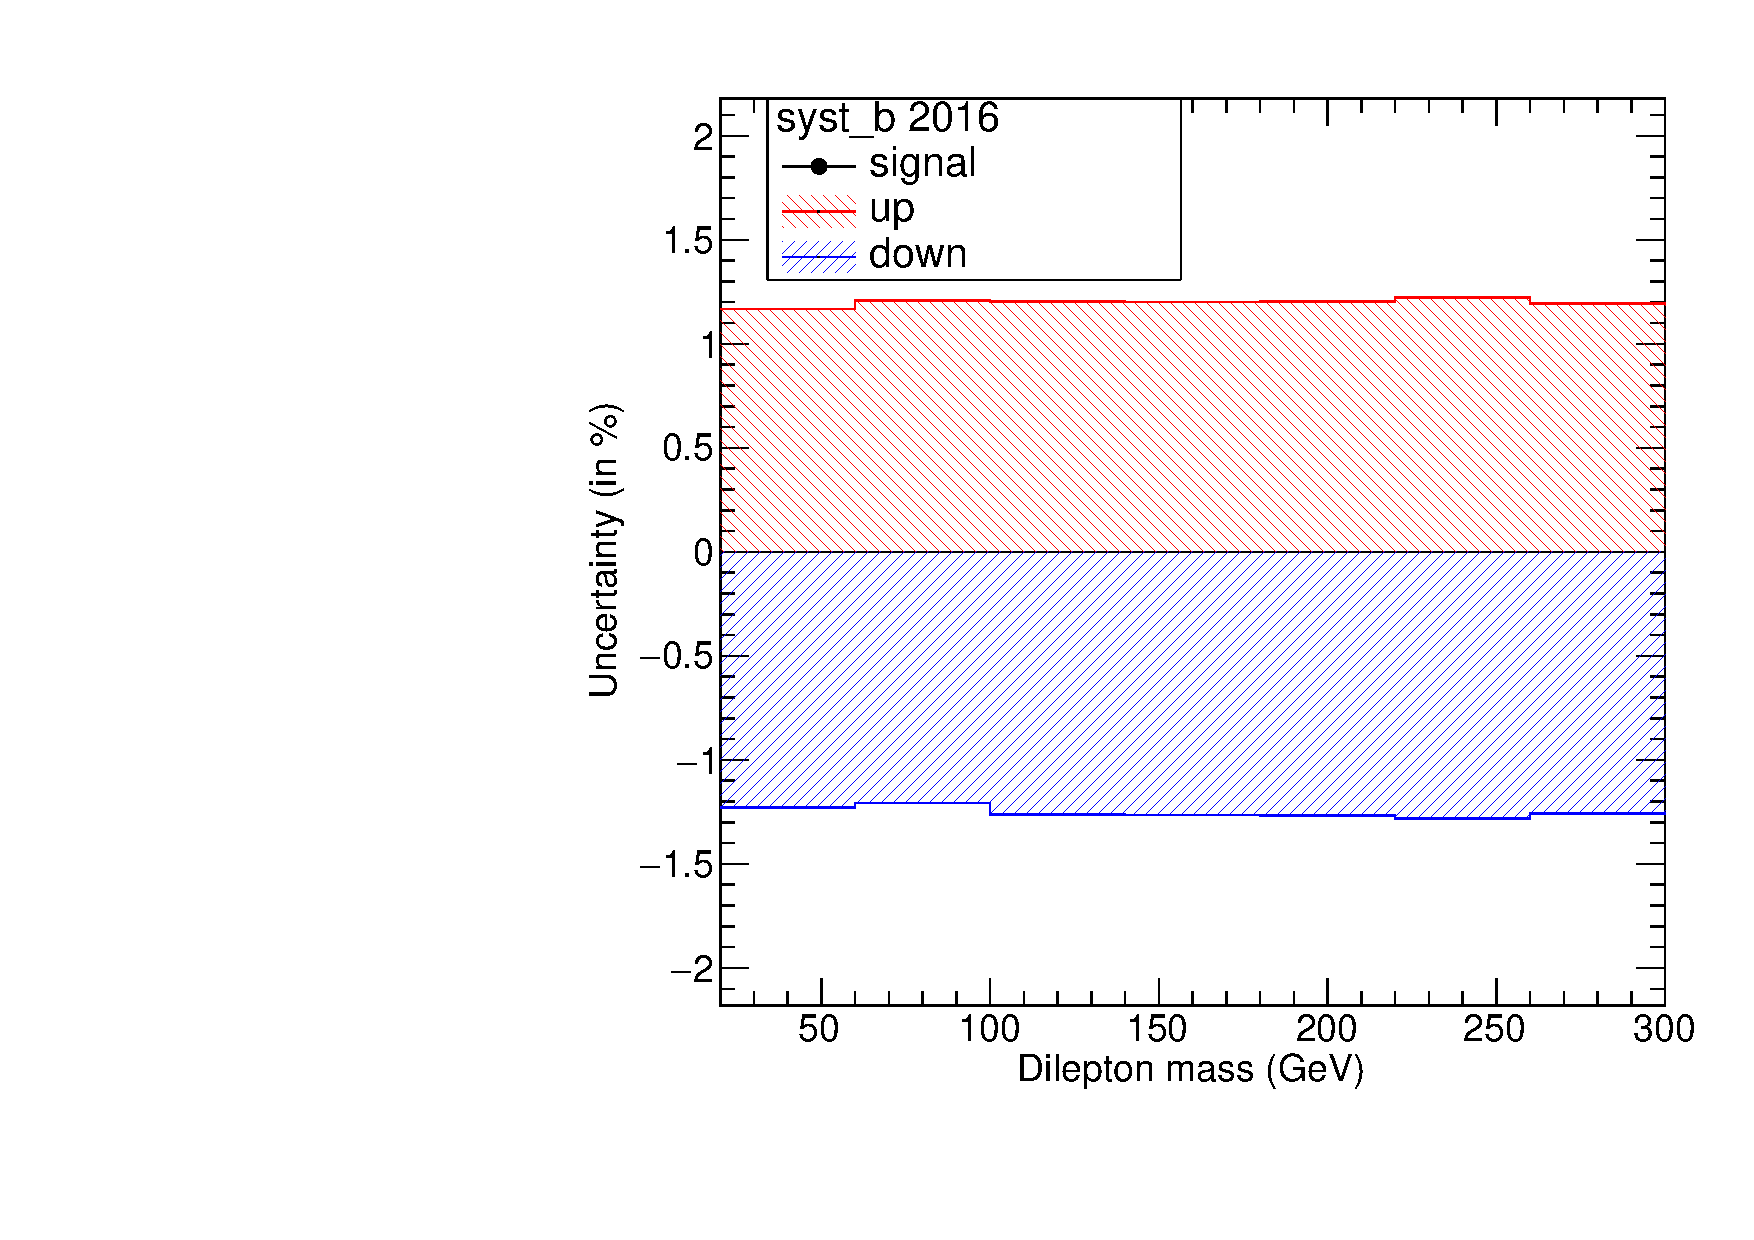
\includegraphics[width=0.8\textwidth, angle=-90]{m_dilep_signal_syst_b_2016.pdf}
        \caption{incertitude sur l'étiquetage des \Pbottom}
        \label{fig:syst_b_2016}
    \end{center}
    \end{subfigure}
        \hspace{0.4cm}
    \begin{subfigure}[b]{0.5\textwidth}
    \begin{center}  
        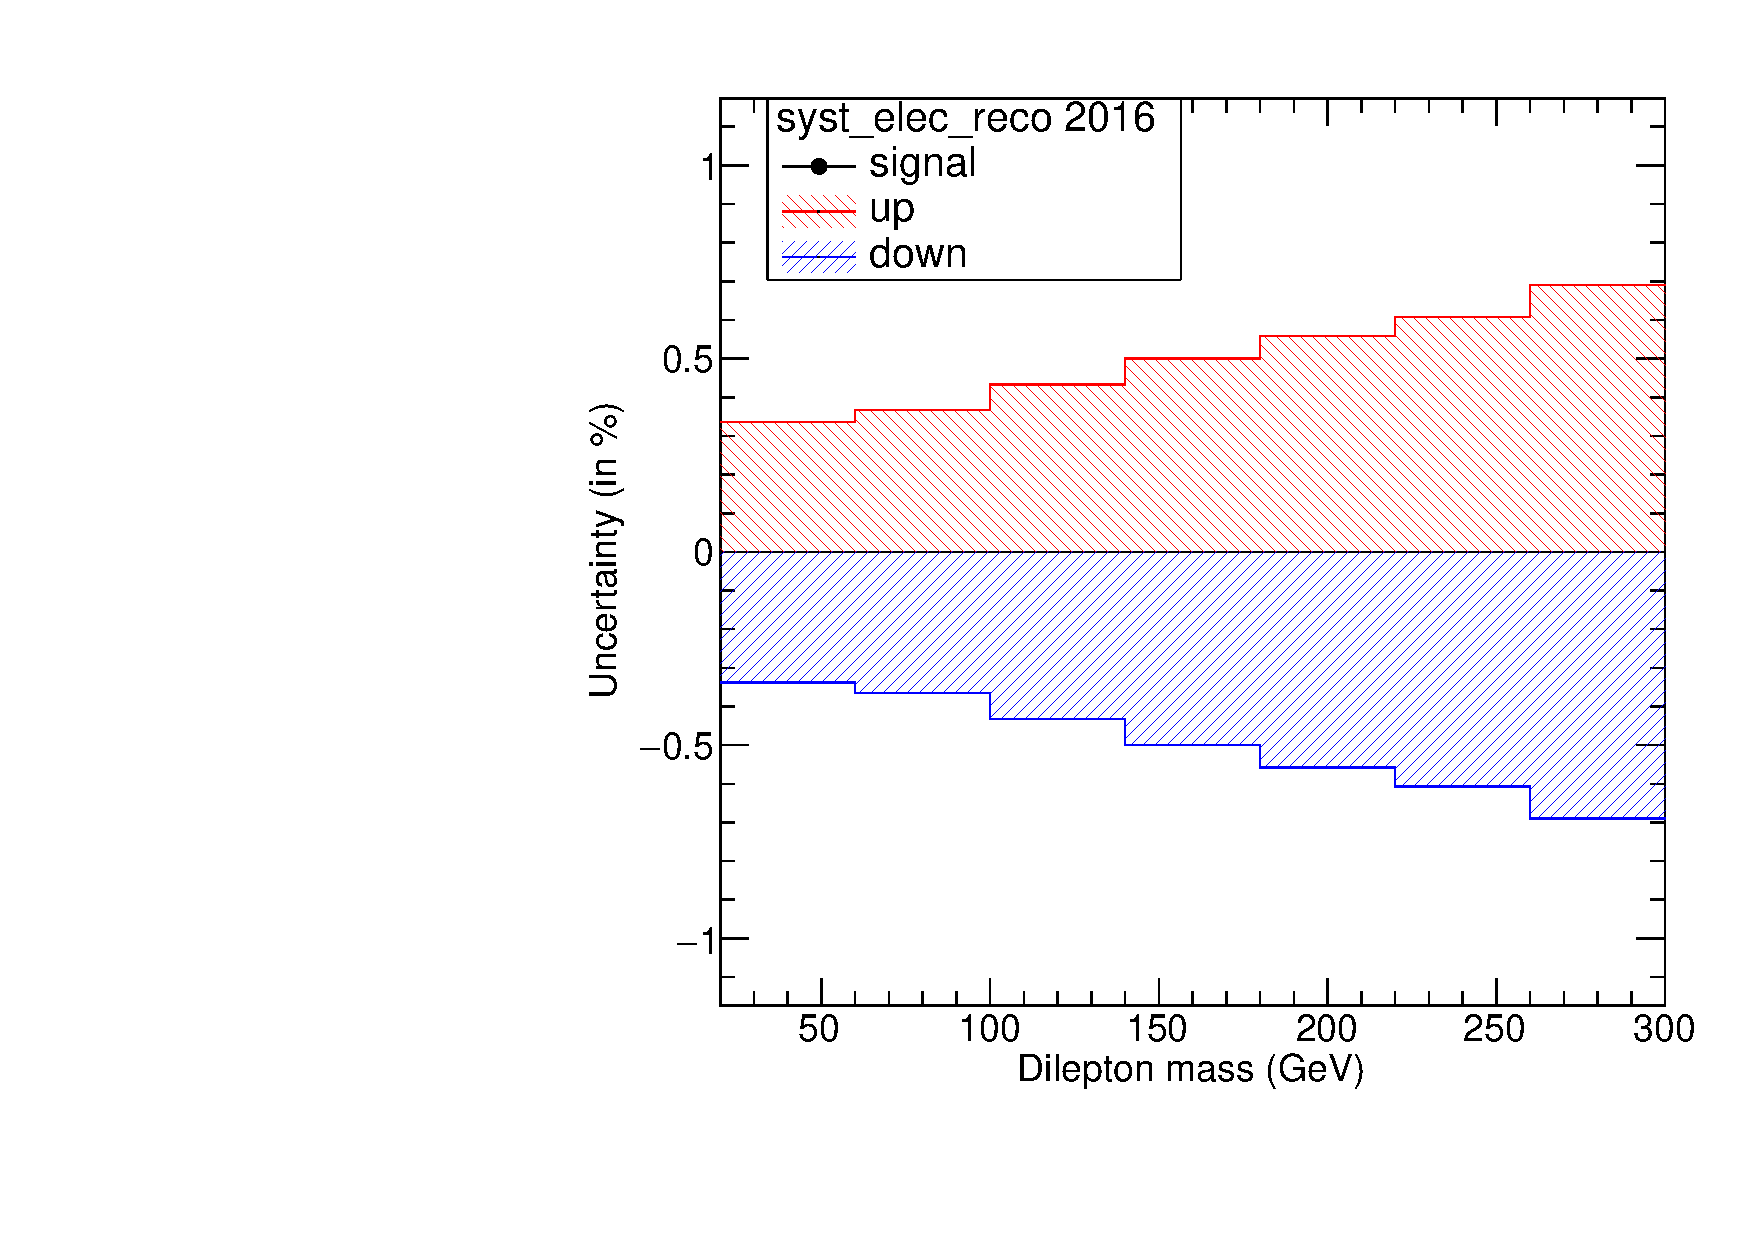
\includegraphics[width=0.8\textwidth, angle=-90]{m_dilep_signal_syst_elec_reco_2016.pdf}
        \caption{incertitude sur la reconstruction des \Pe}
        \label{fig:elec_reco_2016}
    \end{center}
    \end{subfigure}
    \vspace{0.5cm}
    
    \begin{subfigure}[b]{0.5\textwidth}
    \begin{center}
        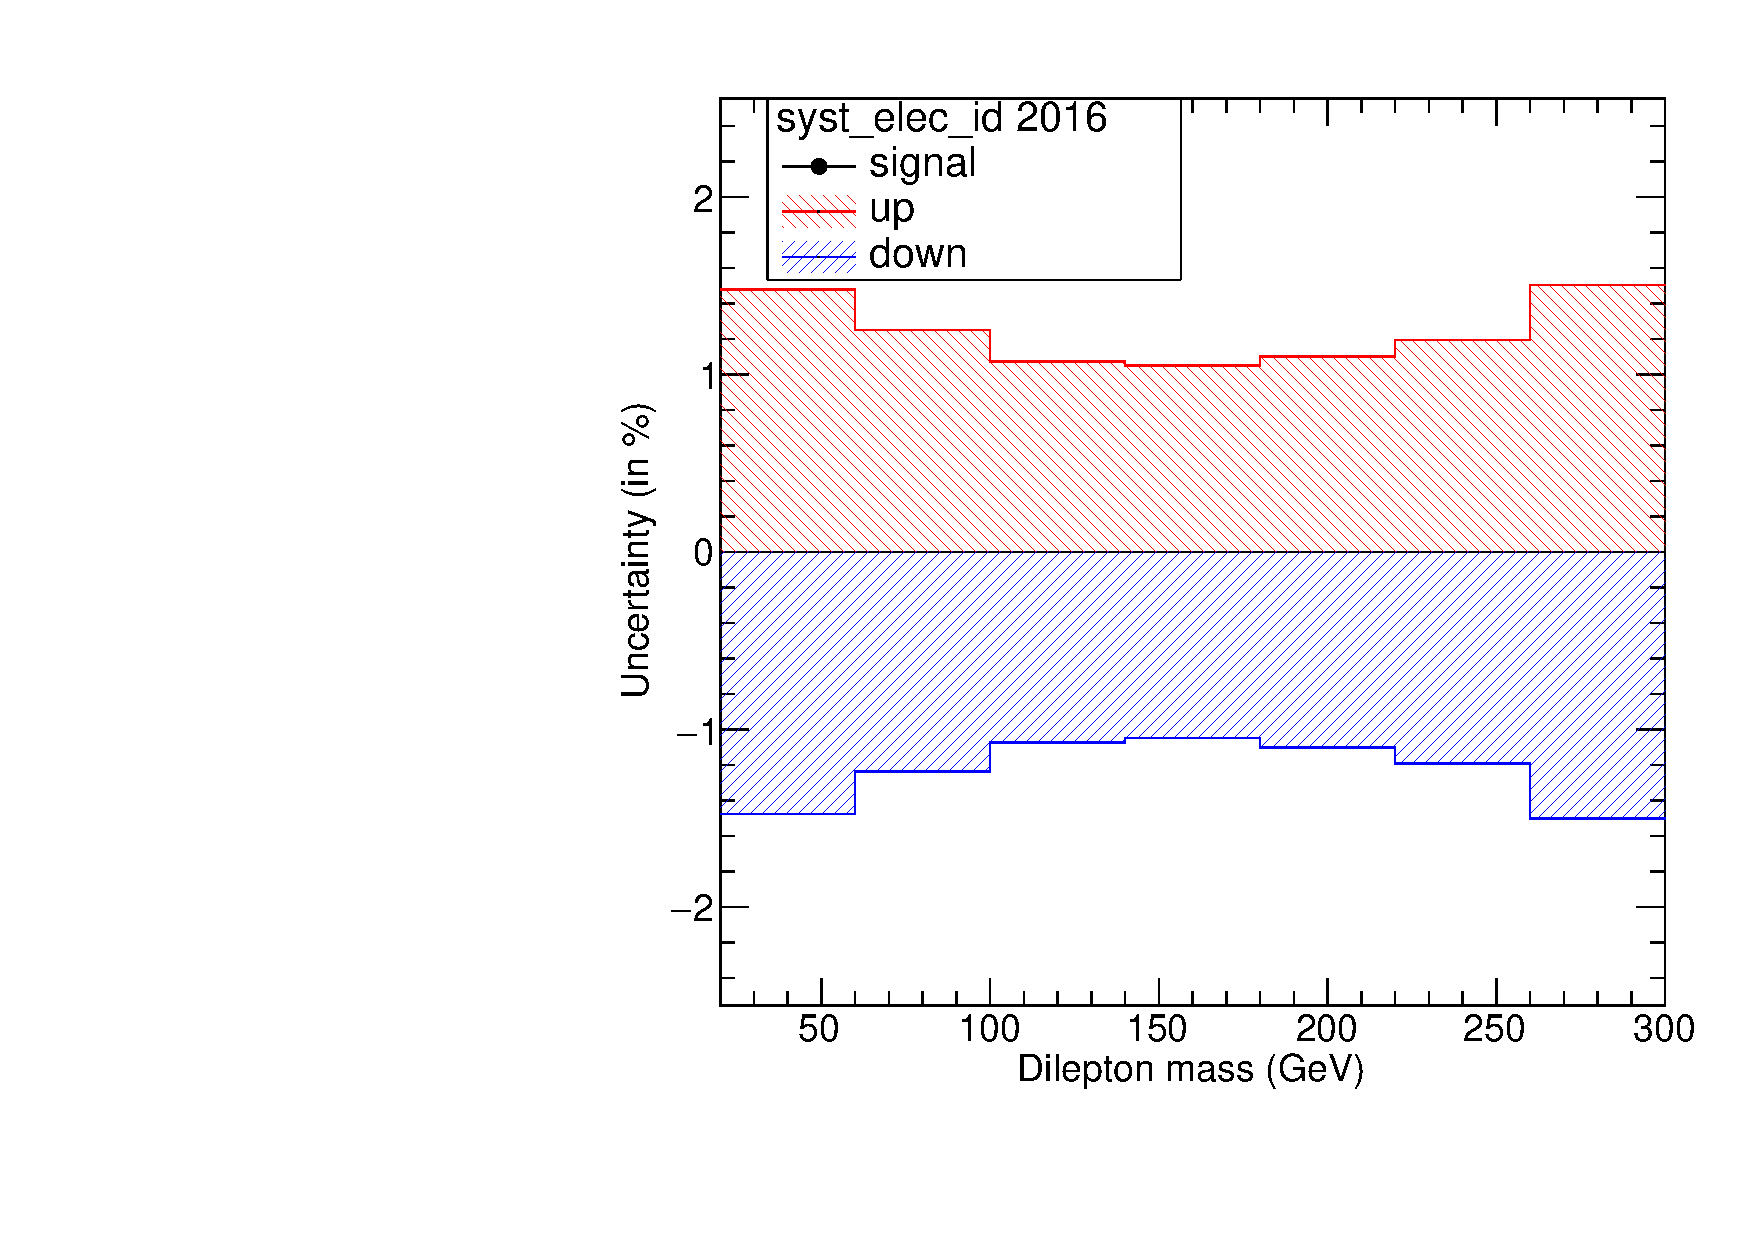
\includegraphics[width=0.8\textwidth, angle=-90]{m_dilep_signal_syst_elec_id_2016.pdf}
        \caption{incertitude sur l'identification des \Pe}
        \label{fig:elec_id_2016}
    \end{center}
    \end{subfigure}
    \hspace{0.4cm}
    \begin{subfigure}[b]{0.5\textwidth}
    \begin{center}
        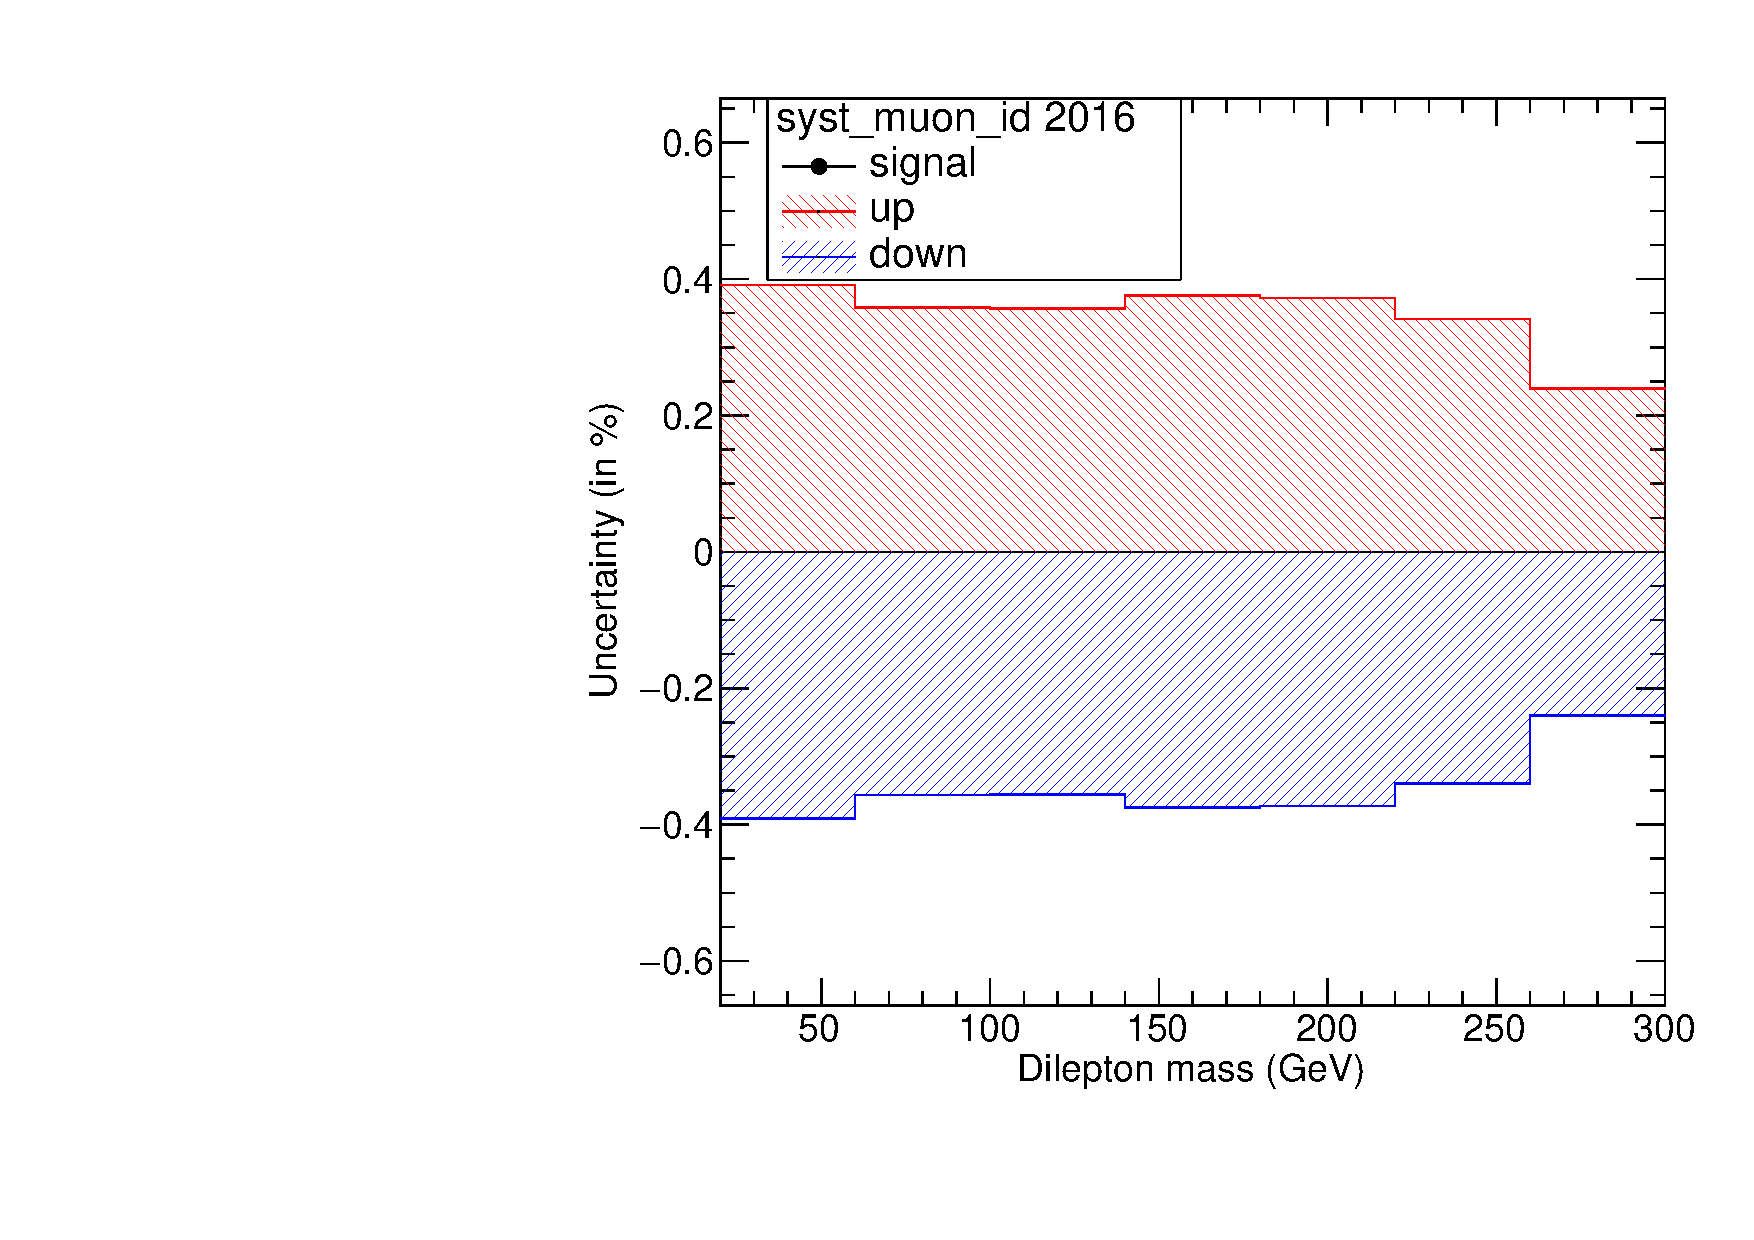
\includegraphics[width=0.8\textwidth, angle=-90]{m_dilep_signal_syst_muon_id_2016.pdf}
        \caption{incertitude sur l'identification des \Pmu}
        \label{fig:muon_id_2016}
    \end{center}
    \end{subfigure}
    \caption{Tracé des incertitudes systématiques pour l'année 2016 avec (\subref{fig:syst_b_2016}) étiquetage des \Pbottom, (\subref{fig:elec_reco_2016}) reconstruction des électrons, (\subref{fig:elec_id_2016}) identification des électrons et (\subref{fig:muon_id_2016}) identification des muons sur la masse dilepton de l'échantillon Monte-Carlo \ttbar. Chaque histogramme présente des incertitudes relatives.}
\end{figure}


\begin{figure}[H]
    \begin{subfigure}[b]{0.5\textwidth}
    \begin{center}
        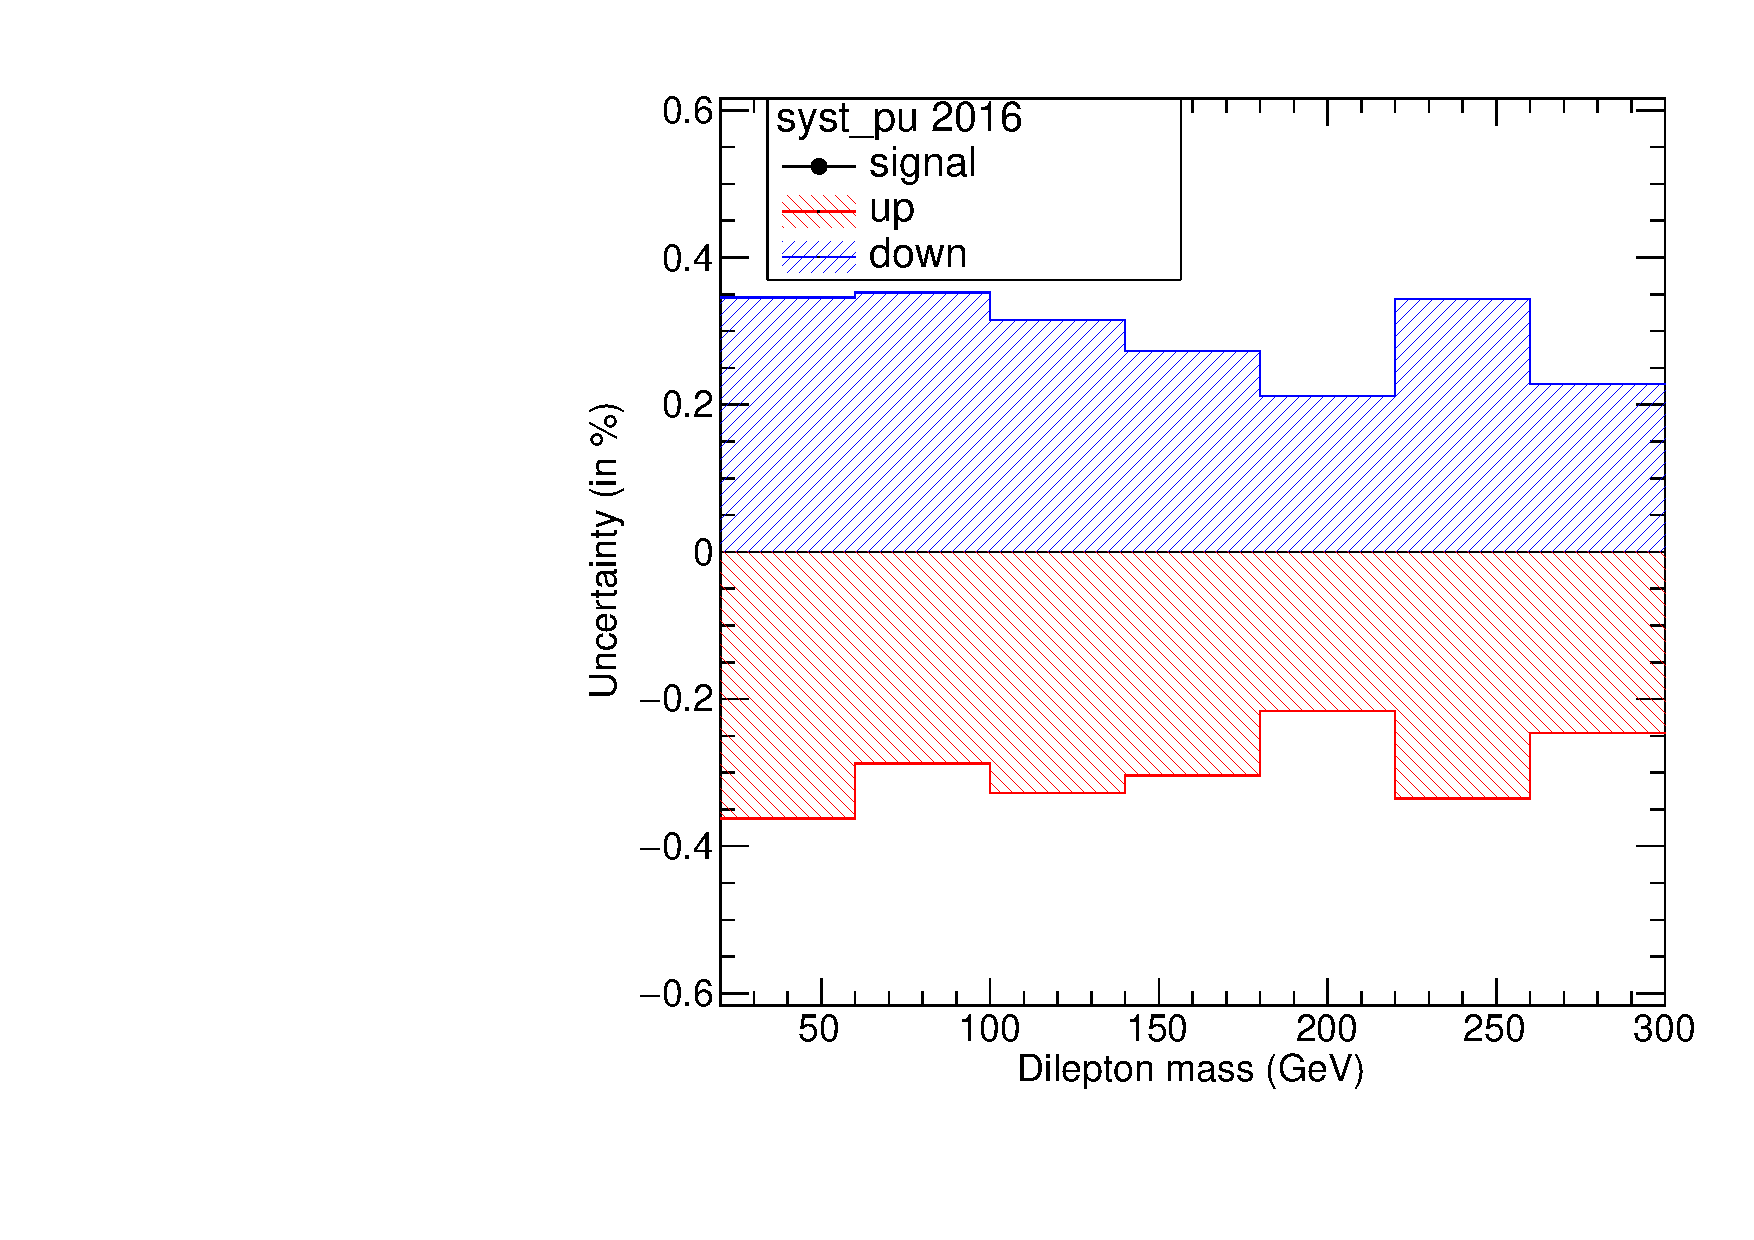
\includegraphics[width=0.8\textwidth, angle=-90]{m_dilep_signal_syst_pu_2016.pdf}
        \caption{2016}
        \label{fig:pu2016}
    \end{center}
    \end{subfigure}
    \begin{subfigure}[b]{0.5\textwidth}
    \begin{center}
        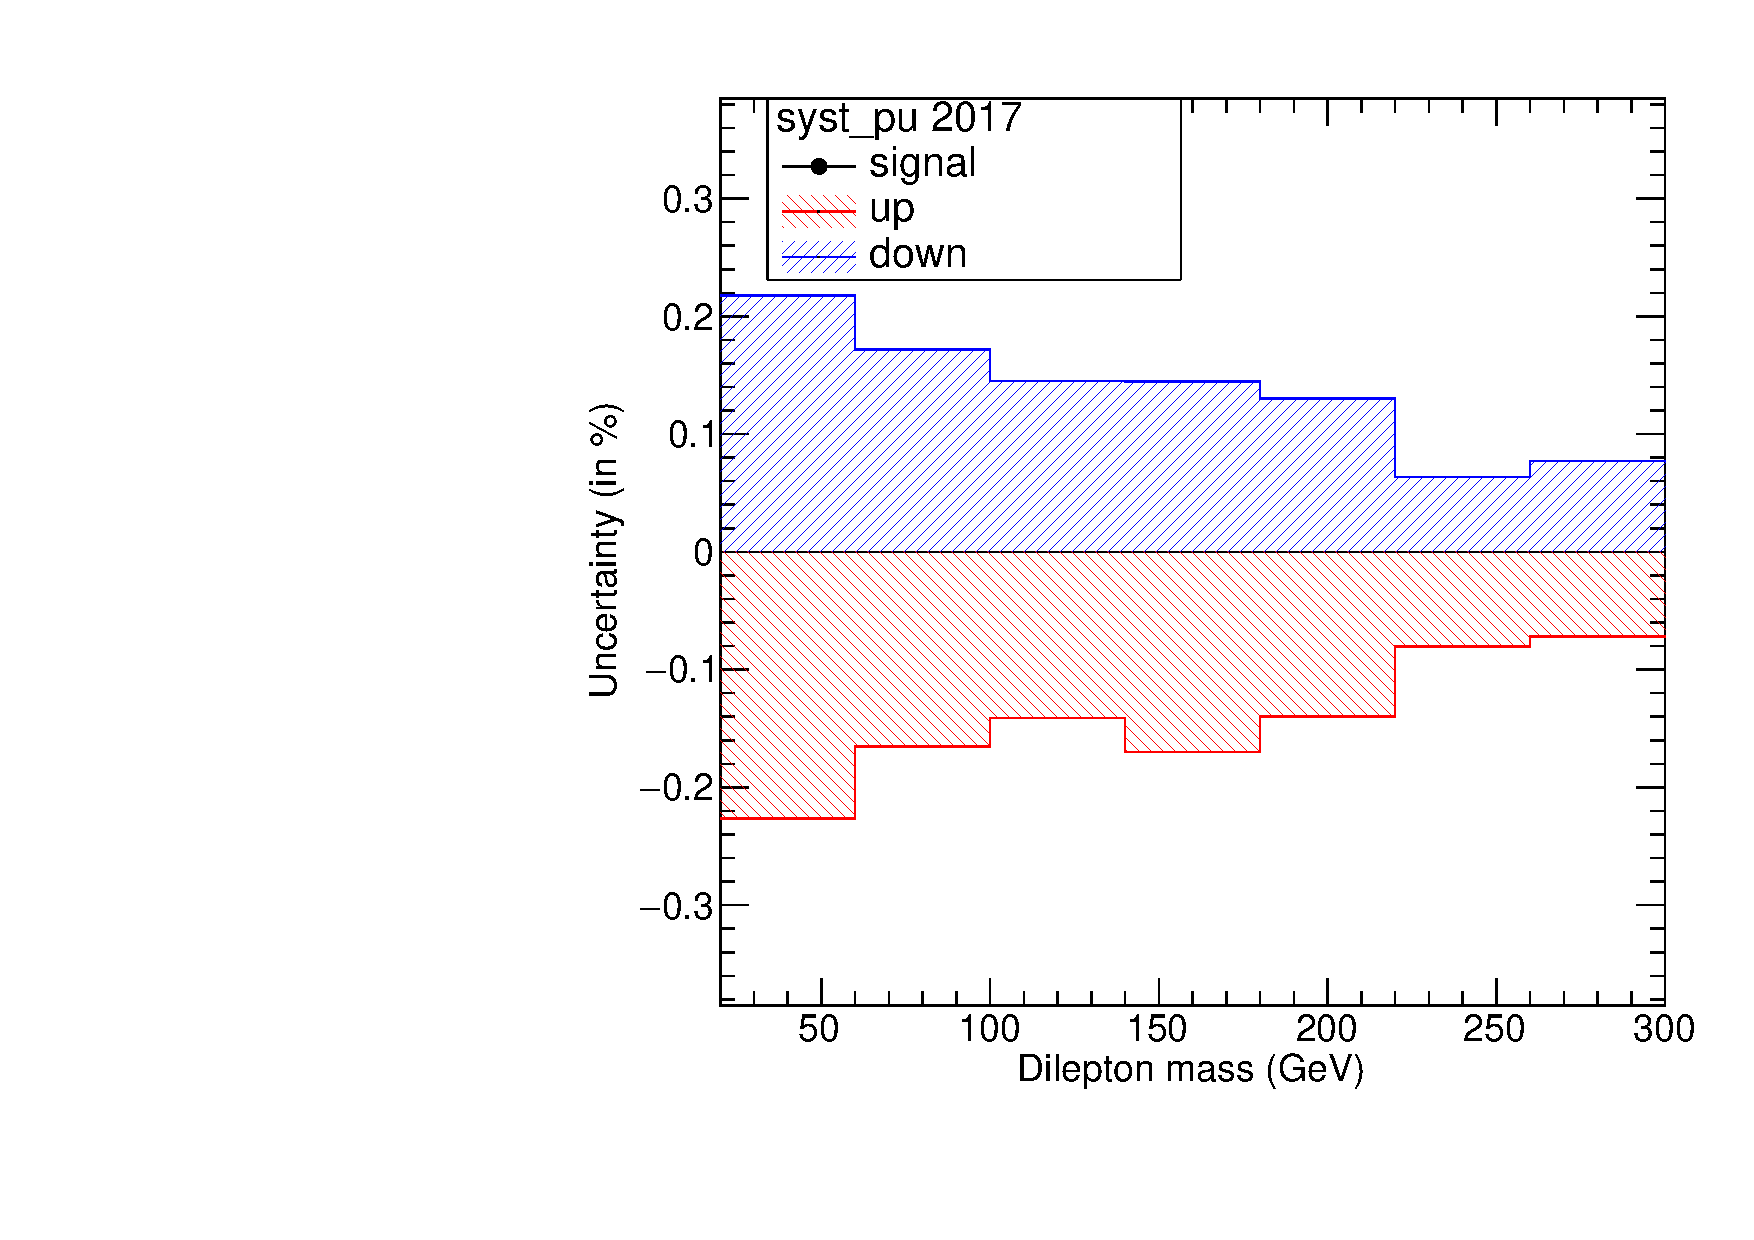
\includegraphics[width=0.8\textwidth, angle=-90]{m_dilep_signal_syst_pu_2017.pdf}
        \caption{2017}
        \label{fig:pu2017}
    \end{center}
    \end{subfigure}
    \caption{Tracé des incertitudes systématiques du \emph{pile-up} sur la masse dilepton de l'échantillon Monte-Carlo \ttbar. Chaque histogramme présente des incertitudes relatives pour l'année (\subref{fig:pu2016}) 2016 et (\subref{fig:pu2017}) 2017.}
\end{figure}

\end{fmffile}
